%yright 2007, 2008, 2009 Elsevier Ltd
%% 
%% This file is part of the 'Elsarticle Bundle'.
%% ---------------------------------------------
%% 
%% It may be distributed under the conditions of the LaTeX Project Public
%% License, either version 1.2 of this license or (at your option) any
%% later version.  The latest version of this license is in
%%    http://www.latex-project.org/lppl.txt
%% and version 1.2 or later is part of all distributions of LaTeX
%% version 1999/12/01 or later.
%% 
%% The list of all files belonging to the 'Elsarticle Bundle' is
%% given in the file `manifest.txt'.
%% 

%% Template article for Elsevier's document class `elsarticle'
%% with numbered style bibliographic references
%% SP 2008/03/01

% \documentclass[preprint,11pt]{elsarticle}
\documentclass[final,1p,11pt]{elsarticle}

%\documentclass[final,1p,times]{elsarticle}


%% Use the option review to obtain double line spacing
%%\documentclass[authoryear,preprint,review,12pt]{elsarticle}

%% Use the options 1p,twocolumn; 3p; 3p,twocolumn; 5p; or 5p,twocolumn
%% for a journal layout:
%% \documentclass[final,1p,times]{elsarticle}
%% \documentclass[final,1p,times,twocolumn]{elsarticle}
%% \documentclass[final,3p,times]{elsarticle}
%% \documentclass[final,3p,times,twocolumn]{elsarticle}
%% \documentclass[final,5p,times]{elsarticle}
%% \documentclass[final,5p,times,twocolumn]{elsarticle}

%%% For including figures, graphicx.sty has been loaded in
%% elsarticle.cls. If you prefer to use the old commands
%% please give \usepackage{epsfig}


\usepackage{epsfig}
%\usepackage{cite}
%\usepackage{mcite}
\usepackage{array,tabularx,epsfig,mathrsfs,graphicx,rotating}
\usepackage{ifthen}
\usepackage{amsfonts}
\usepackage{ragged2e}
\PassOptionsToPackage{hyphens}{url}
\usepackage[hyphens]{url}
\usepackage{hyperref}
\usepackage{listings}
\usepackage{subfigure}
\usepackage{epstopdf}
% Custom colors
\usepackage{color}
\usepackage{float}

% to cross text
\usepackage[normalem]{ulem} % either use this (simple) or
\usepackage{soul} % use this (many fancier options)


\hypersetup{
  colorlinks=true,
  linkcolor=blue,
  citecolor=blue,
  urlcolor=blue
}




\graphicspath{{figs/}}


\pdfinfo{
   /Author (Chekanov/Demarteau)
   /Title  (Conceptual Design Studies for a CEPC Detector)
   /CreationDate (D:20160102195600)
   /Subject (PDFLaTeX)
   /Keywords (PDF;LaTeX)
}


\textheight=22cm
\textwidth=14.5cm

\newcommand{\beq}{\begin{equation}}
\newcommand{\eeq}{\end{equation}}
\newcommand{\la}{\langle}
\newcommand{\promc}{{\sc ProMC}}
\newcommand{\ra}{\rangle}
\newcommand{\eps}{\epsilon}
\newcommand{\ud}{\mathrm{d}}
\newcommand{\Ec}{\mathcal{E}}
\newcommand{\Fc}{\mathcal{F}}
\newcommand{\Za}{\mathrm{Z_1}}
\newcommand{\Zb}{\mathrm{Z_2}}
\newcommand{\Zn}{\mathrm{Z_n}}
\newcommand{\F}{\mathrm{F}}

\chardef\til=126
\newcommand{\mev}{{\,\mathrm{MeV}}}
\newcommand{\gev}{{\,\mathrm{GeV}}}
\newcommand{\tev}{{\,\mathrm{TeV}}}
\newcommand{\GEANTfour} {\textsc{geant4}}
\journal{XXX-XXX}



\begin{document}

\section{Studies of signal and background separation using Mass soft drop at $\beta=0$ using fix central and change width method}

\label{sec:Mann Whitney U test}

%50bins
\begin{figure}
\begin{center}
   \subfigure[5TeV at 20$\times$20(cm$\times$cm) in cluster] {
   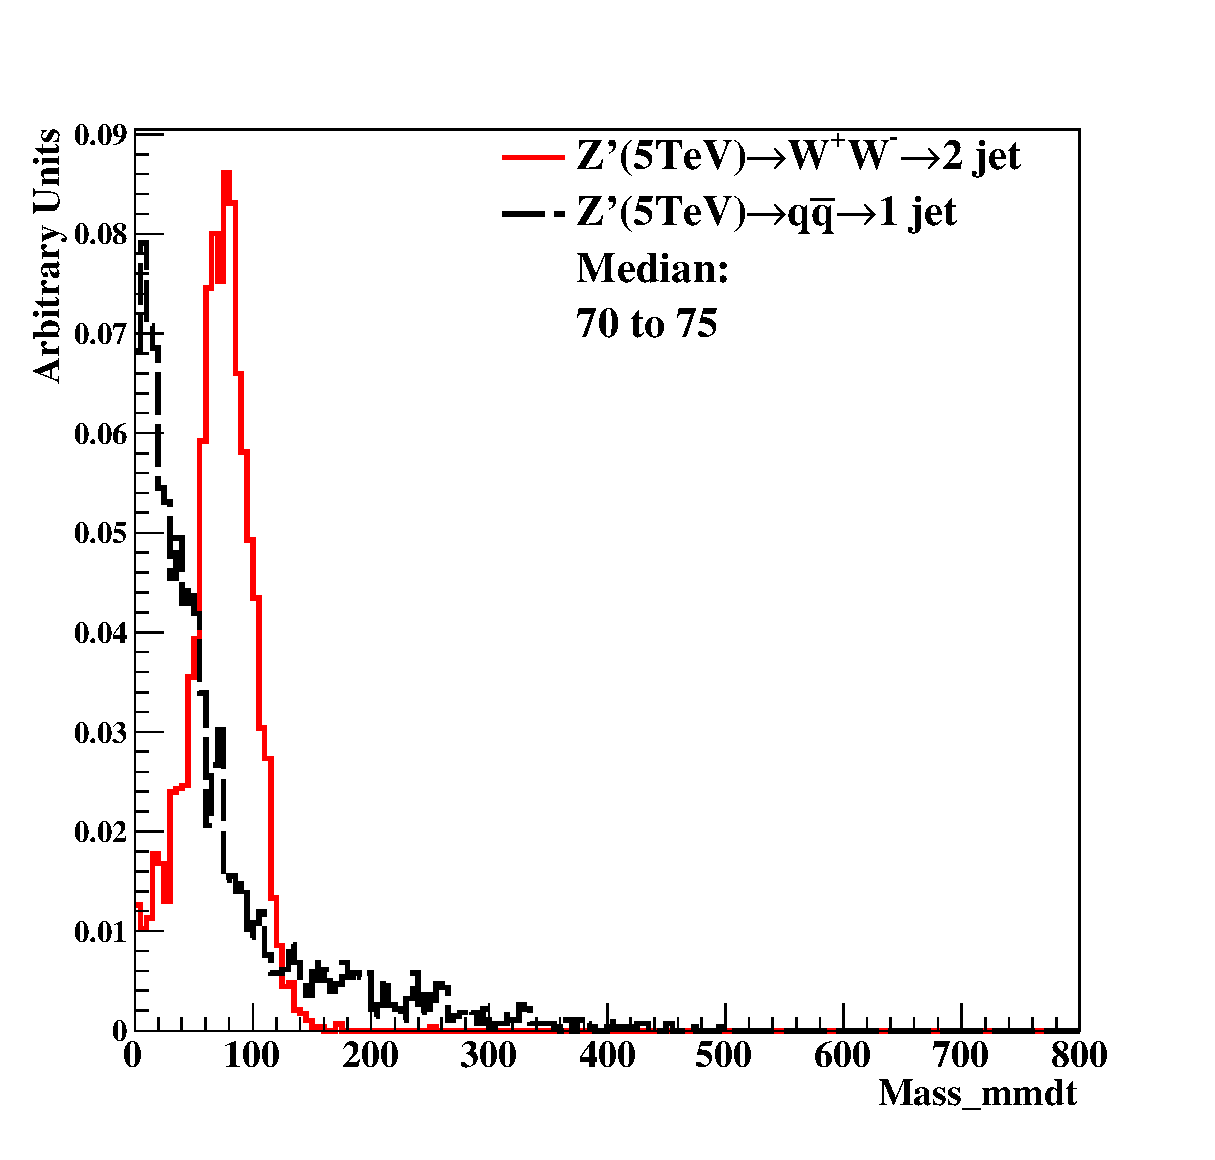
\includegraphics[width=0.43\textwidth]{figs/Dis_cluster_010_mass_mmdt_5tev_04.eps}\hfill
   }
   \subfigure[5TeV at 5$\times$5(cm$\times$cm) in cluster] {
   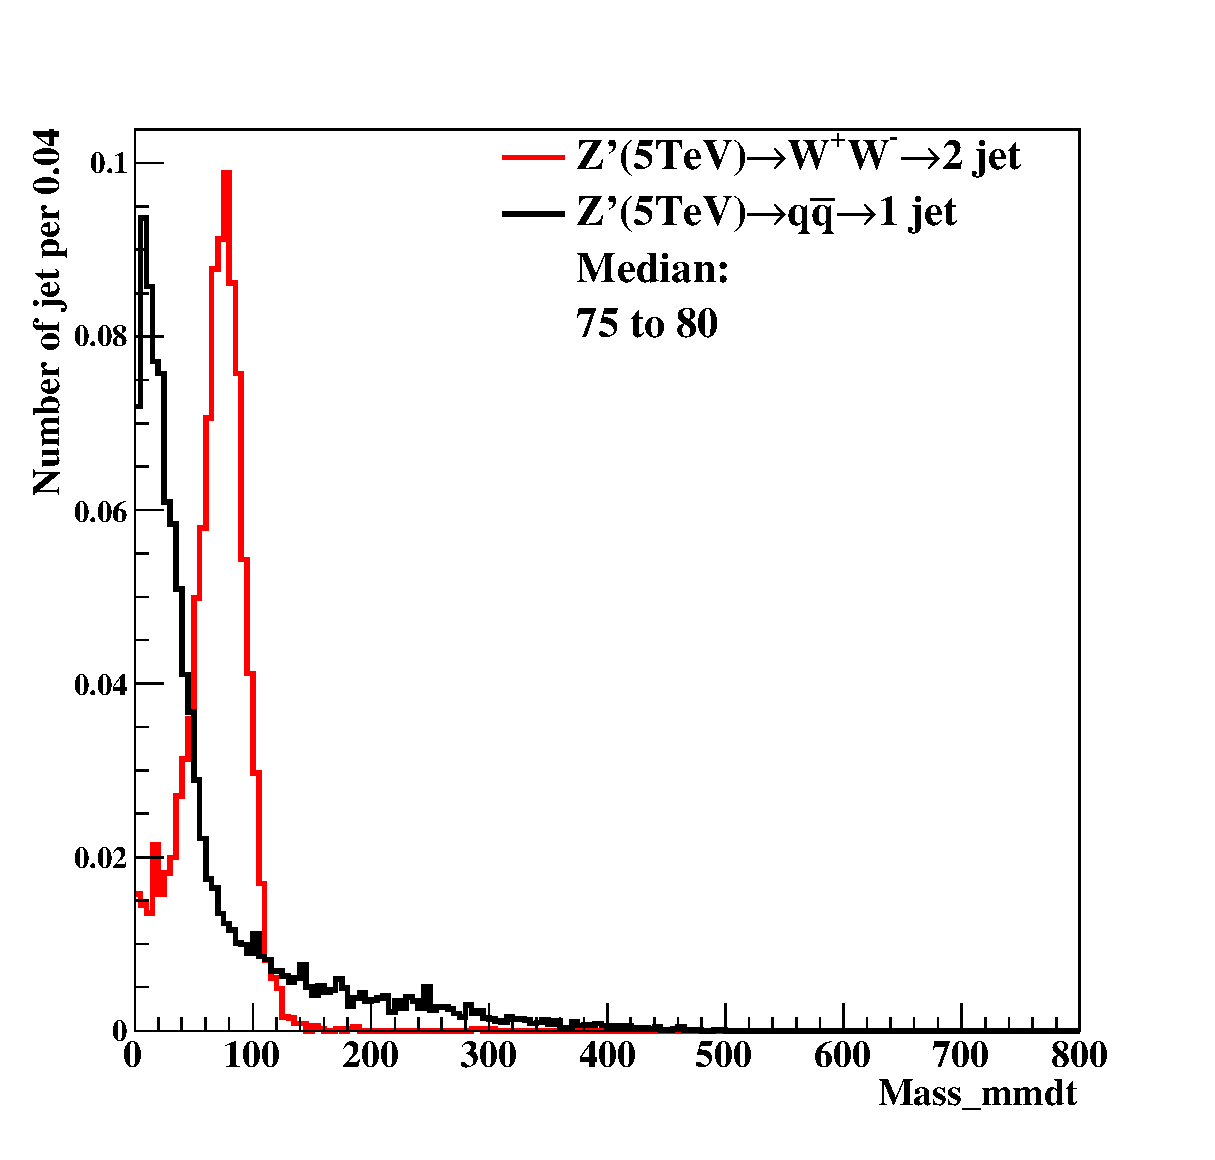
\includegraphics[width=0.43\textwidth]{figs/Dis_cluster_009_mass_mmdt_5tev_04.eps}
   }
   \subfigure[5TeV at 1$\times$1(cm$\times$cm) in cluster] {
   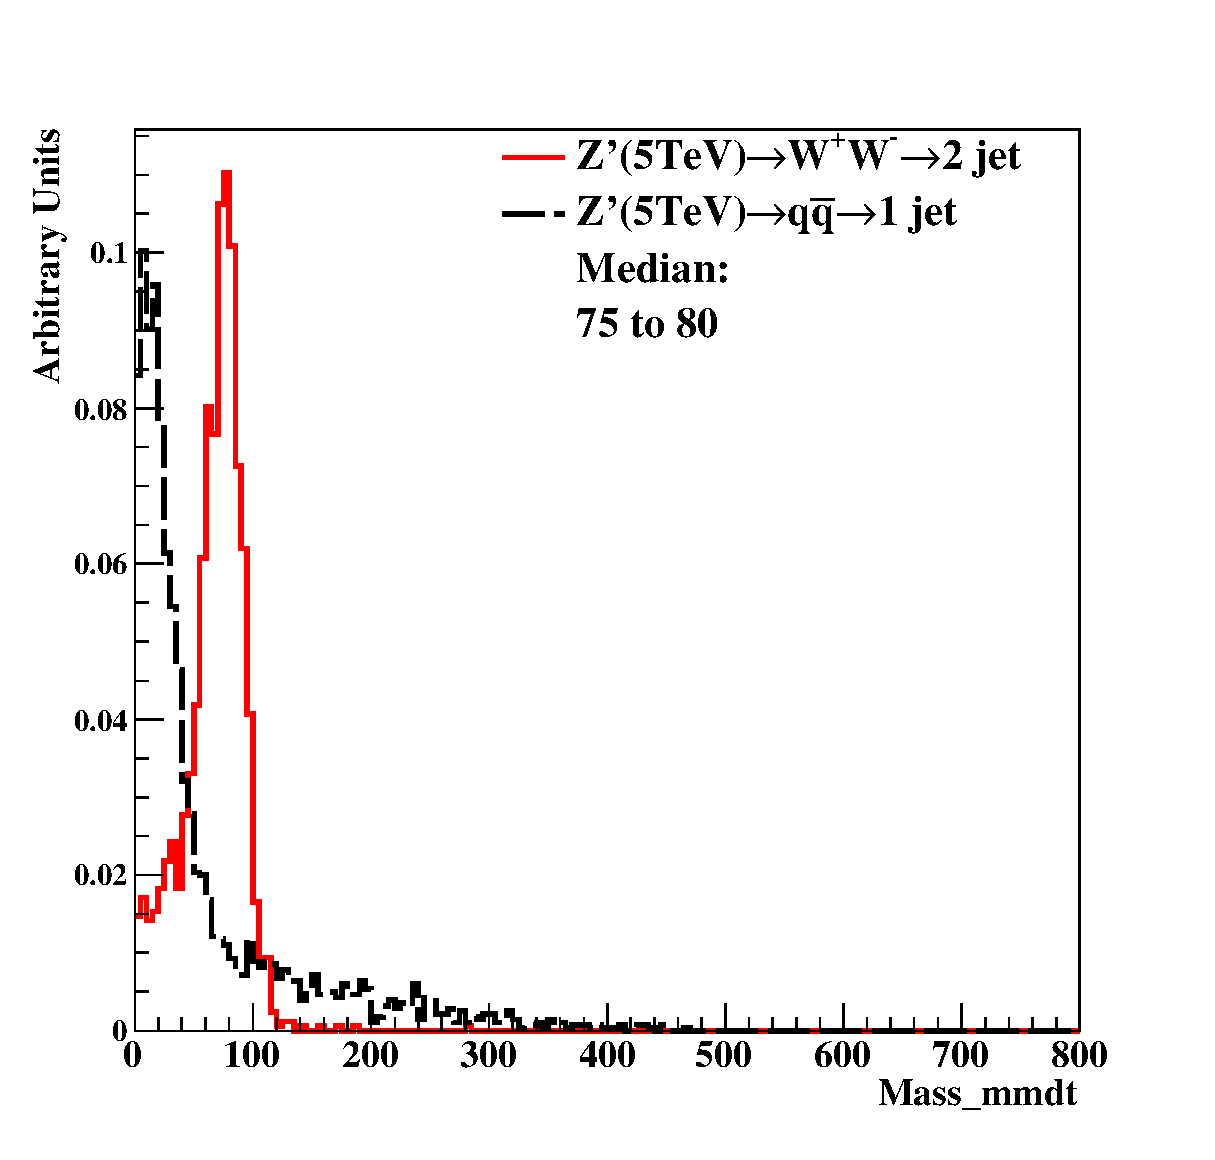
\includegraphics[width=0.43\textwidth]{figs/Dis_cluster_012_mass_mmdt_5tev_04.eps}
   }

\end{center}
\caption{Distributions of mass soft drop at $\beta$=0, signal=ww, in 5TeV energy of collision  in different detector sizes. Cell Size in 20$\times$20, 5$\times$5, and 1$\times$1(cm$\times$cm) are shown here.}
\label{fig:cluster_tau21_tau32}
\end{figure}

\begin{figure}
\begin{center}
   \subfigure[Central at 60TeV change width in cluster ] {
   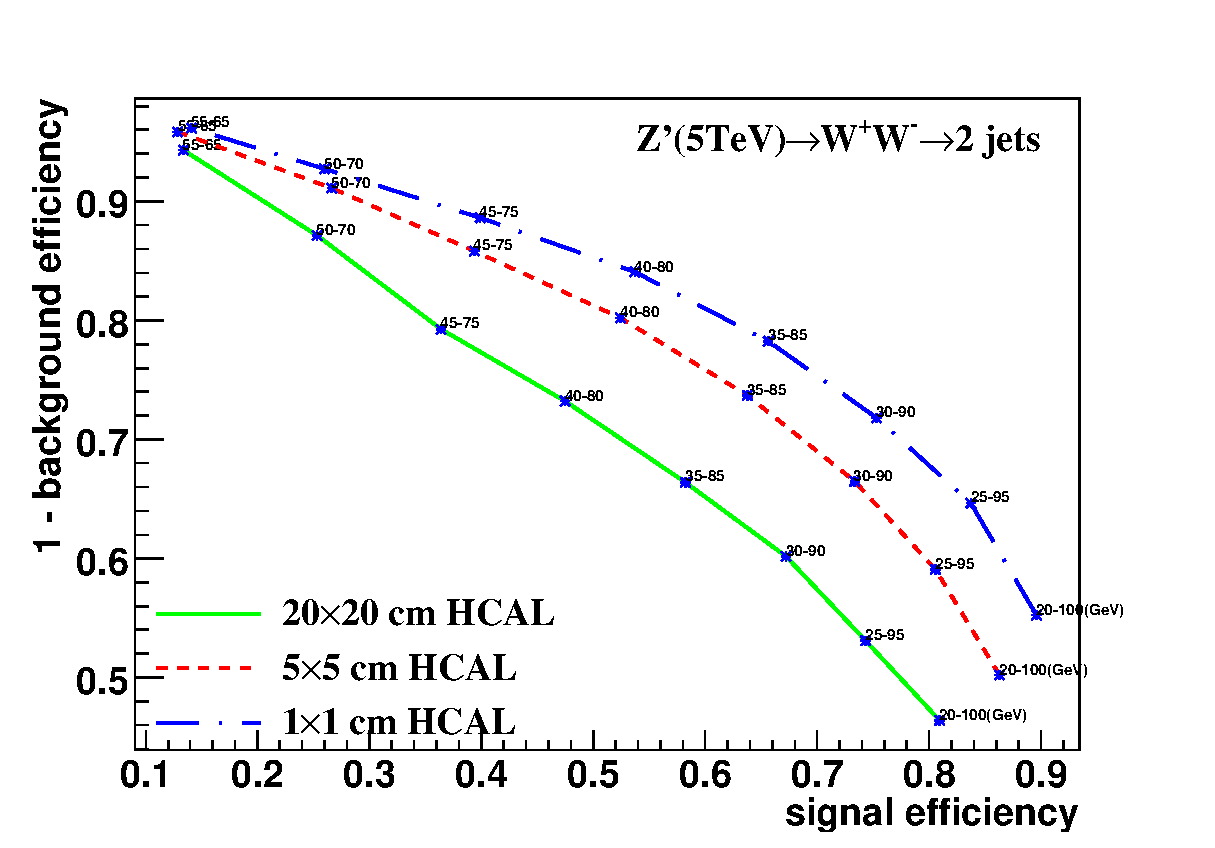
\includegraphics[width=0.43\textwidth]{figs/A_Cluster_mass_mmdt_5tev_eff_1_central_fix_at_60GeV_ww_qq.eps}\hfill
   }
   \subfigure[Central at 65TeV change width in cluster] {
   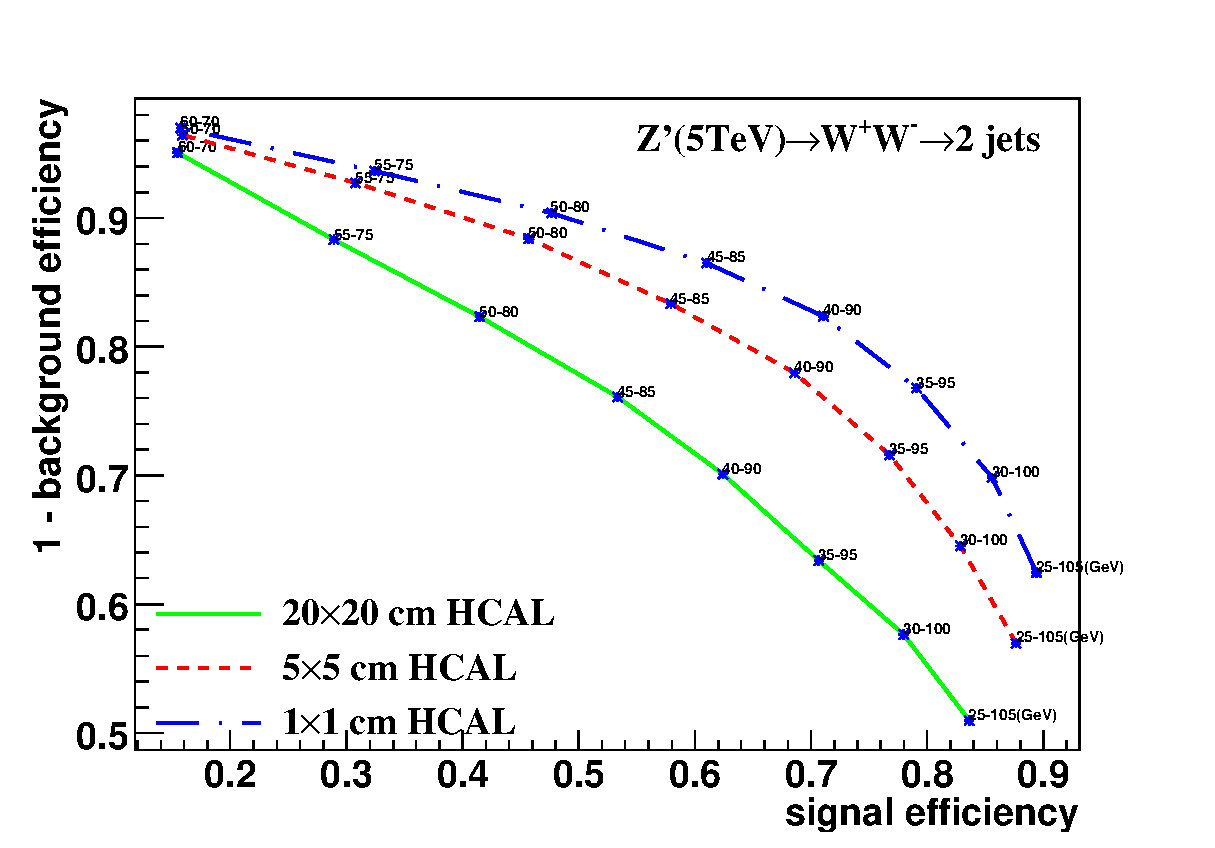
\includegraphics[width=0.43\textwidth]{figs/A_Cluster_mass_mmdt_5tev_eff_1_central_fix_at_65GeV_ww_qq.eps}
   }
   \subfigure[Central at 70TeV change width in cluster] {
   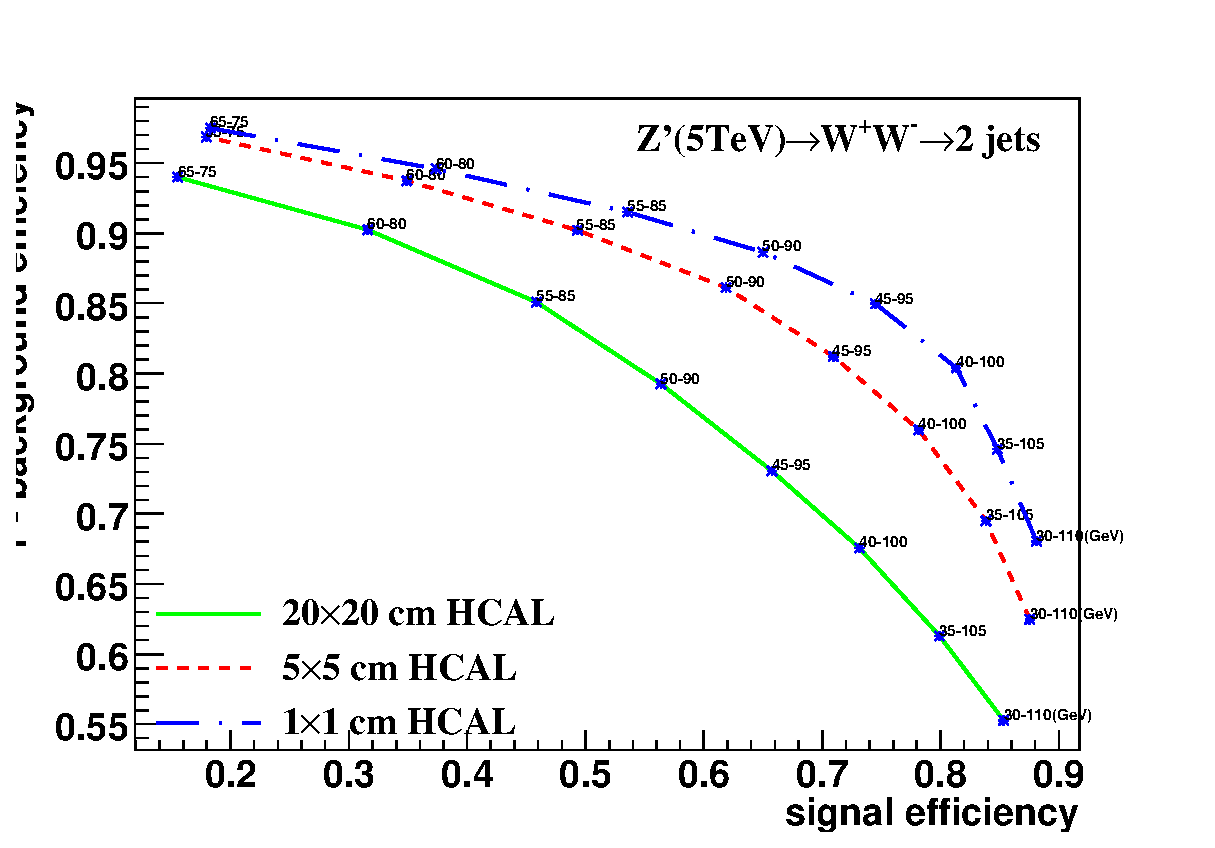
\includegraphics[width=0.43\textwidth]{figs/A_Cluster_mass_mmdt_5tev_eff_1_central_fix_at_70GeV_ww_qq.eps}
   }
   \subfigure[Central at 75TeV change width in cluster] {
   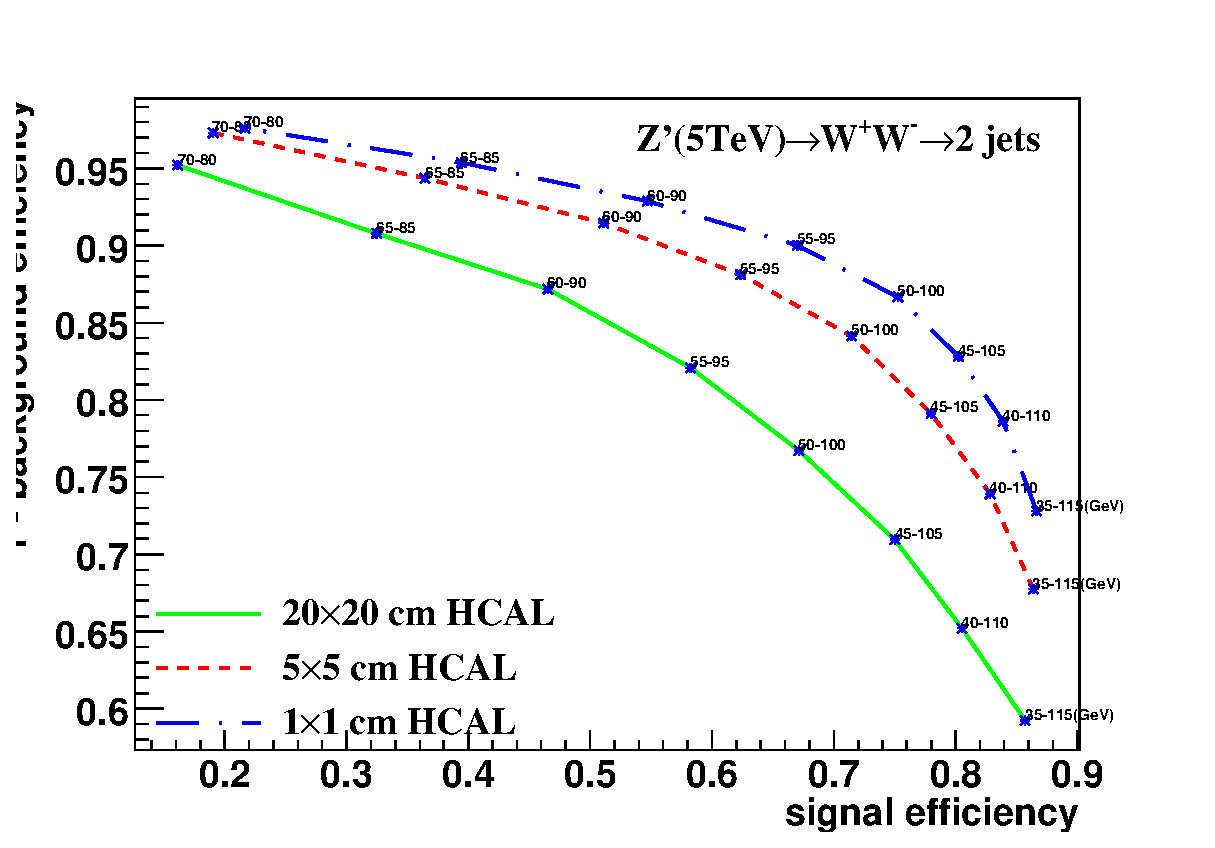
\includegraphics[width=0.43\textwidth]{figs/A_Cluster_mass_mmdt_5tev_eff_1_central_fix_at_75GeV_ww_qq.eps}
   }
   \subfigure[Central at 80TeV change width in cluster] {
   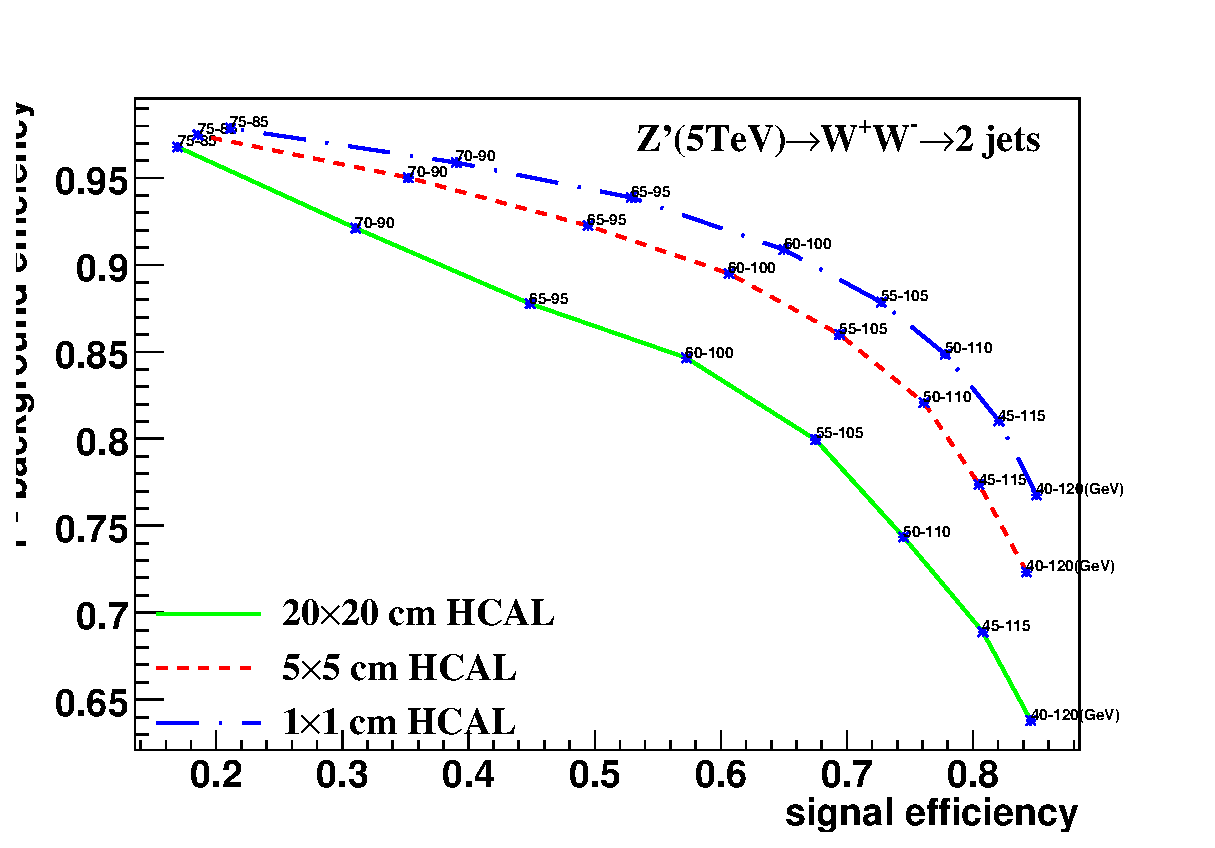
\includegraphics[width=0.43\textwidth]{figs/A_Cluster_mass_mmdt_5tev_eff_1_central_fix_at_80GeV_ww_qq.eps}
   }
   \subfigure[Central at 85TeV change width in cluster] {
   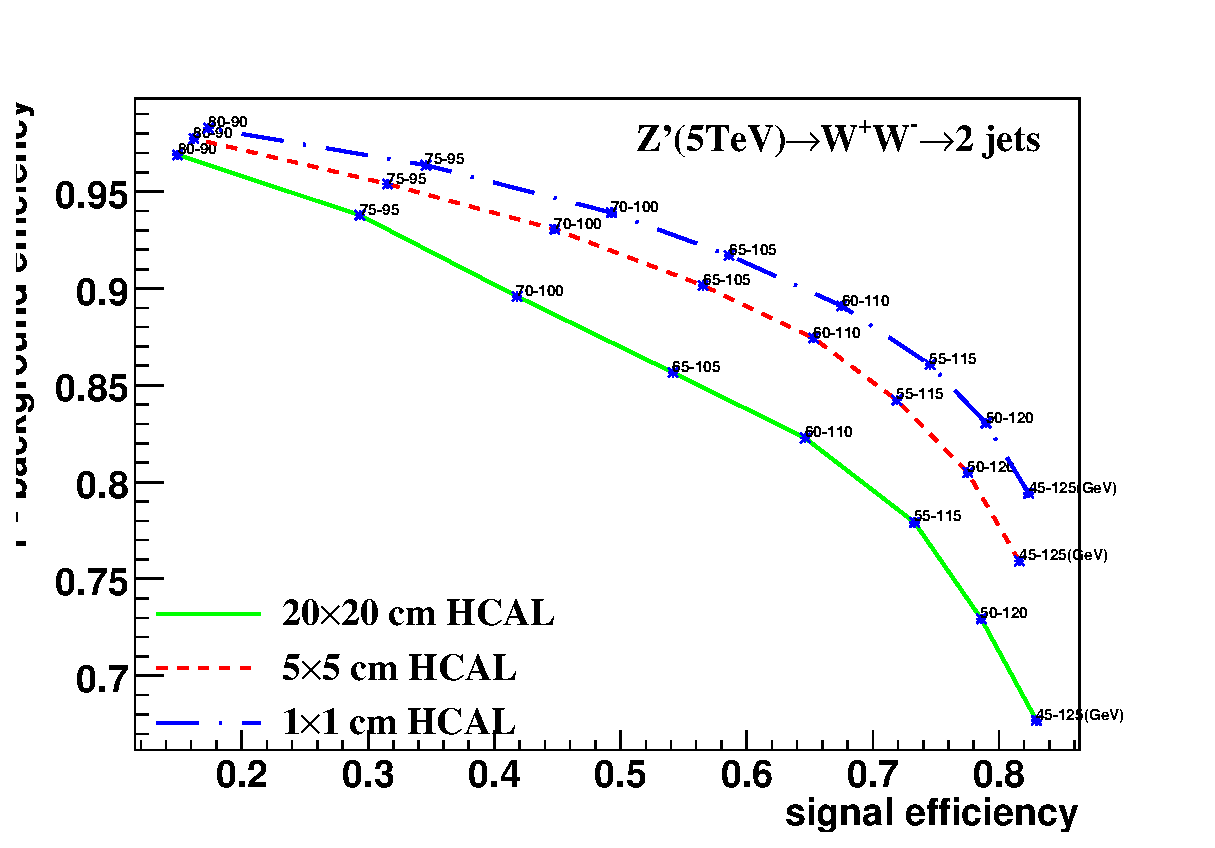
\includegraphics[width=0.43\textwidth]{figs/A_Cluster_mass_mmdt_5tev_eff_1_central_fix_at_85GeV_ww_qq.eps}
   }
   \subfigure[Central at 90TeV change width in cluster] {
   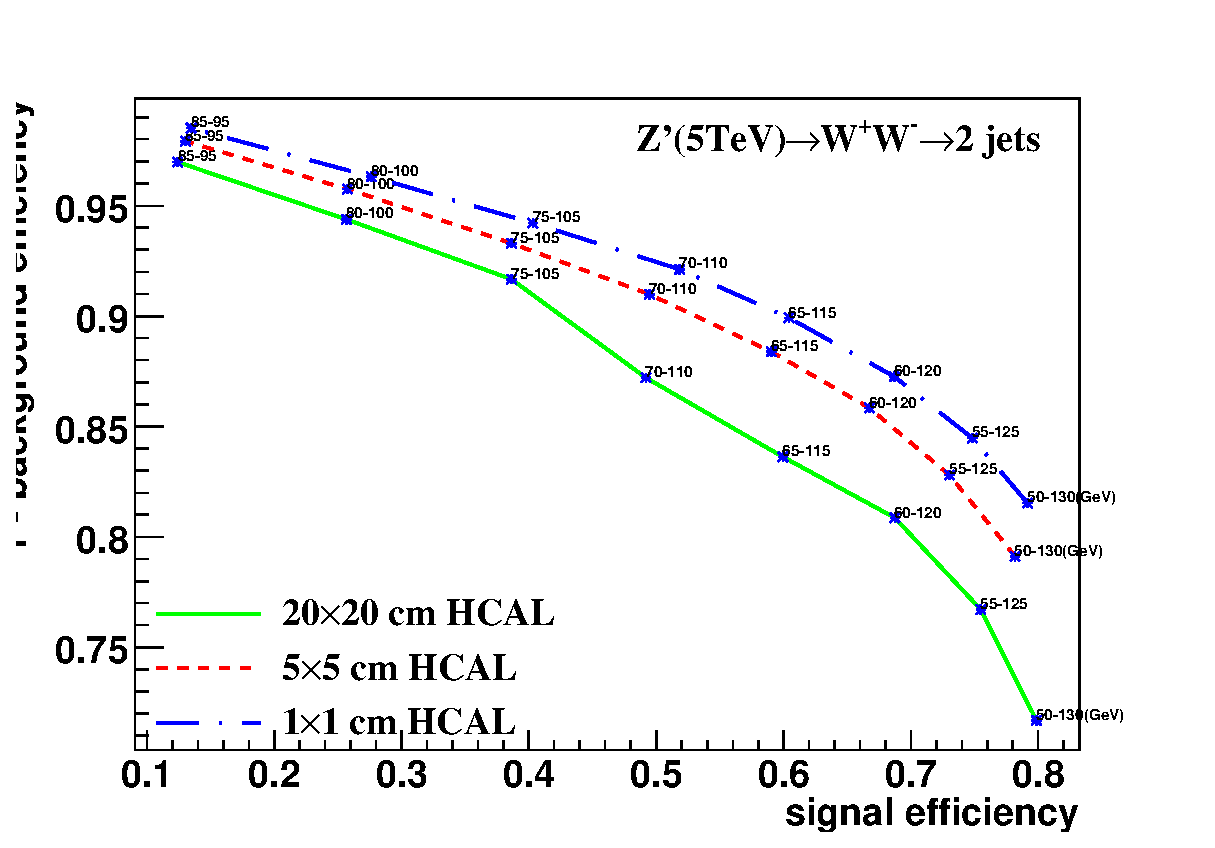
\includegraphics[width=0.43\textwidth]{figs/A_Cluster_mass_mmdt_5tev_eff_1_central_fix_at_90GeV_ww_qq.eps}
   }
   \subfigure[Central at 95TeV change width in cluster] {
   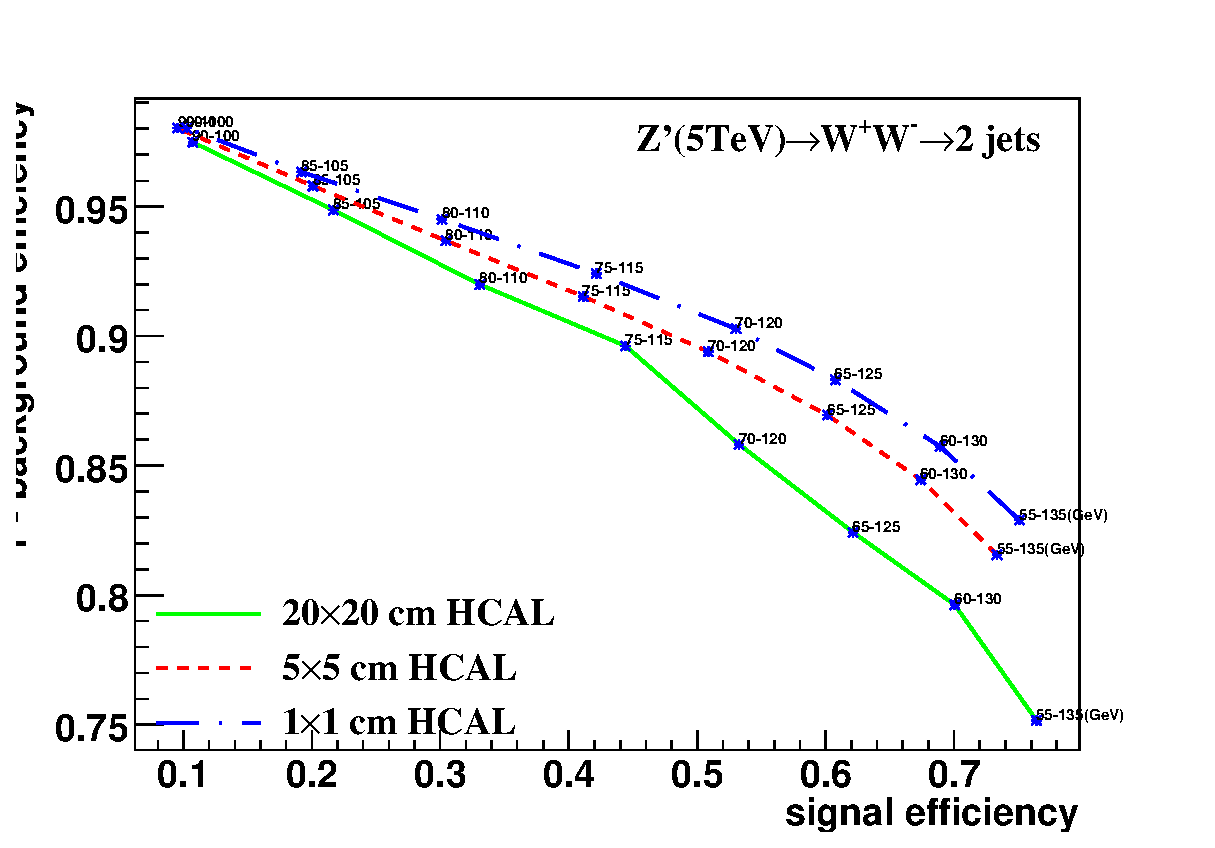
\includegraphics[width=0.43\textwidth]{figs/A_Cluster_mass_mmdt_5tev_eff_1_central_fix_at_95GeV_ww_qq.eps}
   }
   %\subfigure[Central at 100TeV change width in cluster] {
   %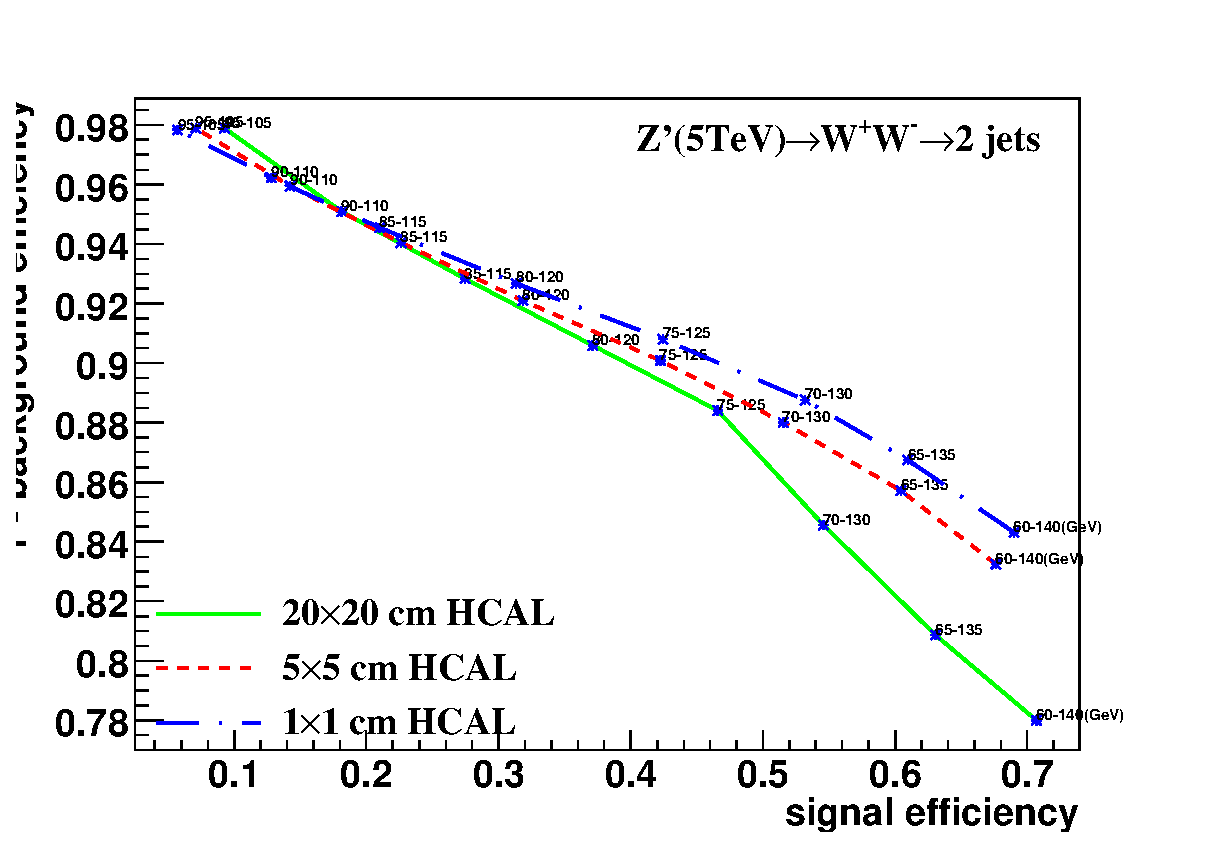
\includegraphics[width=0.43\textwidth]{figs/A_Cluster_mass_mmdt_5tev_eff_1_central_fix_at_100GeV_ww_qq.eps}
   %}
\end{center}
\caption{study of "fix central and change width" in mass soft drop at $\beta$=0, signal=ww, in 5TeV energy of collision  in different detector sizes. Cell Size in 20$\times$20, 5$\times$5, and 1$\times$1(cm$\times$cm) are shown in each picture.}
\label{fig:cluster_tau21_tau32}
\end{figure}

%50bins
\begin{figure}
\begin{center}
   \subfigure[10TeV at 20$\times$20(cm$\times$cm) in cluster] {
   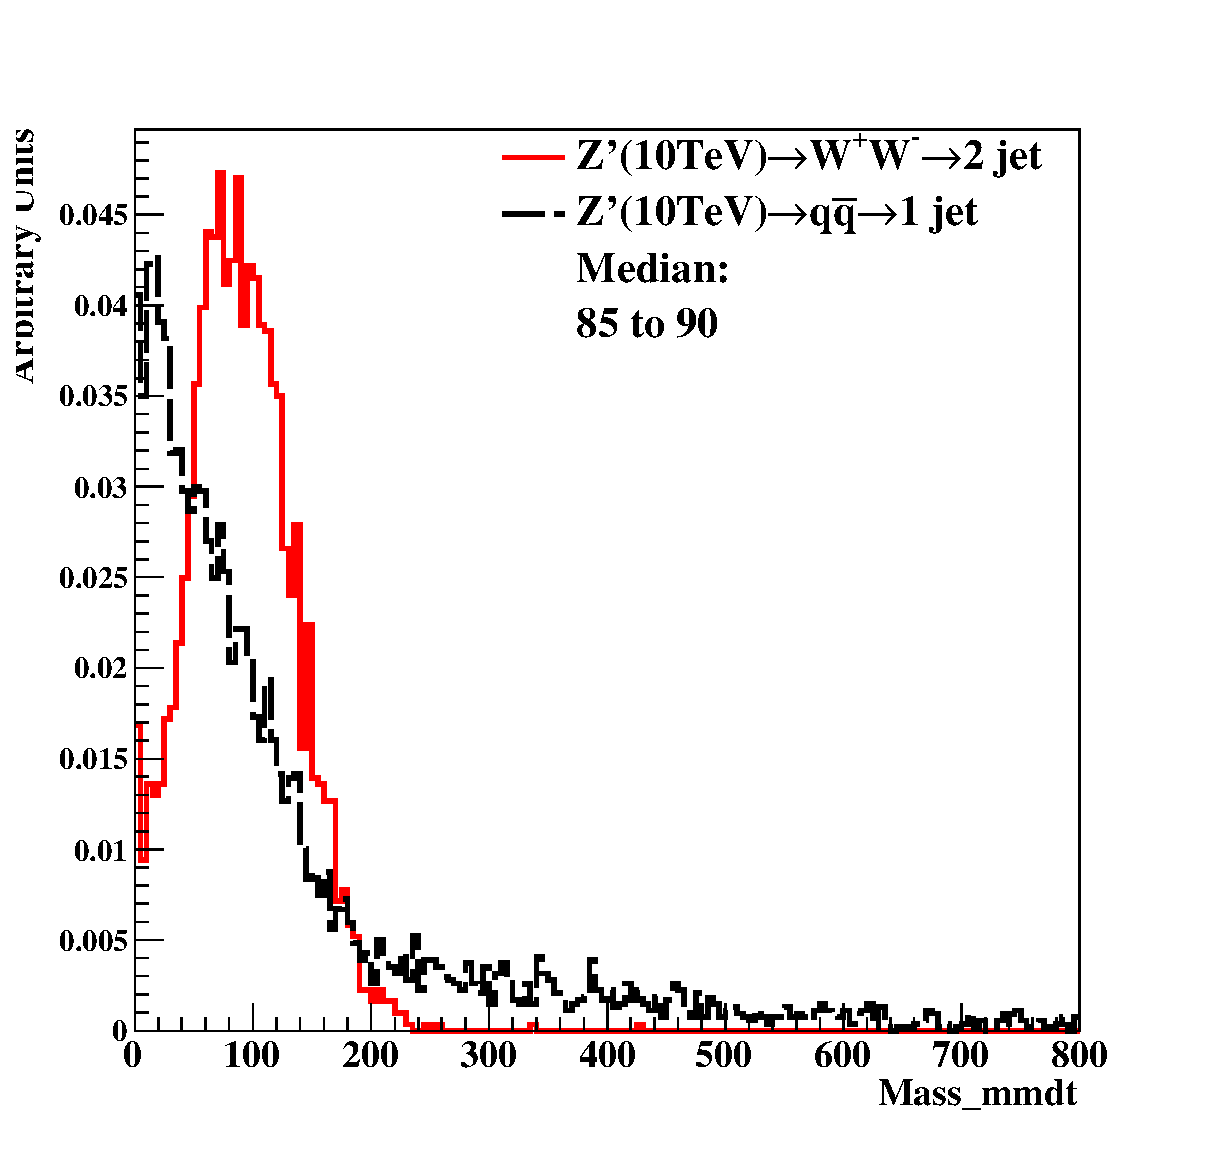
\includegraphics[width=0.43\textwidth]{figs/Dis_cluster_010_mass_mmdt_10tev_04.eps}\hfill
   }
   \subfigure[10TeV at 5$\times$5(cm$\times$cm) in cluster] {
   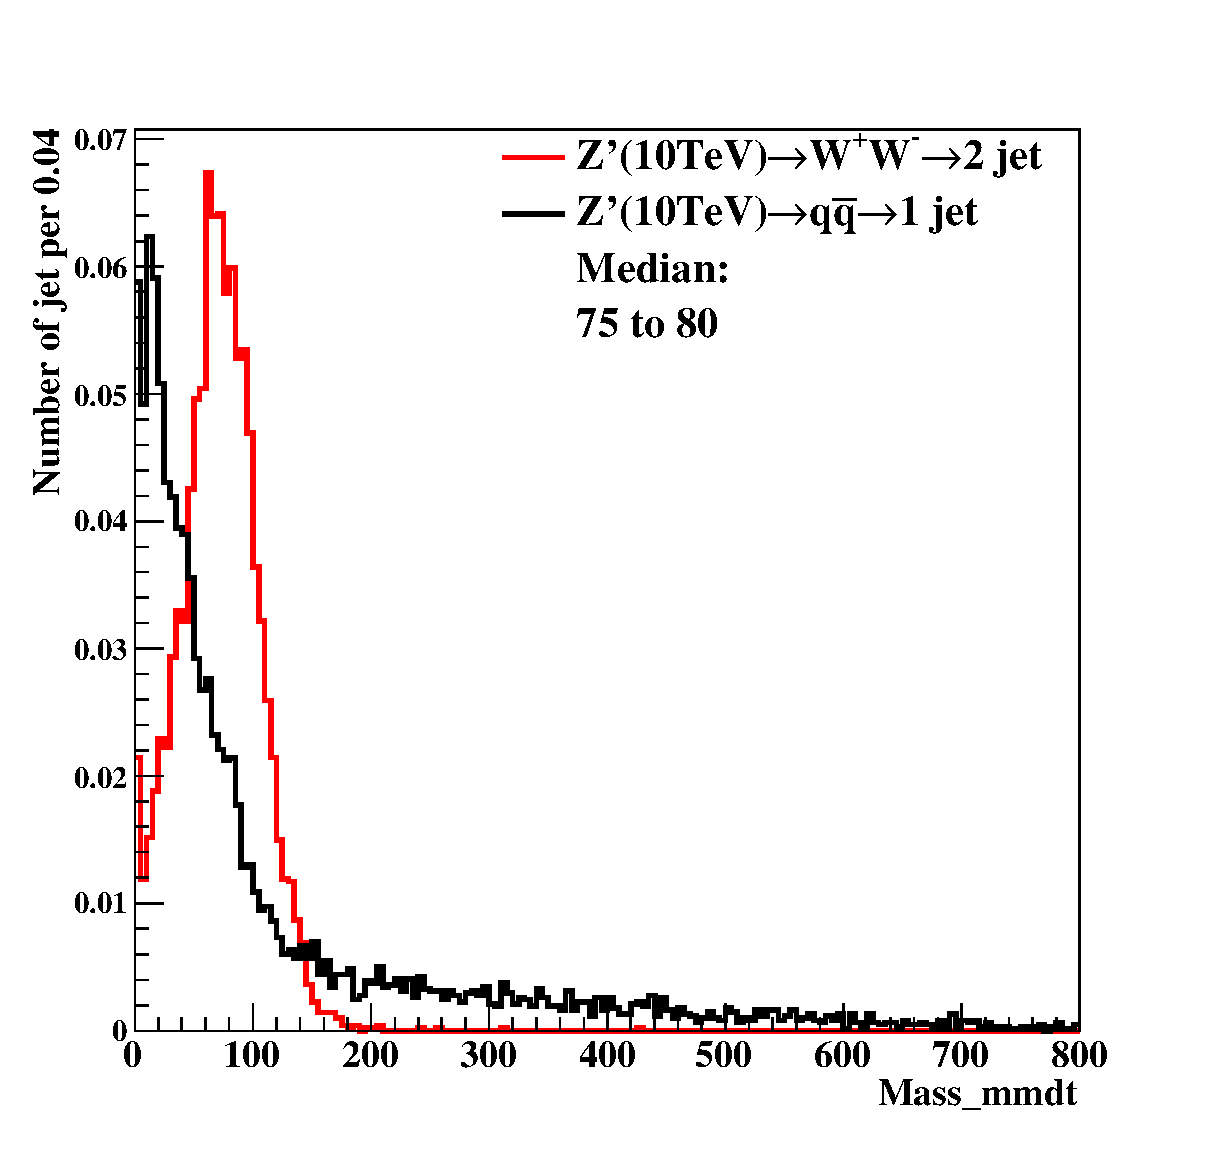
\includegraphics[width=0.43\textwidth]{figs/Dis_cluster_009_mass_mmdt_10tev_04.eps}
   }
   \subfigure[10TeV at 1$\times$1(cm$\times$cm) in cluster] {
   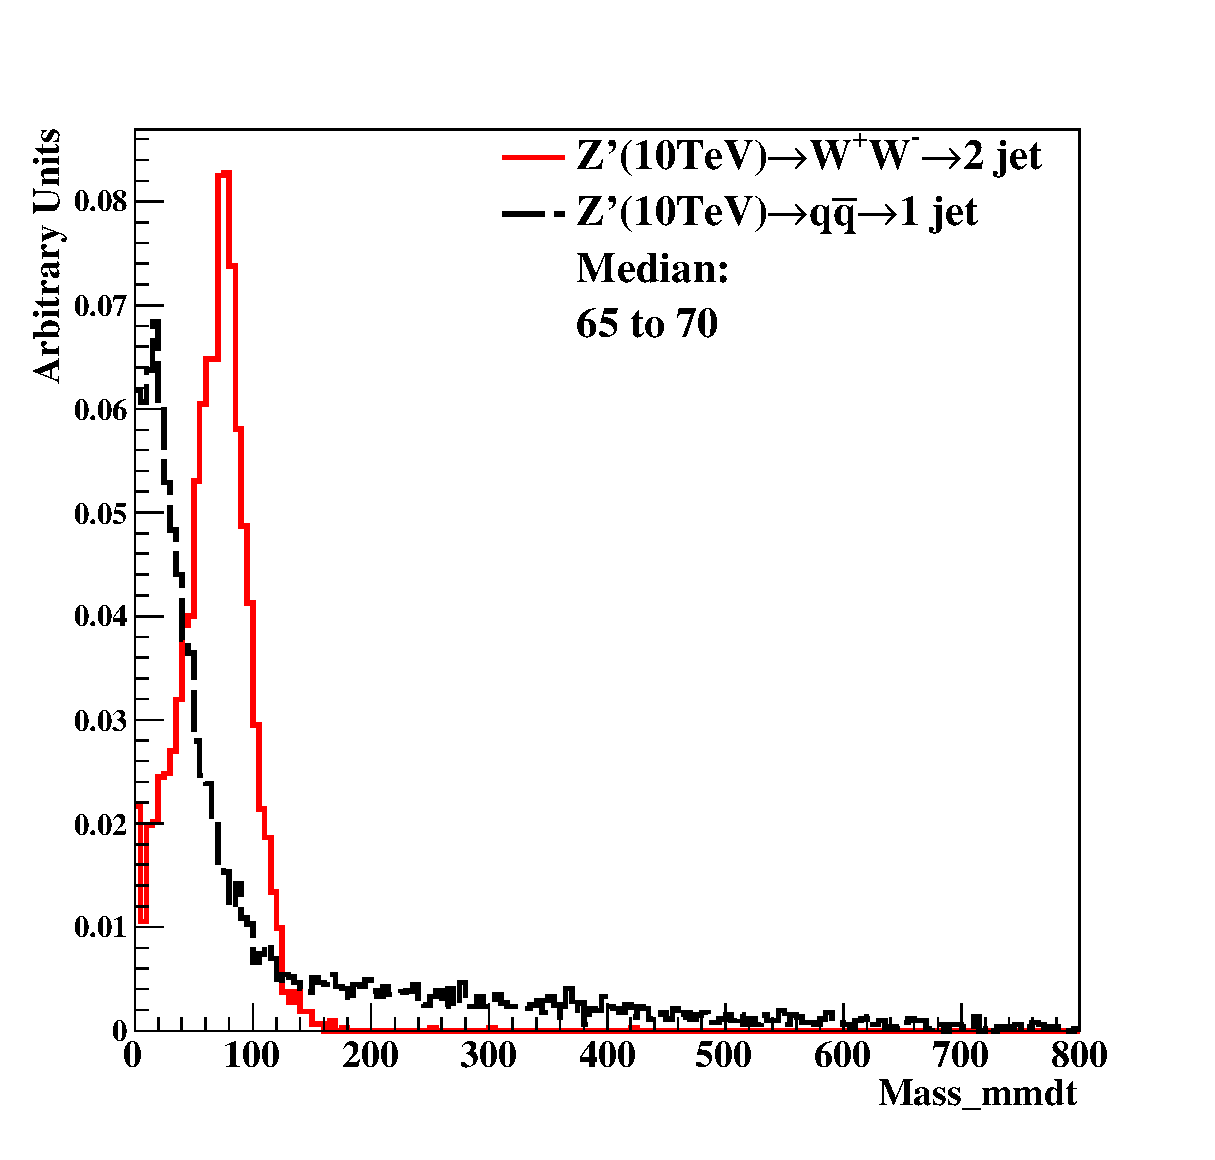
\includegraphics[width=0.43\textwidth]{figs/Dis_cluster_012_mass_mmdt_10tev_04.eps}
   }

\end{center}
\caption{Distributions of mass soft drop at $\beta$=0, signal=ww, in 10TeV energy of collision  in different detector sizes. Cell Size in 20$\times$20, 5$\times$5, and 1$\times$1(cm$\times$cm) are shown here.}
\label{fig:cluster_tau21_tau32}
\end{figure}

\begin{figure}
\begin{center}
   \subfigure[Central at 60TeV change width in cluster ] {
   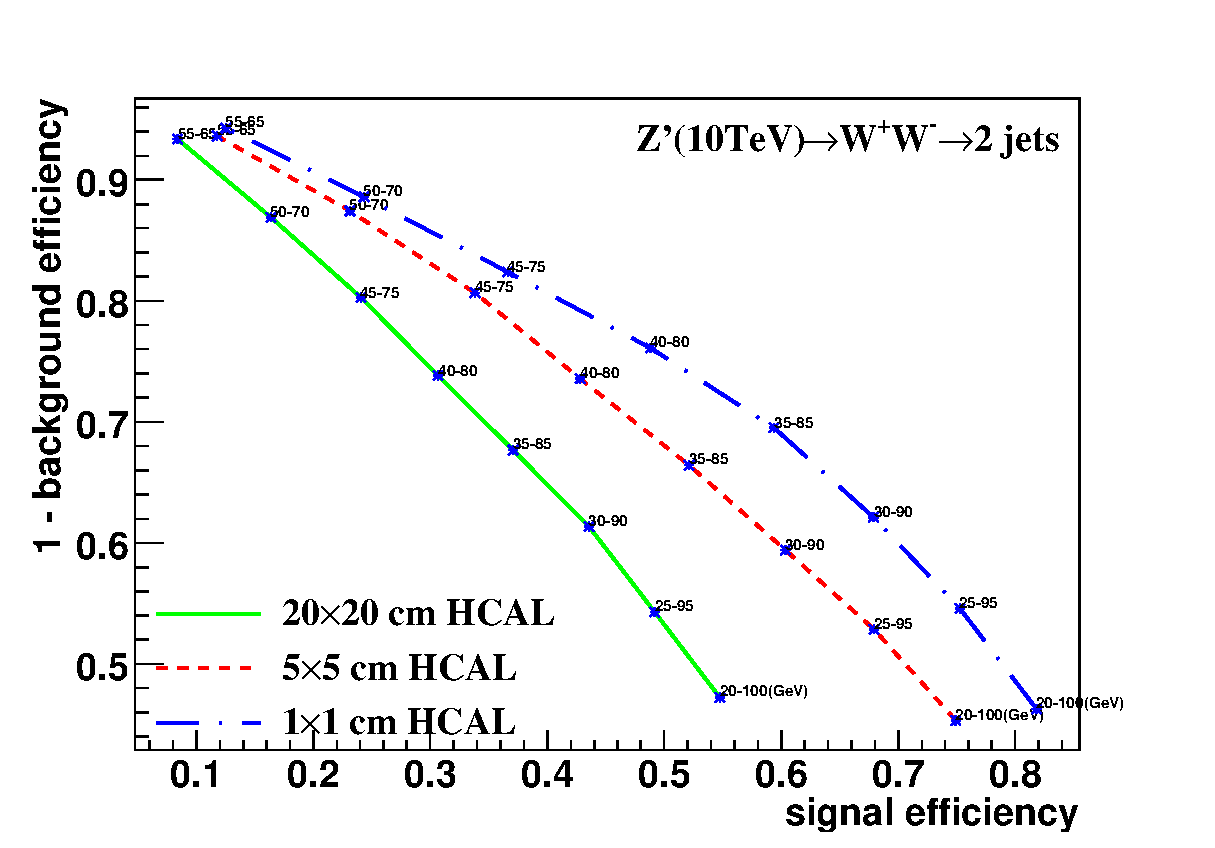
\includegraphics[width=0.43\textwidth]{figs/A_Cluster_mass_mmdt_10tev_eff_1_central_fix_at_60GeV_ww_qq.eps}\hfill
   }
   \subfigure[Central at 65TeV change width in cluster] {
   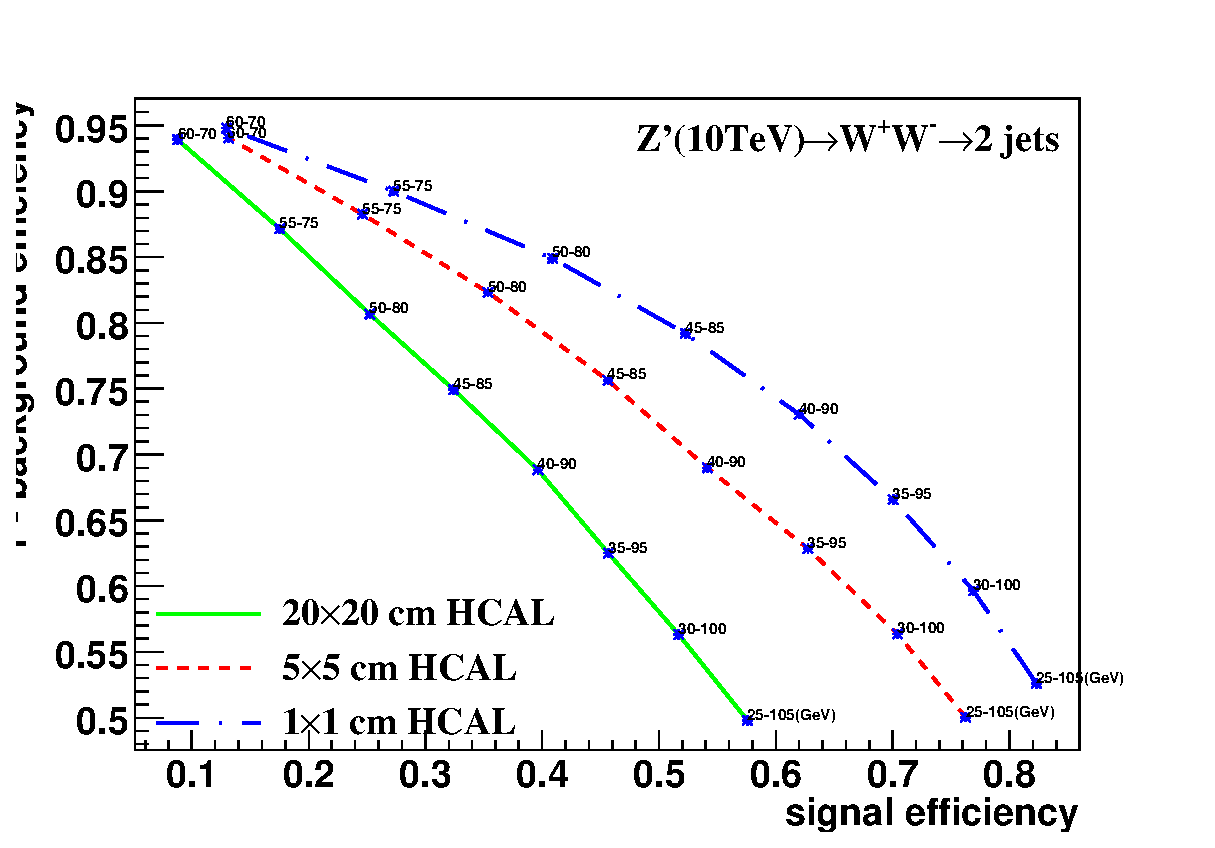
\includegraphics[width=0.43\textwidth]{figs/A_Cluster_mass_mmdt_10tev_eff_1_central_fix_at_65GeV_ww_qq.eps}
   }
   \subfigure[Central at 70TeV change width in cluster] {
   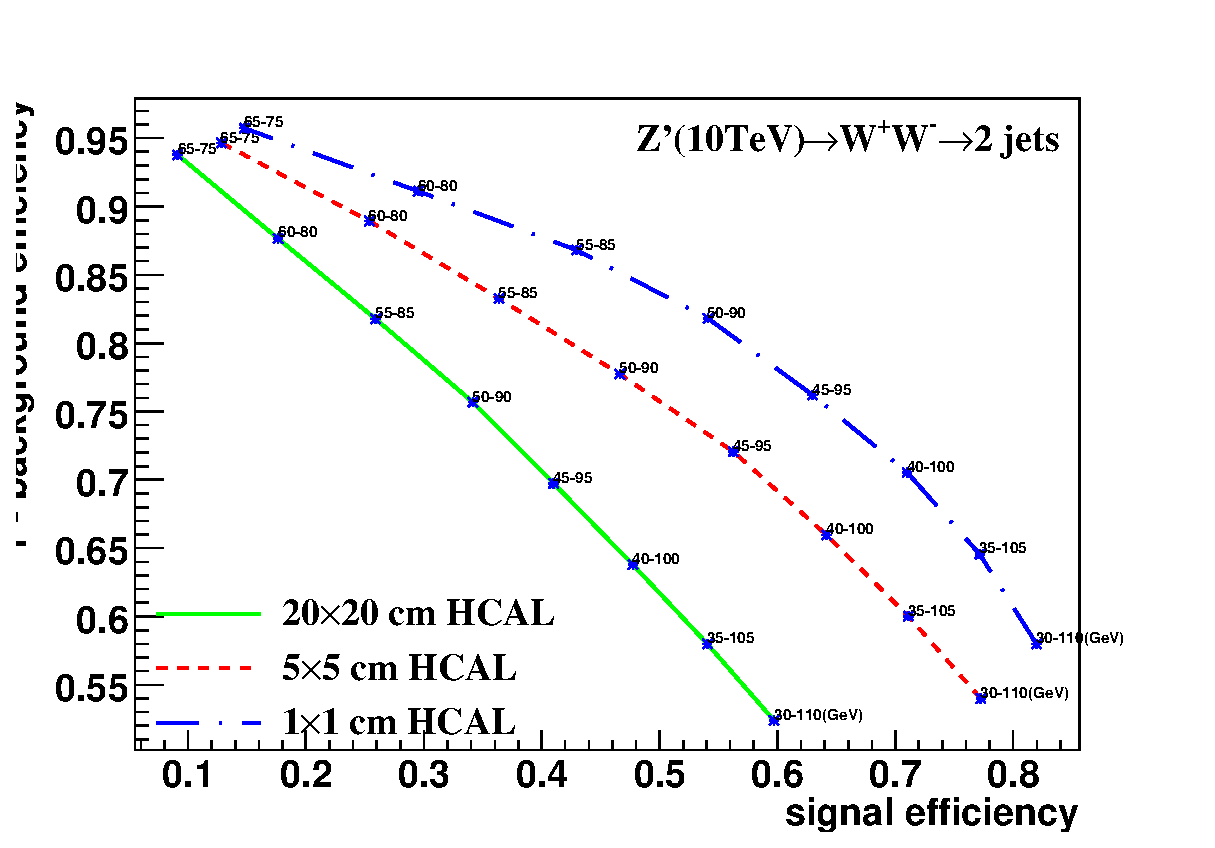
\includegraphics[width=0.43\textwidth]{figs/A_Cluster_mass_mmdt_10tev_eff_1_central_fix_at_70GeV_ww_qq.eps}
   }
   \subfigure[Central at 75TeV change width in cluster] {
   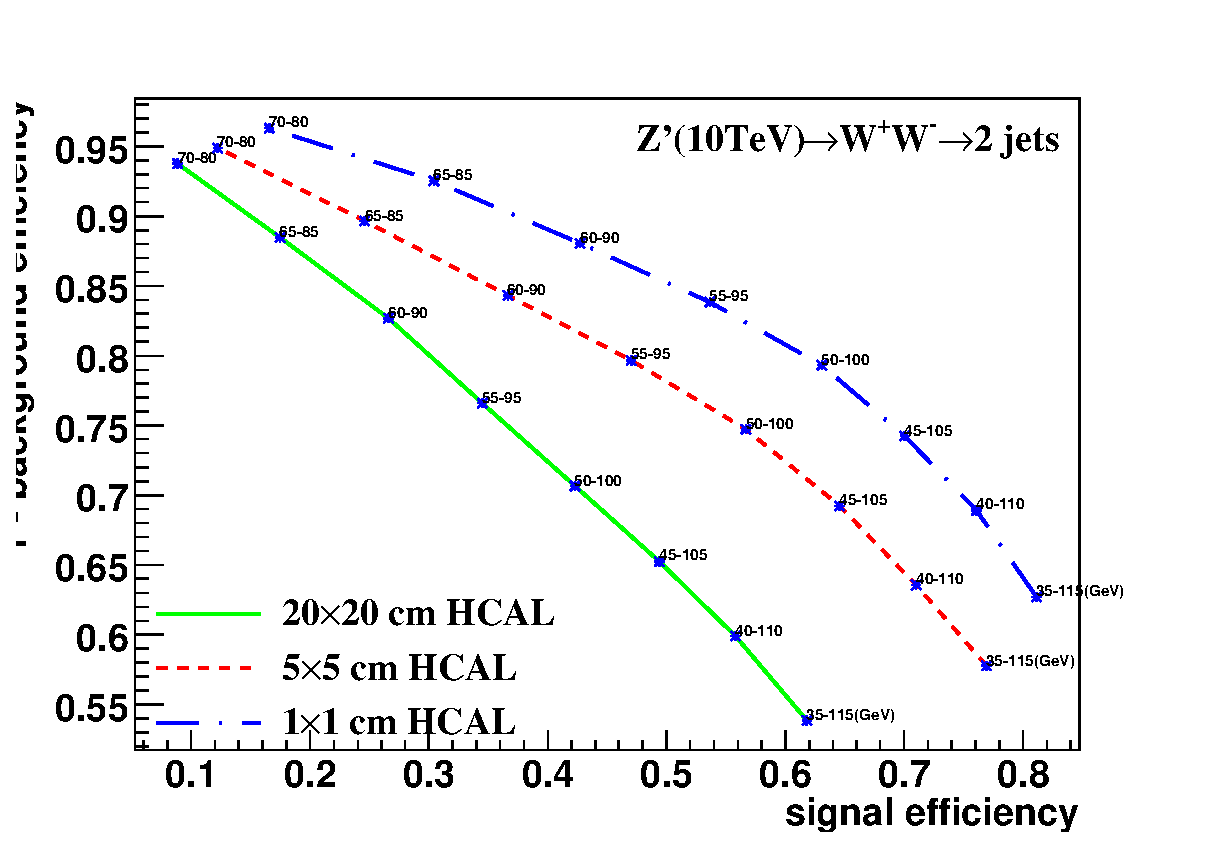
\includegraphics[width=0.43\textwidth]{figs/A_Cluster_mass_mmdt_10tev_eff_1_central_fix_at_75GeV_ww_qq.eps}
   }
   \subfigure[Central at 80TeV change width in cluster] {
   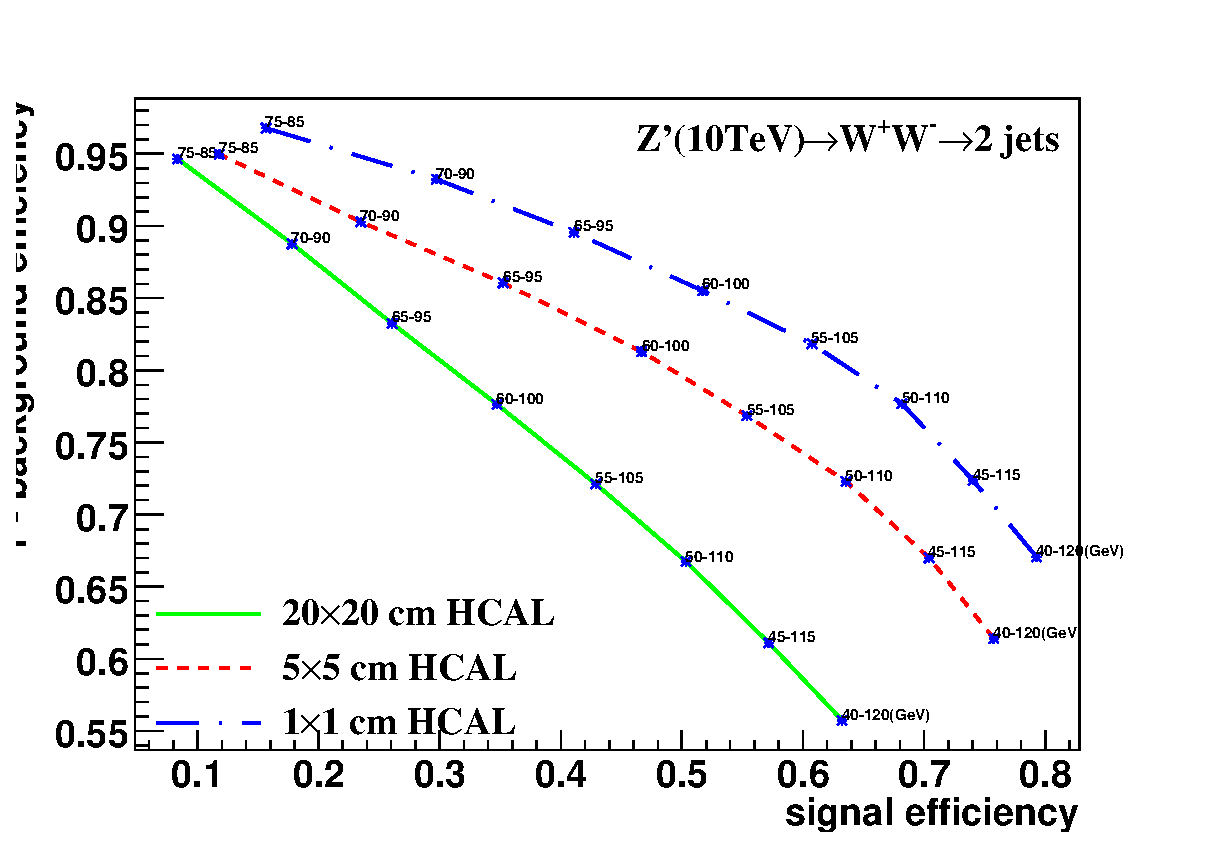
\includegraphics[width=0.43\textwidth]{figs/A_Cluster_mass_mmdt_10tev_eff_1_central_fix_at_80GeV_ww_qq.eps}
   }
   \subfigure[Central at 85TeV change width in cluster] {
   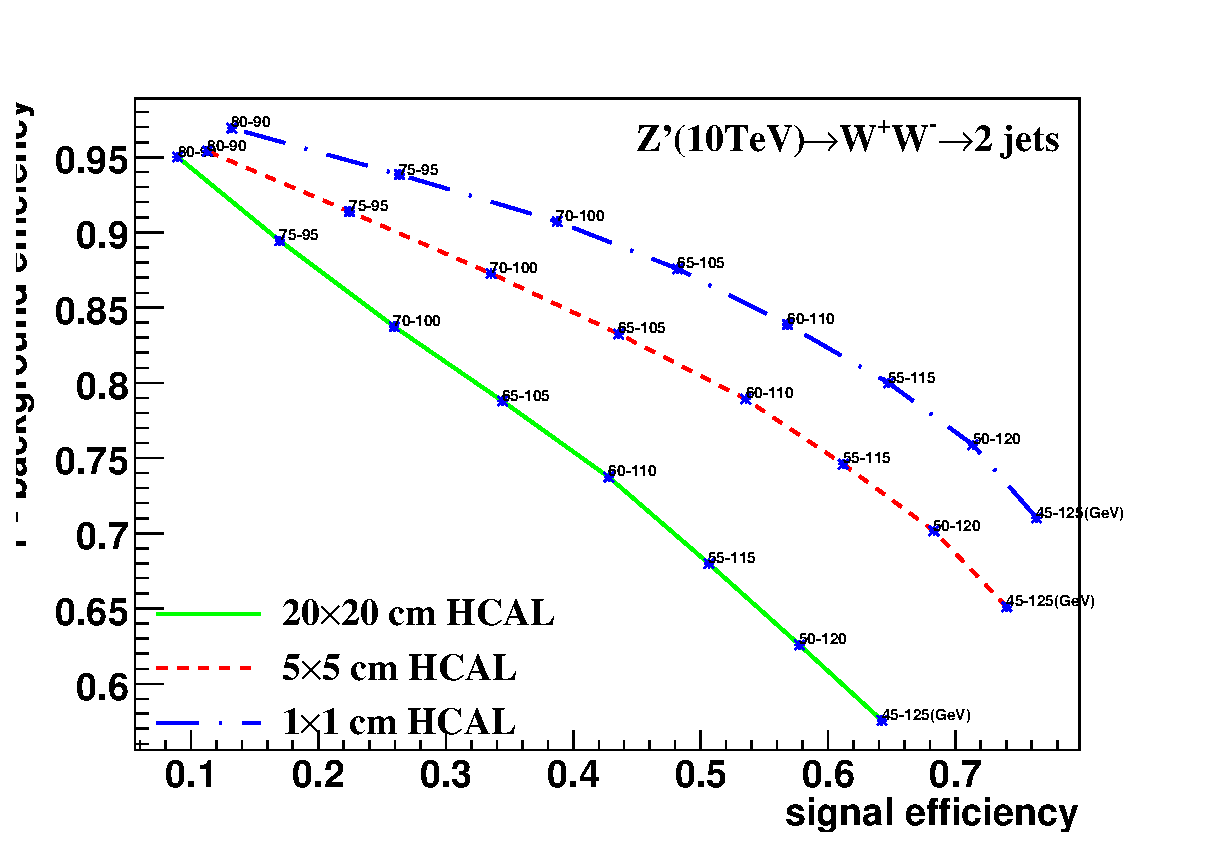
\includegraphics[width=0.43\textwidth]{figs/A_Cluster_mass_mmdt_10tev_eff_1_central_fix_at_85GeV_ww_qq.eps}
   }
   \subfigure[Central at 90TeV change width in cluster] {
   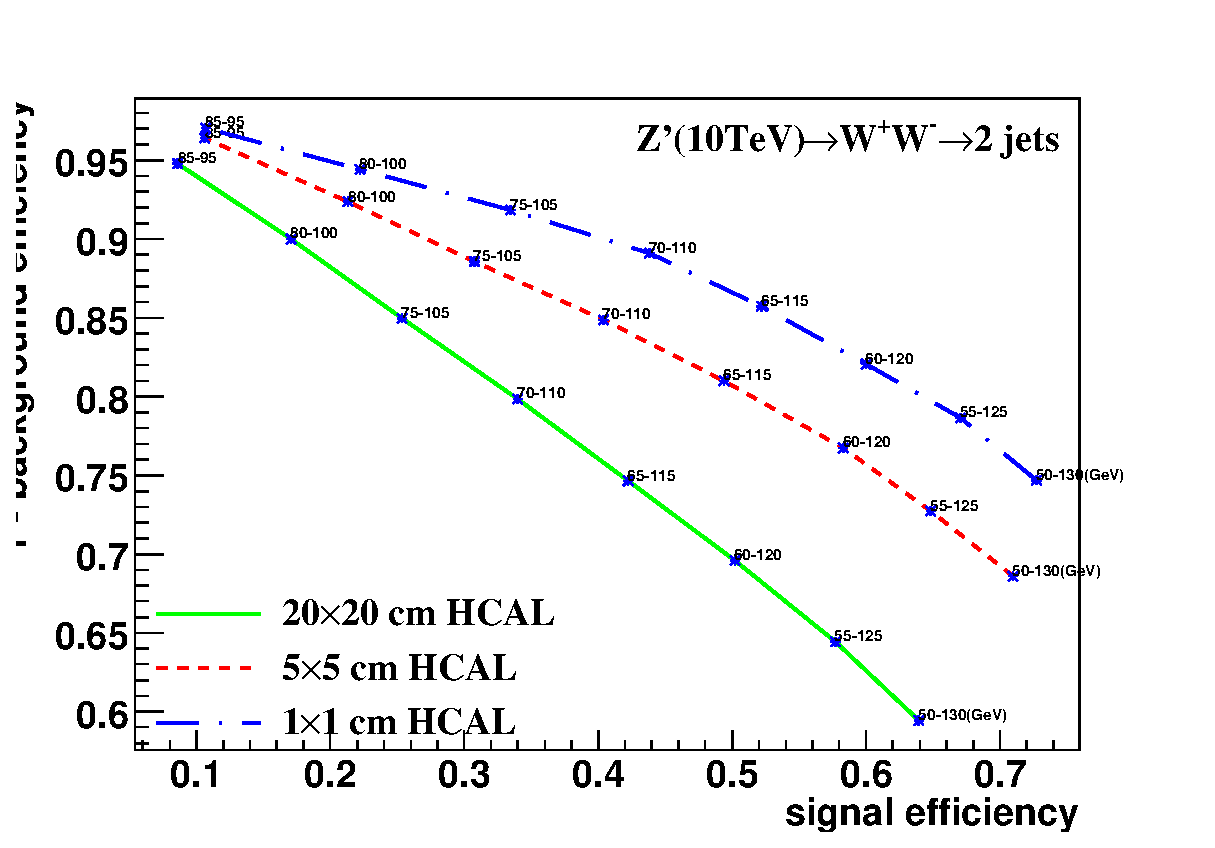
\includegraphics[width=0.43\textwidth]{figs/A_Cluster_mass_mmdt_10tev_eff_1_central_fix_at_90GeV_ww_qq.eps}
   }
   \subfigure[Central at 95TeV change width in cluster] {
   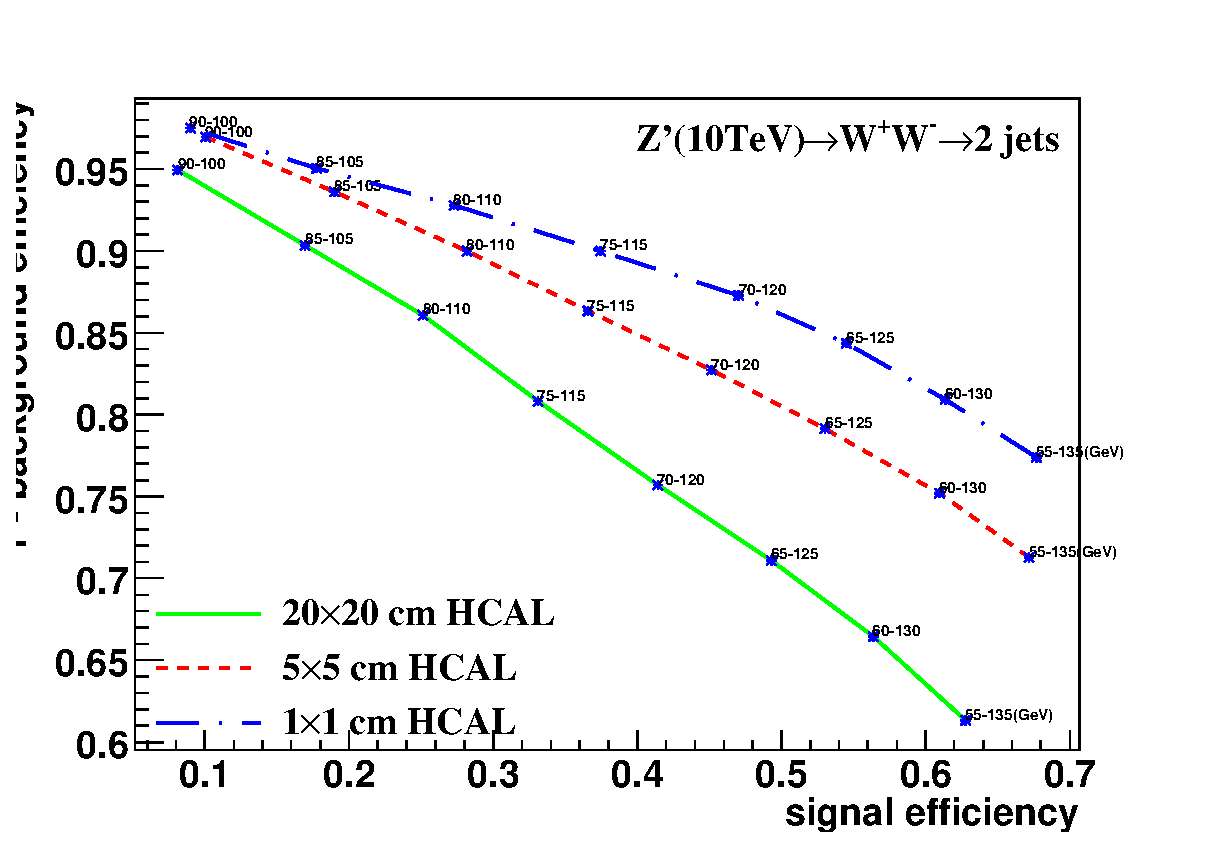
\includegraphics[width=0.43\textwidth]{figs/A_Cluster_mass_mmdt_10tev_eff_1_central_fix_at_95GeV_ww_qq.eps}
   }
   %\subfigure[Central at 100TeV change width in cluster] {
   %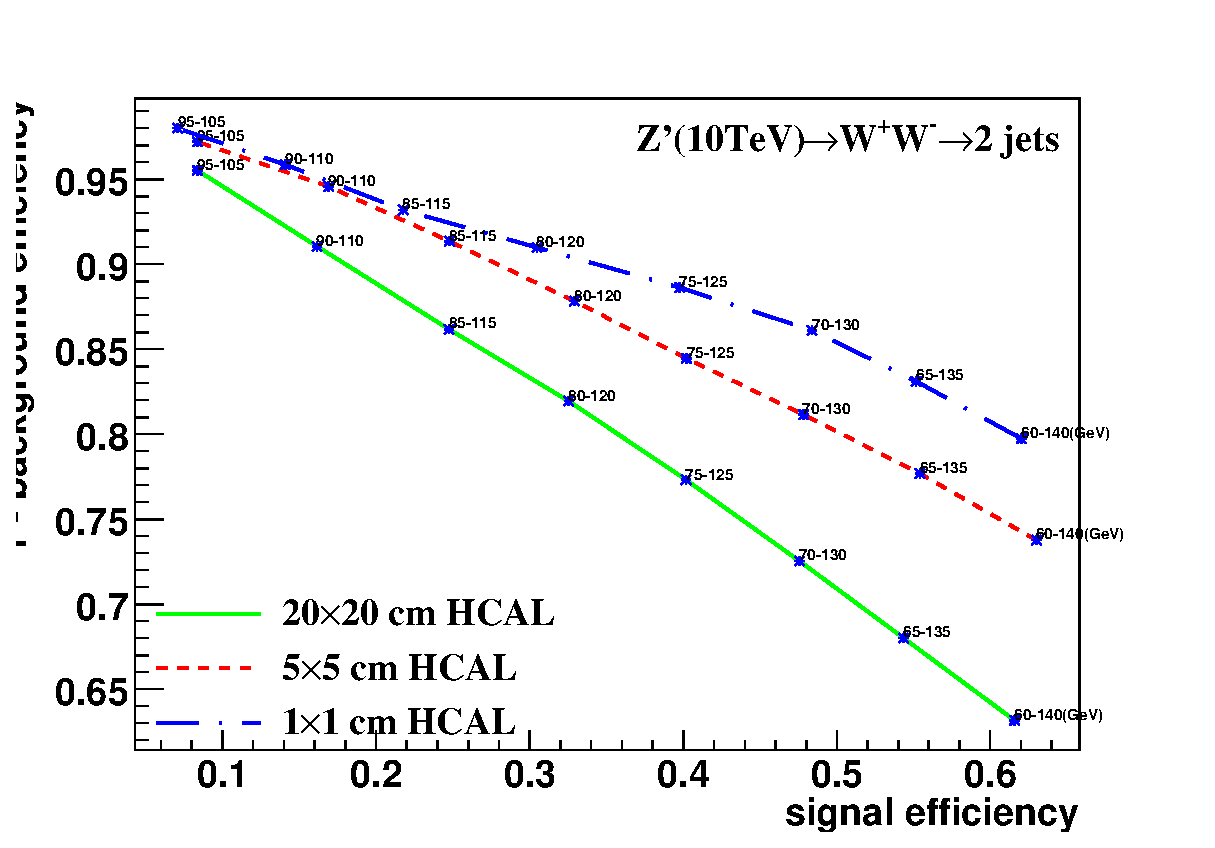
\includegraphics[width=0.43\textwidth]{figs/A_Cluster_mass_mmdt_10tev_eff_1_central_fix_at_100GeV_ww_qq.eps}
   %}


\end{center}
\caption{study of "fix central and change width" in mass soft drop at $\beta$=0, signal=ww, in 10TeV energy of collision  in different detector sizes. Cell Size in 20$\times$20, 5$\times$5, and 1$\times$1(cm$\times$cm) are shown in each picture.}
\label{fig:cluster_tau21_tau32}
\end{figure}

%50bins
\begin{figure}
\begin{center}
   \subfigure[20TeV at 20$\times$20(cm$\times$cm) in cluster] {
   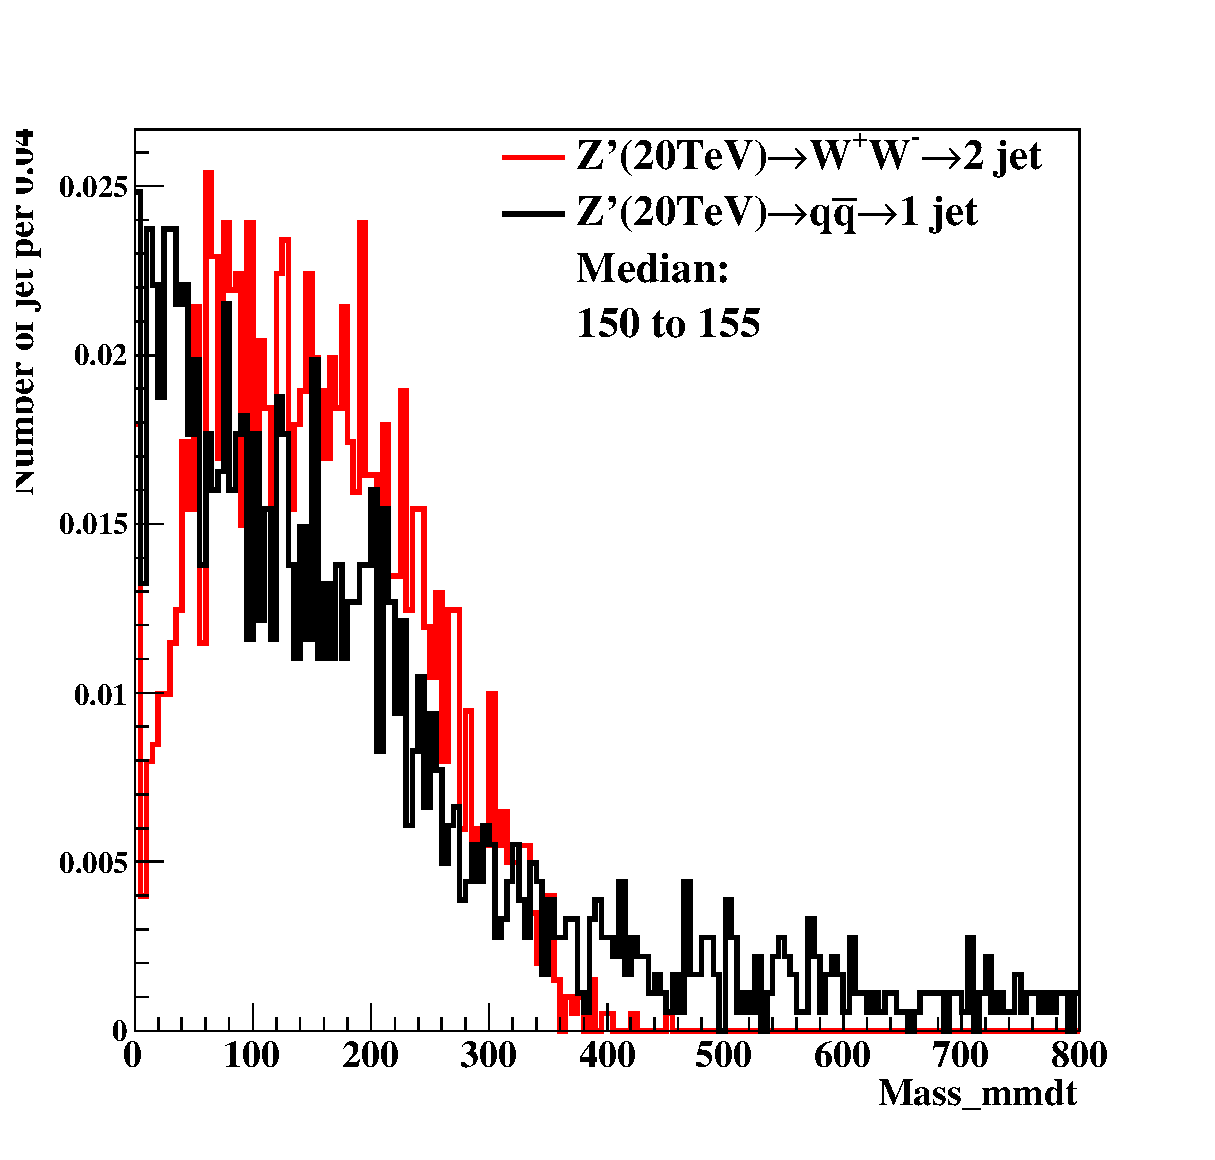
\includegraphics[width=0.43\textwidth]{figs/Dis_cluster_010_mass_mmdt_20tev_04.eps}\hfill
   }
   \subfigure[20TeV at 5$\times$5(cm$\times$cm) in cluster] {
   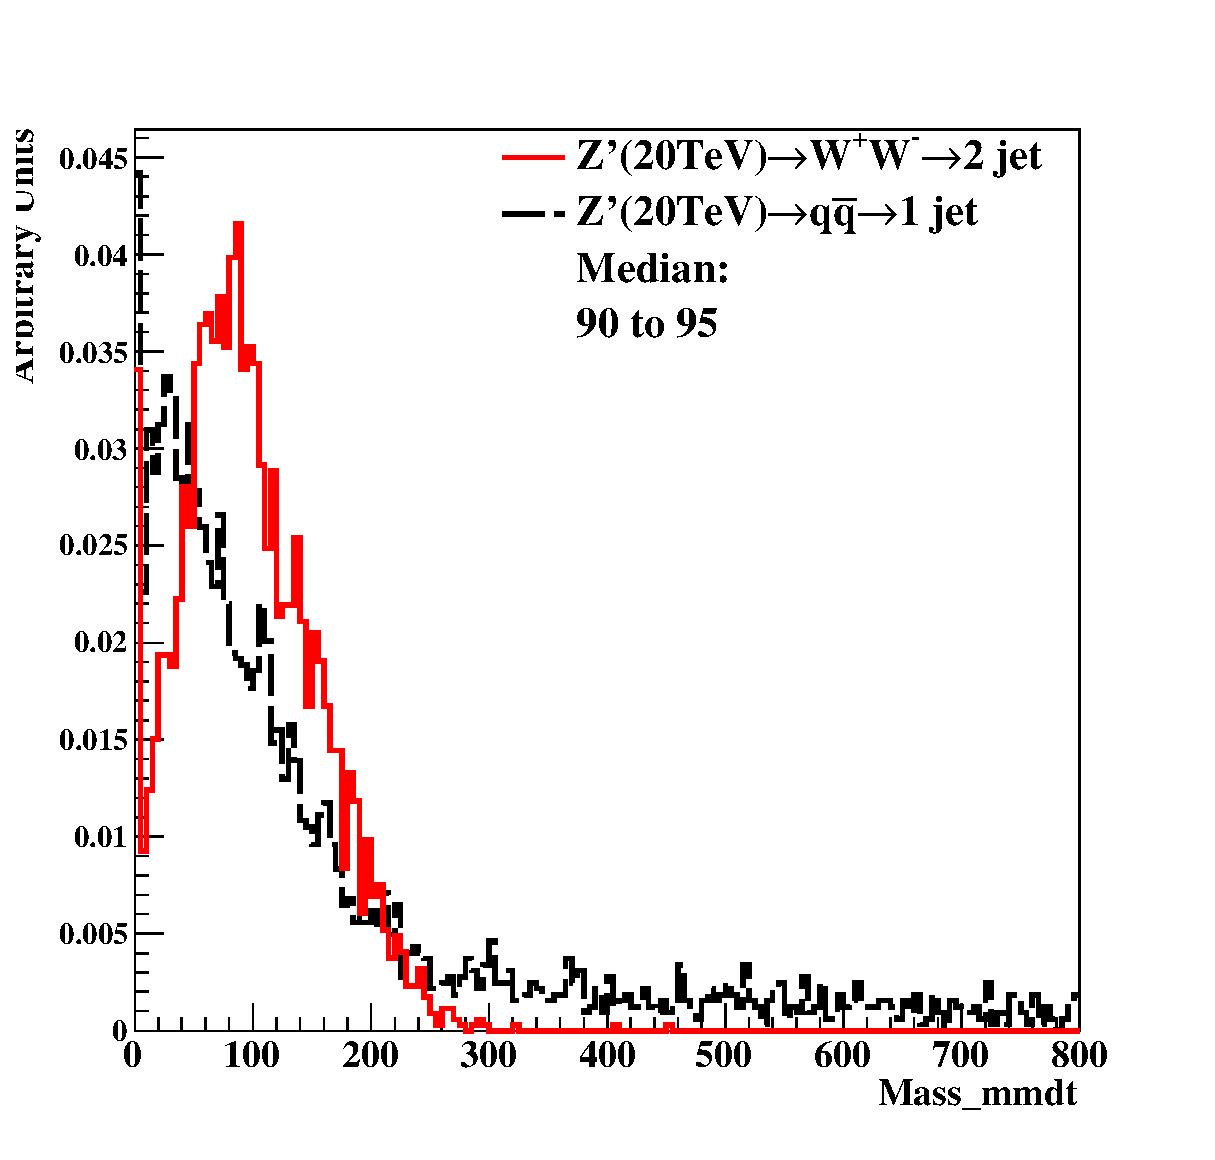
\includegraphics[width=0.43\textwidth]{figs/Dis_cluster_009_mass_mmdt_20tev_04.eps}
   }
   \subfigure[20TeV at 1$\times$1(cm$\times$cm) in cluster] {
   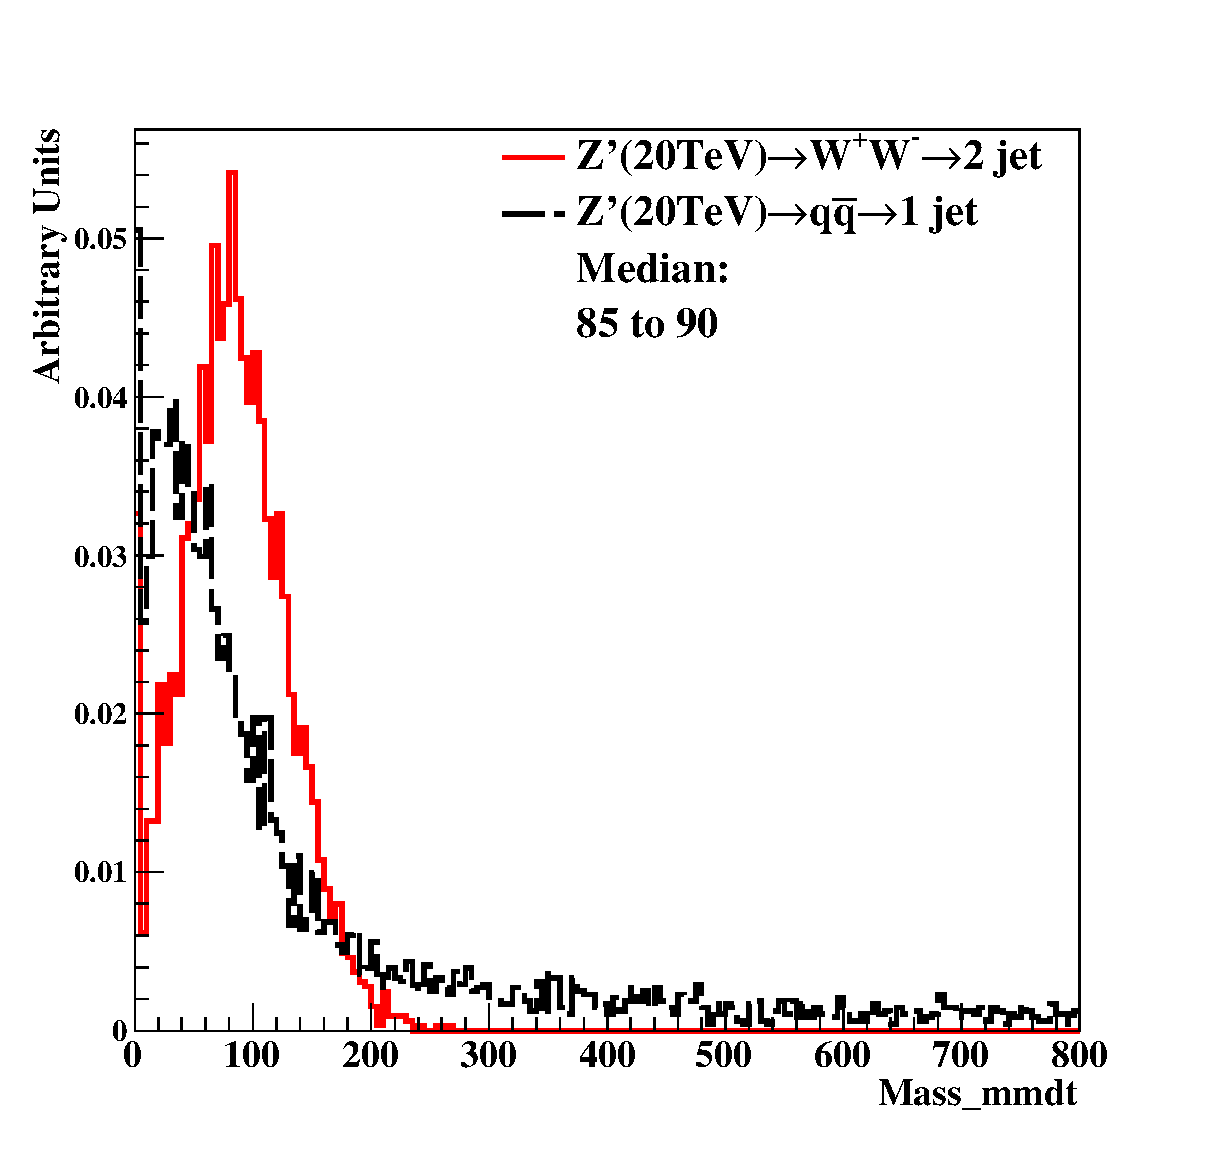
\includegraphics[width=0.43\textwidth]{figs/Dis_cluster_012_mass_mmdt_20tev_04.eps}
   }

\end{center}
\caption{Distributions of mass soft drop at $\beta$=0, signal=ww, in 20TeV energy of collision  in different detector sizes. Cell Size in 20$\times$20, 5$\times$5, and 1$\times$1(cm$\times$cm) are shown here.}
\label{fig:cluster_tau21_tau32}
\end{figure}

\begin{figure}
\begin{center}
   \subfigure[Central at 60TeV change width in cluster ] {
   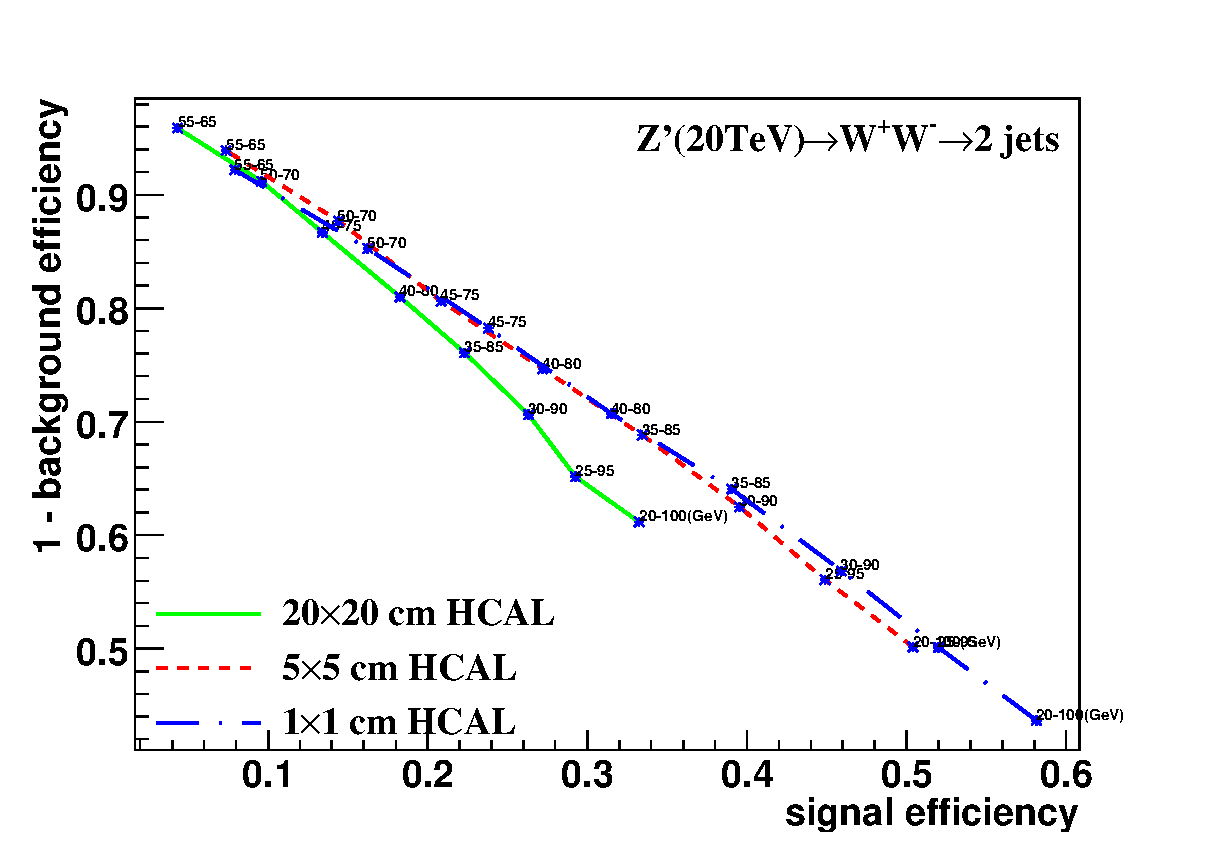
\includegraphics[width=0.43\textwidth]{figs/A_Cluster_mass_mmdt_20tev_eff_1_central_fix_at_60GeV_ww_qq.eps}\hfill
   }
   \subfigure[Central at 65TeV change width in cluster] {
   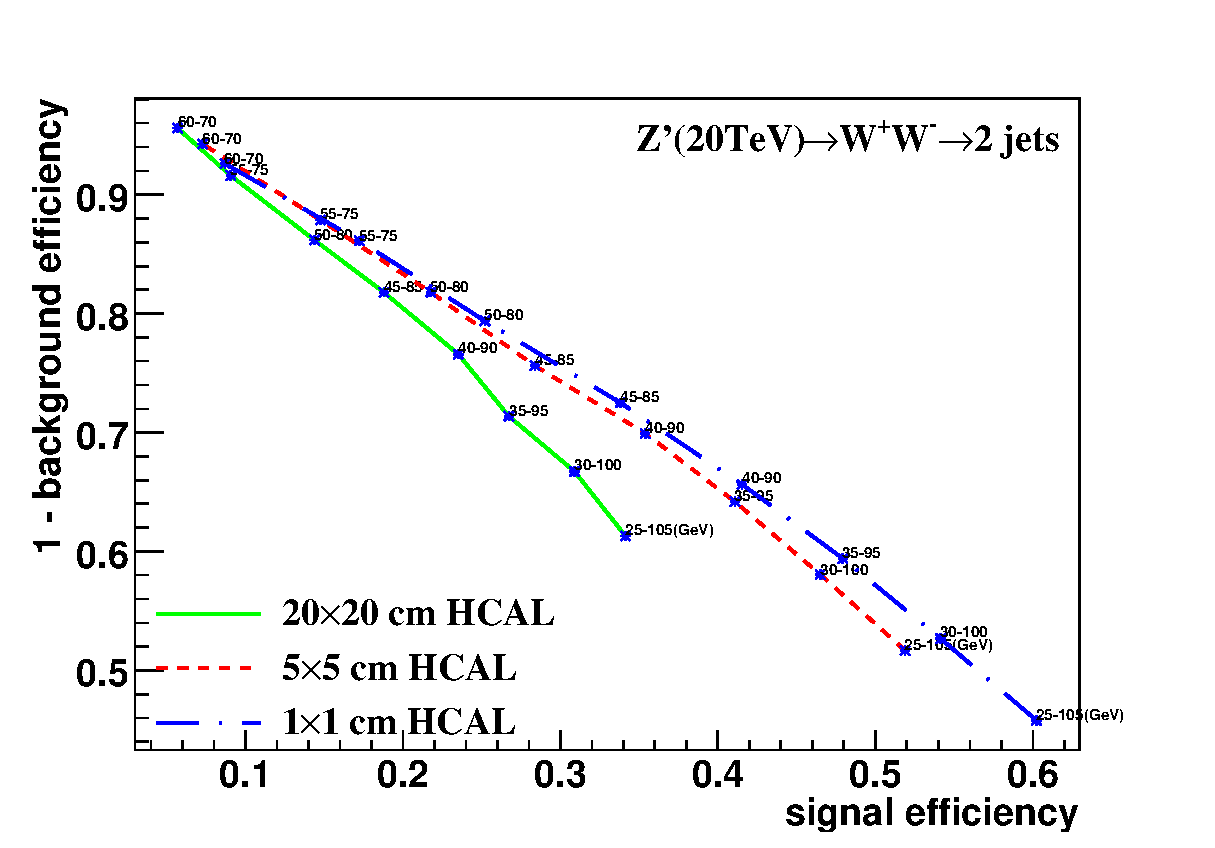
\includegraphics[width=0.43\textwidth]{figs/A_Cluster_mass_mmdt_20tev_eff_1_central_fix_at_65GeV_ww_qq.eps}
   }
   \subfigure[Central at 70TeV change width in cluster] {
   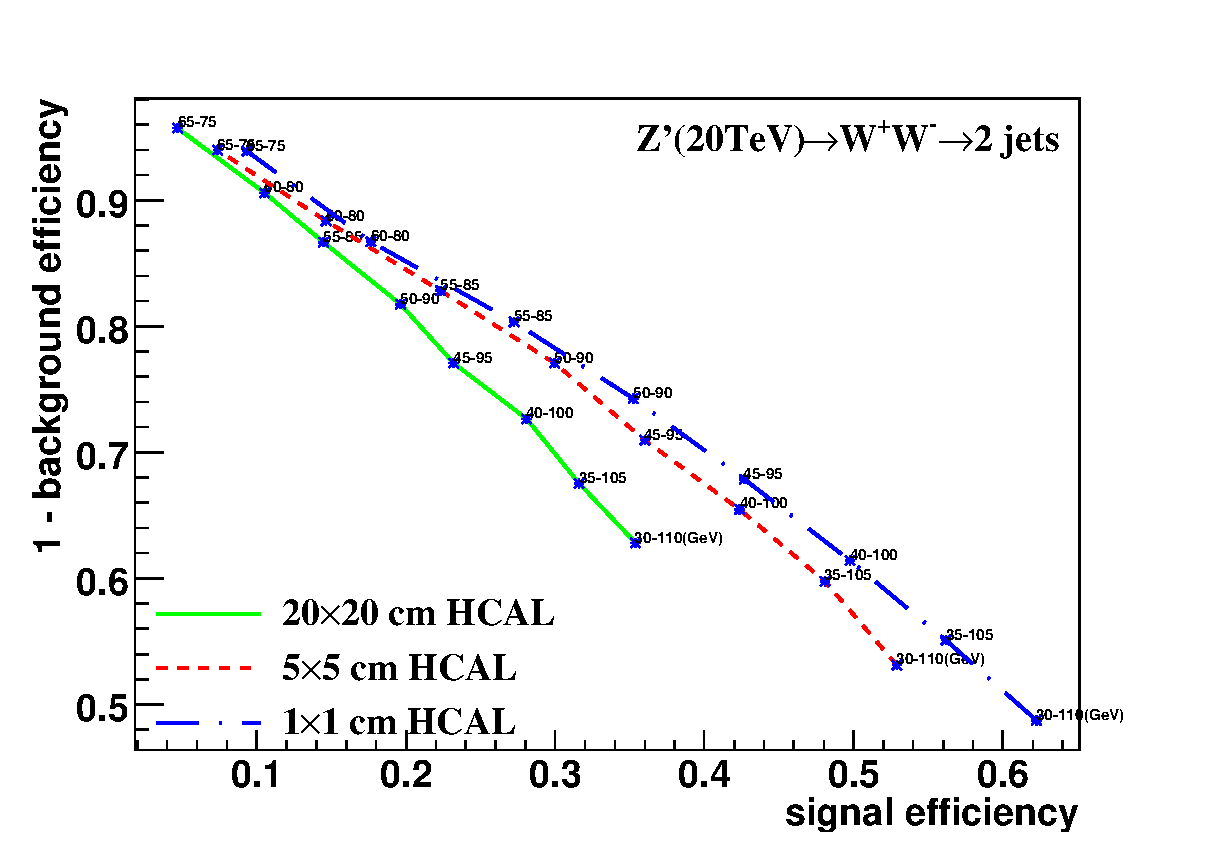
\includegraphics[width=0.43\textwidth]{figs/A_Cluster_mass_mmdt_20tev_eff_1_central_fix_at_70GeV_ww_qq.eps}
   }
   \subfigure[Central at 75TeV change width in cluster] {
   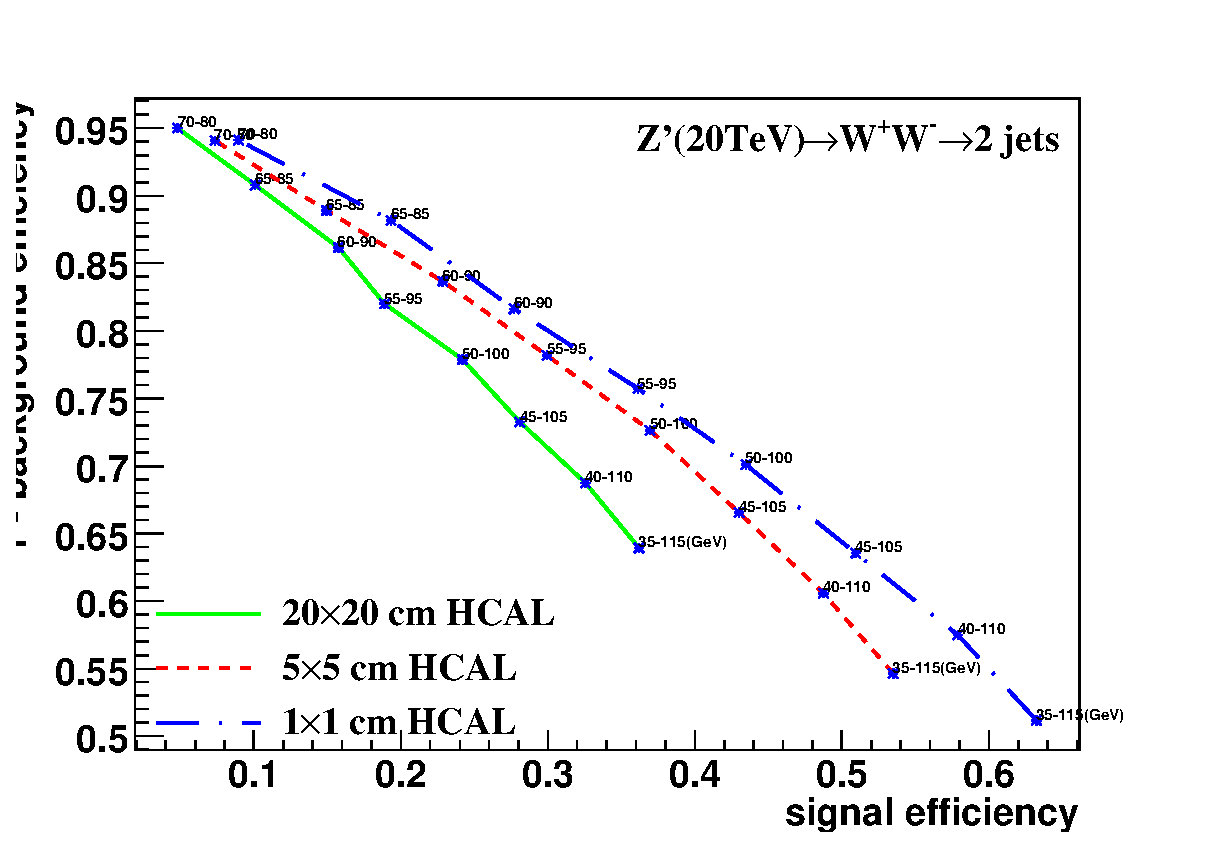
\includegraphics[width=0.43\textwidth]{figs/A_Cluster_mass_mmdt_20tev_eff_1_central_fix_at_75GeV_ww_qq.eps}
   }
   \subfigure[Central at 80TeV change width in cluster] {
   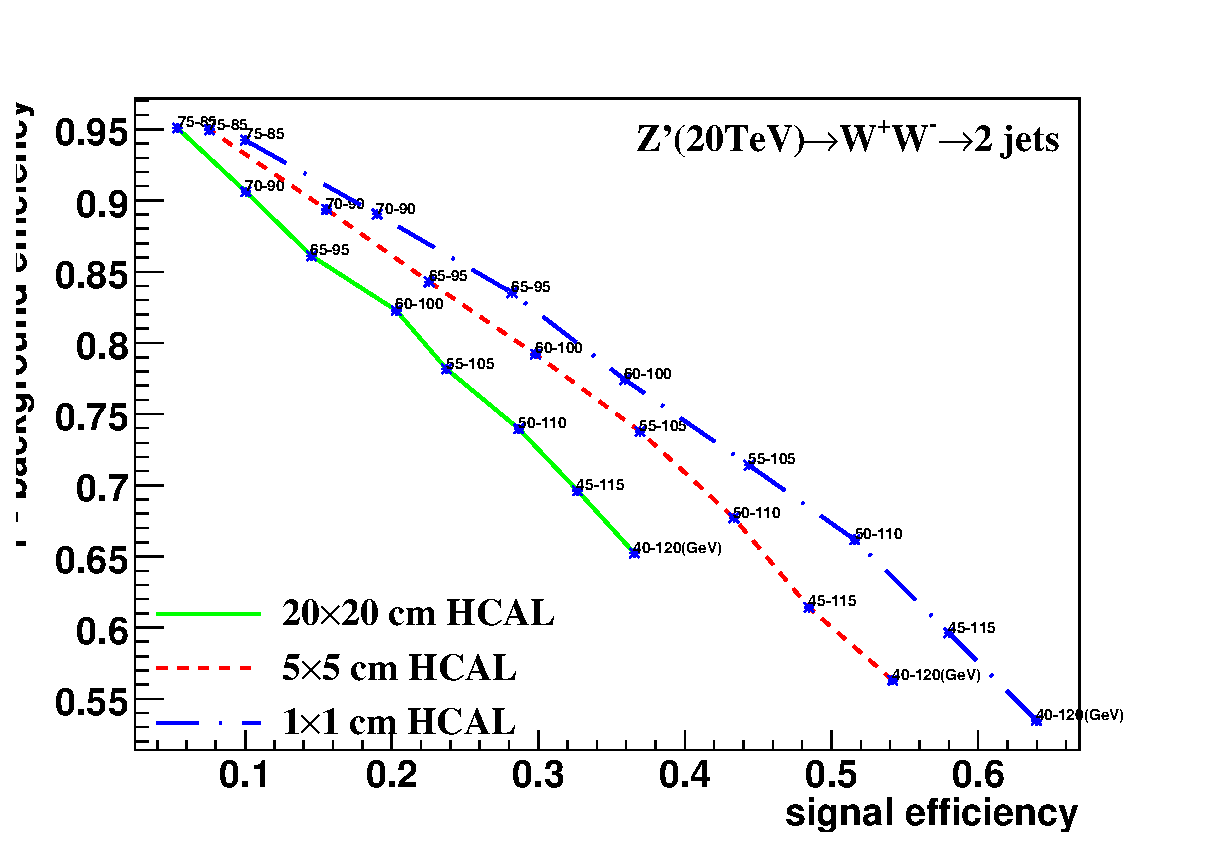
\includegraphics[width=0.43\textwidth]{figs/A_Cluster_mass_mmdt_20tev_eff_1_central_fix_at_80GeV_ww_qq.eps}
   }
   \subfigure[Central at 85TeV change width in cluster] {
   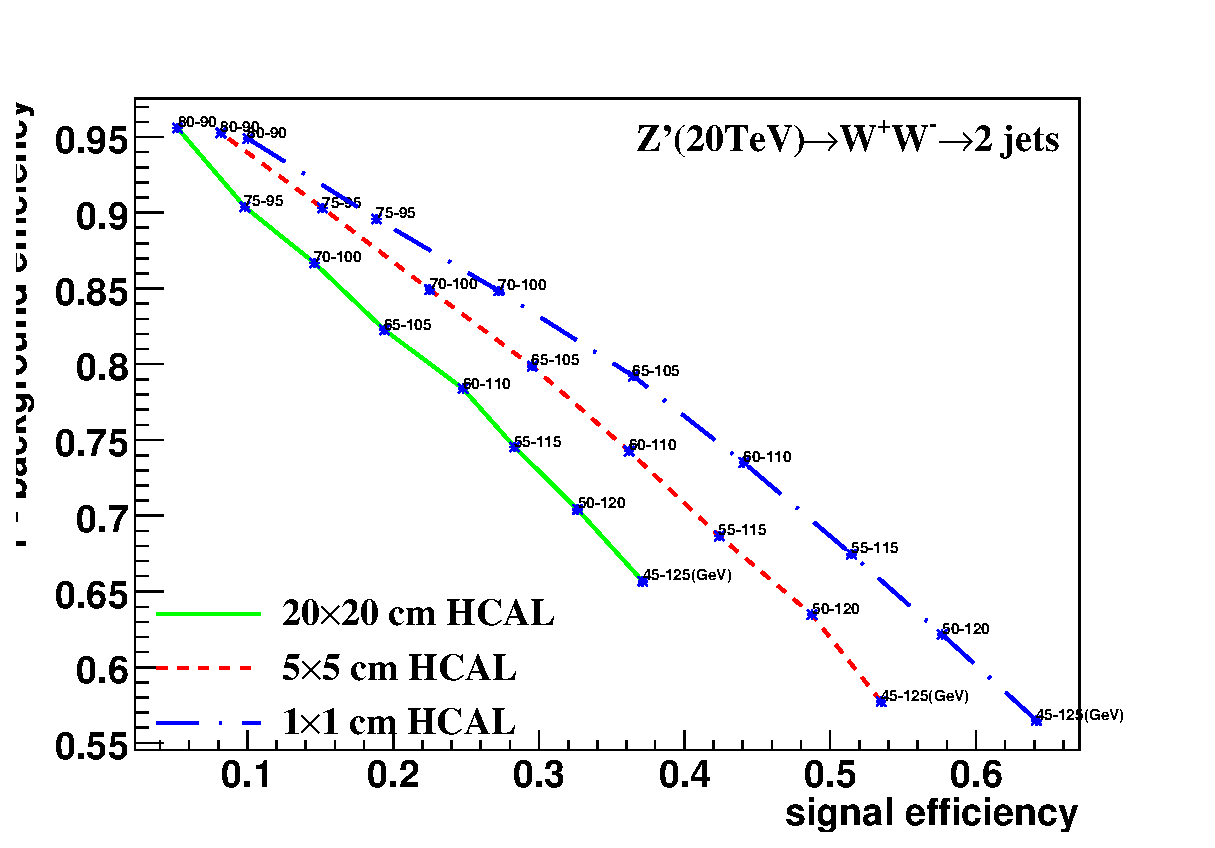
\includegraphics[width=0.43\textwidth]{figs/A_Cluster_mass_mmdt_20tev_eff_1_central_fix_at_85GeV_ww_qq.eps}
   }
   \subfigure[Central at 90TeV change width in cluster] {
   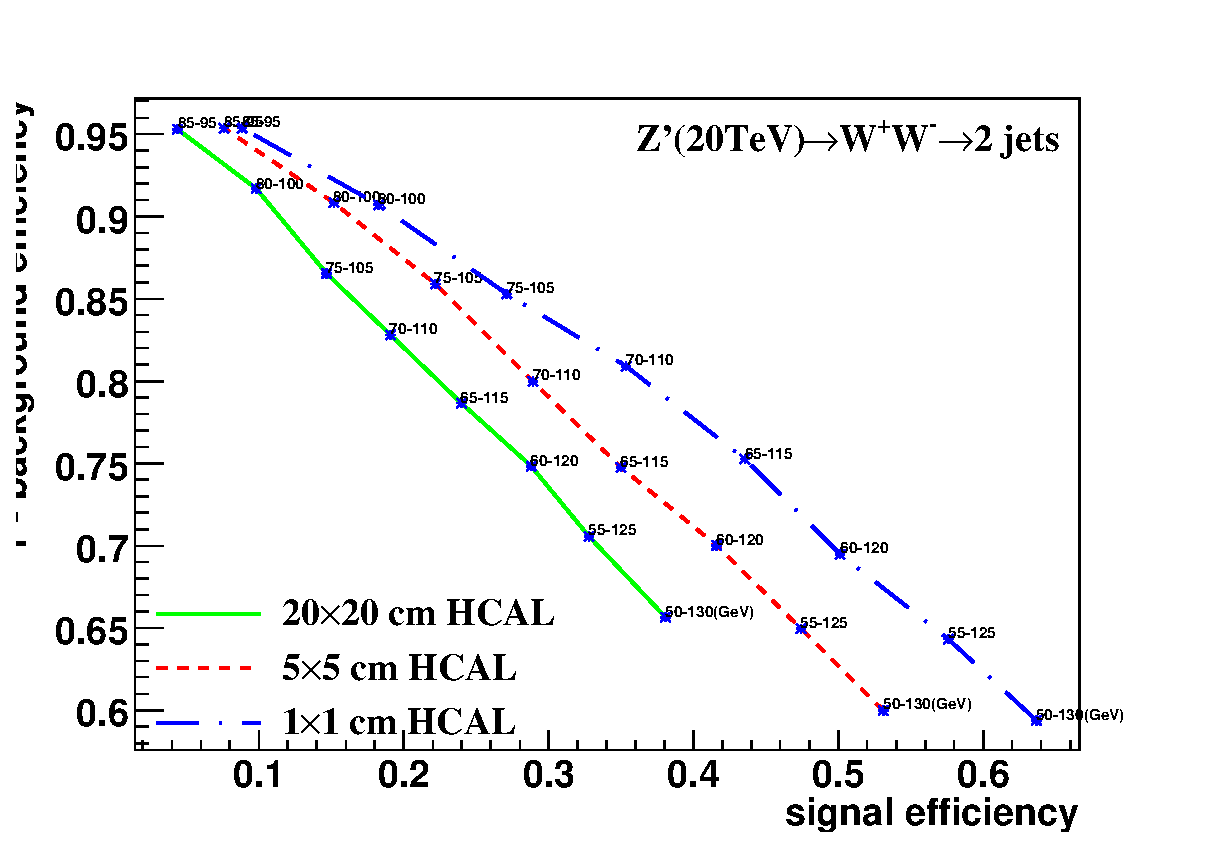
\includegraphics[width=0.43\textwidth]{figs/A_Cluster_mass_mmdt_20tev_eff_1_central_fix_at_90GeV_ww_qq.eps}
   }
   \subfigure[Central at 95TeV change width in cluster] {
   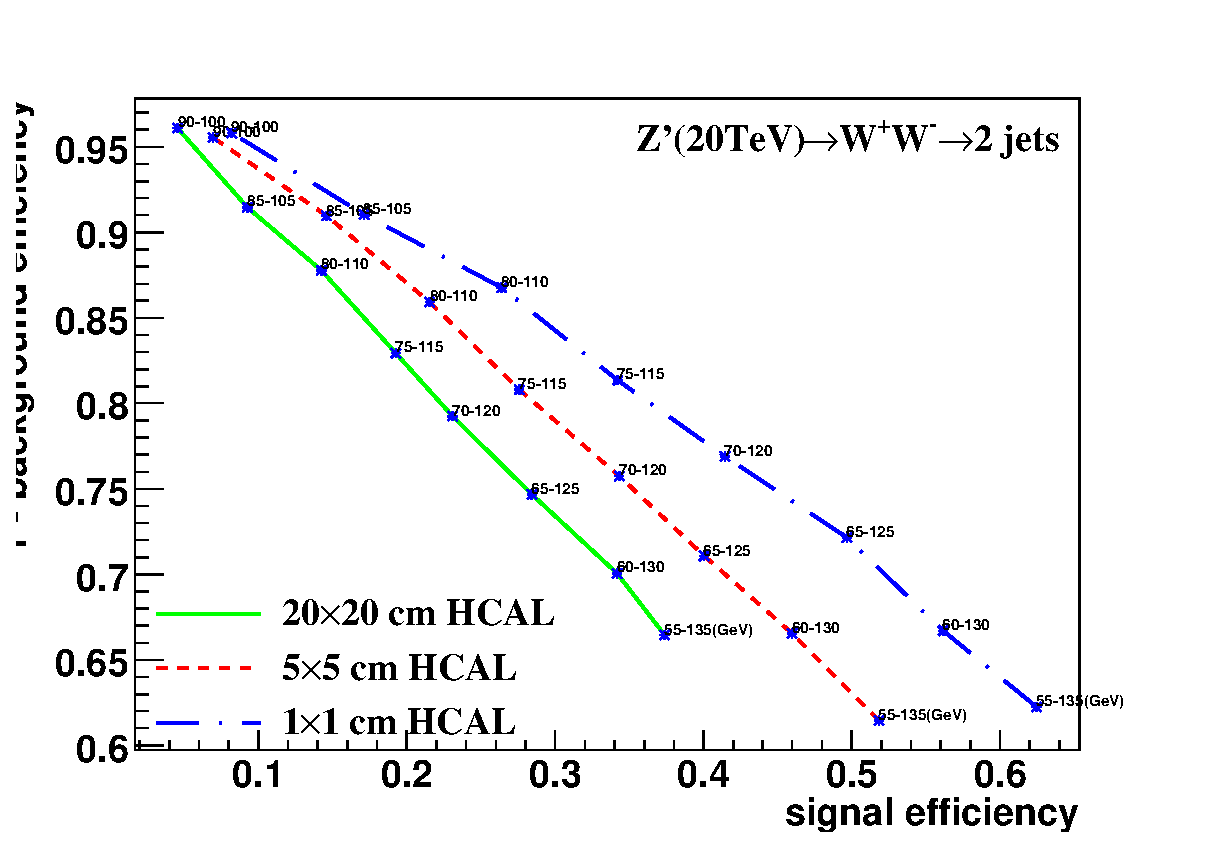
\includegraphics[width=0.43\textwidth]{figs/A_Cluster_mass_mmdt_20tev_eff_1_central_fix_at_95GeV_ww_qq.eps}
   }
   %\subfigure[Central at 100TeV change width in cluster] {
   %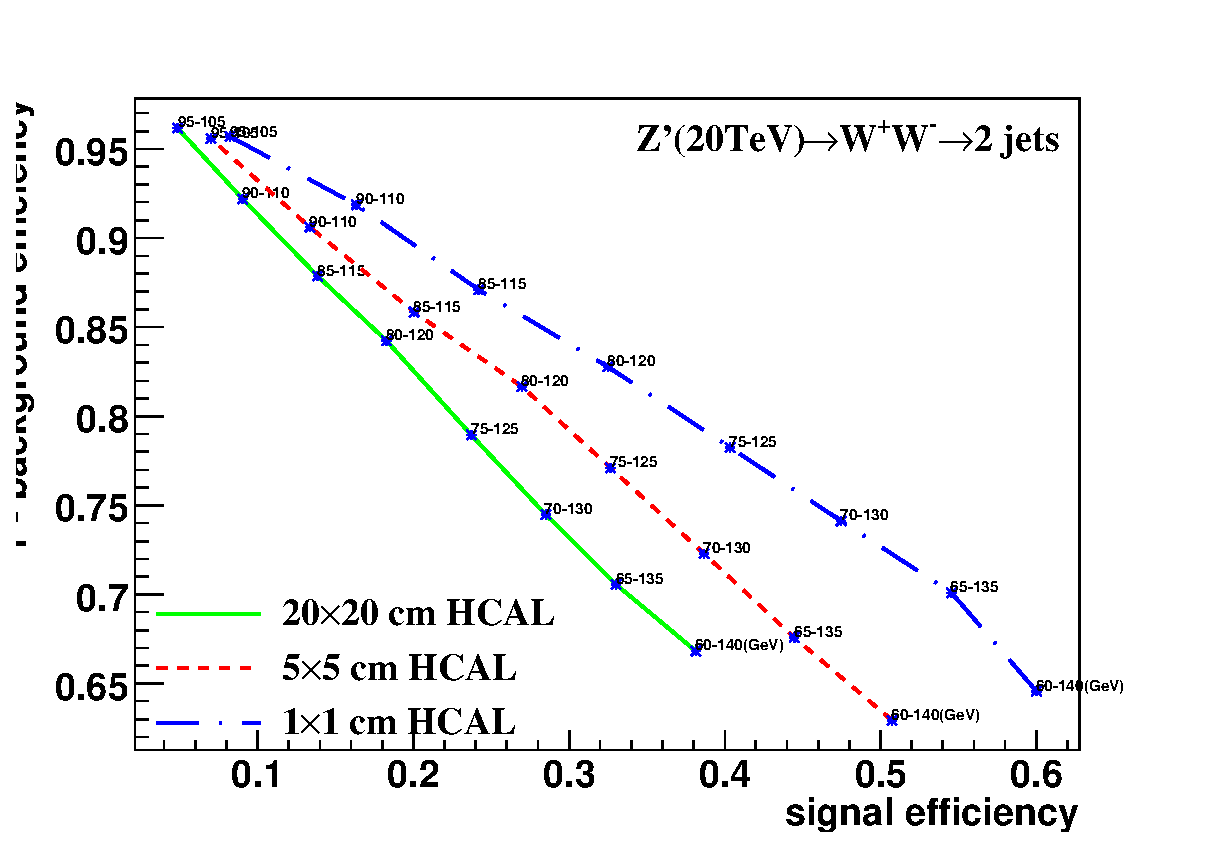
\includegraphics[width=0.43\textwidth]{figs/A_Cluster_mass_mmdt_20tev_eff_1_central_fix_at_100GeV_ww_qq.eps}
   %}
\end{center}
\caption{study of "fix central and change width" in mass soft drop at $\beta$=0, signal=ww, in 20TeV energy of collision  in different detector sizes. Cell Size in 20$\times$20, 5$\times$5, and 1$\times$1(cm$\times$cm) are shown in each picture.}
\label{fig:cluster_tau21_tau32}
\end{figure}

%50bins
\begin{figure}
\begin{center}
   \subfigure[40TeV at 20$\times$20(cm$\times$cm) in cluster] {
   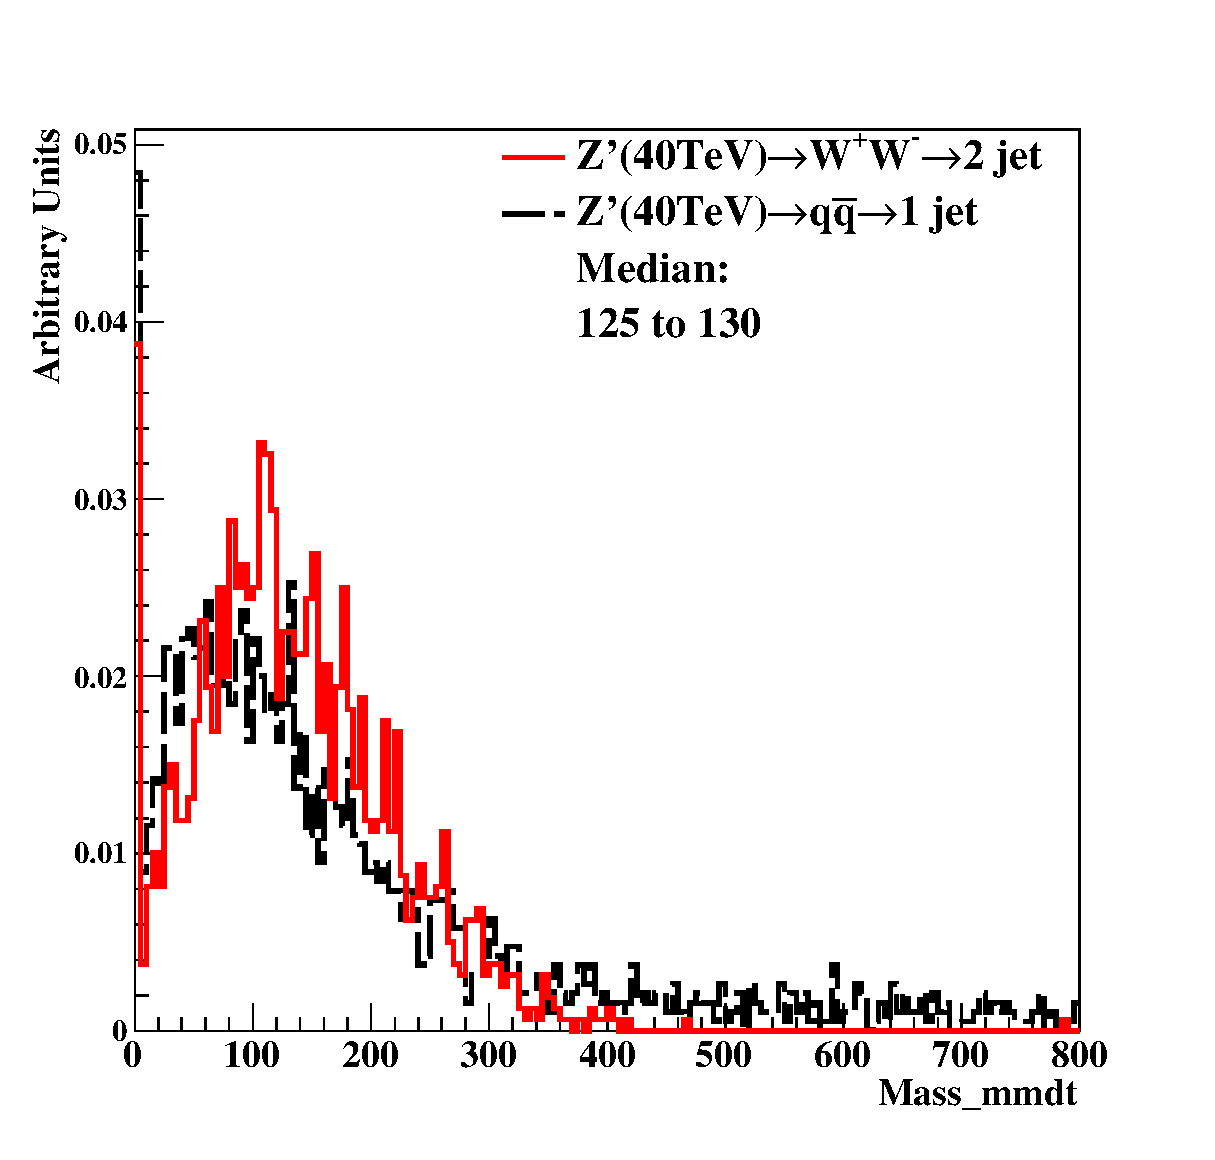
\includegraphics[width=0.43\textwidth]{figs/Dis_cluster_010_mass_mmdt_40tev_04.eps}\hfill
   }
   \subfigure[40TeV at 5$\times$5(cm$\times$cm) in cluster] {
   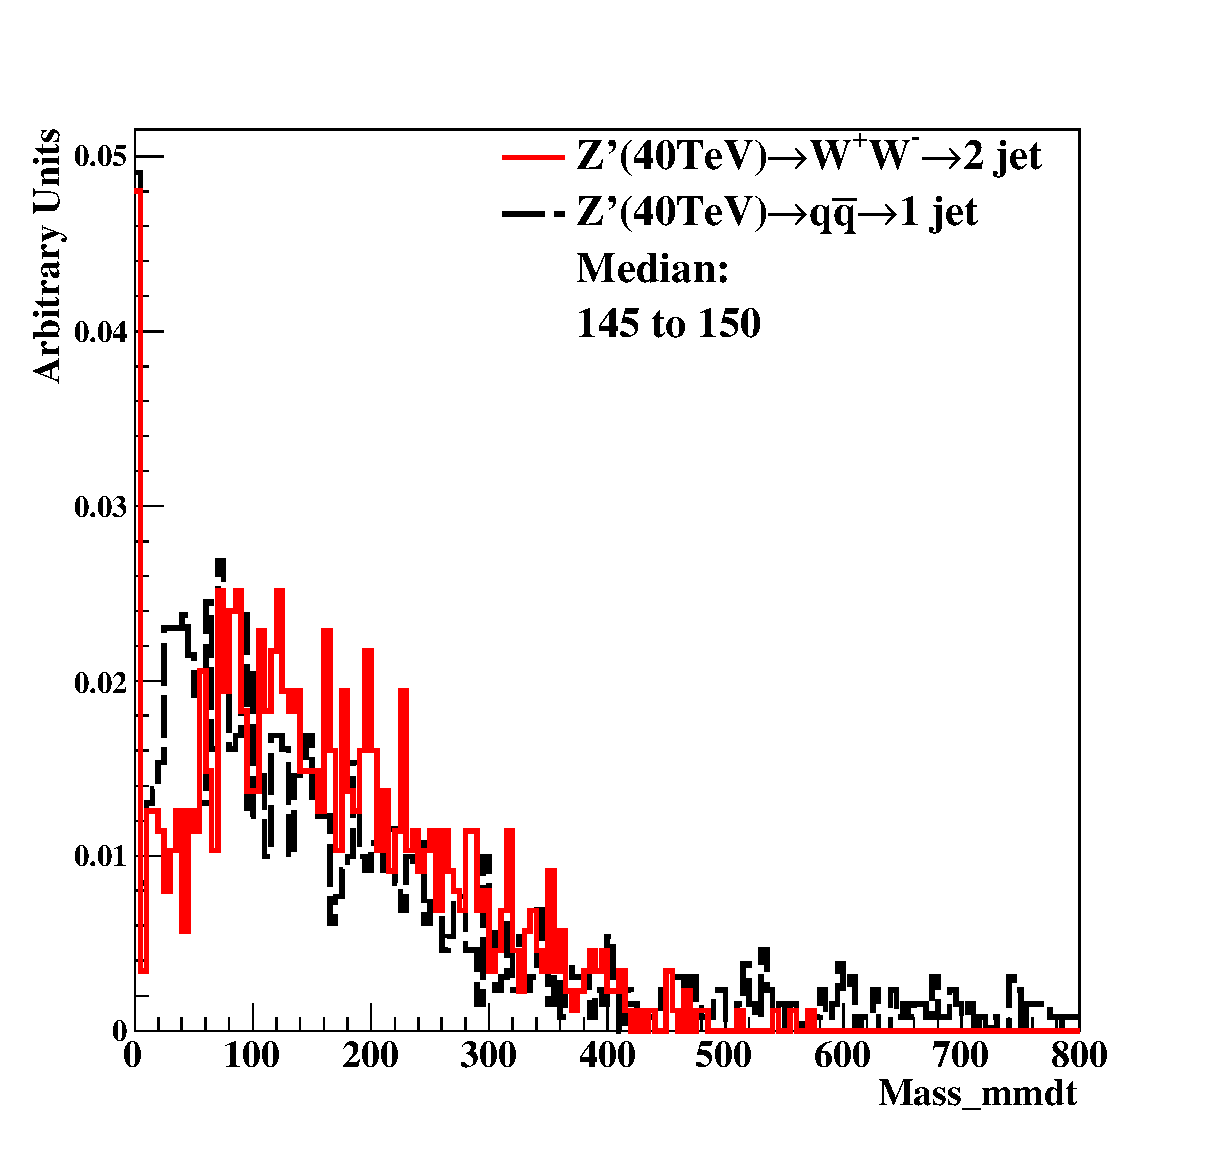
\includegraphics[width=0.43\textwidth]{figs/Dis_cluster_009_mass_mmdt_40tev_04.eps}
   }
   \subfigure[40TeV at 1$\times$1(cm$\times$cm) in cluster] {
   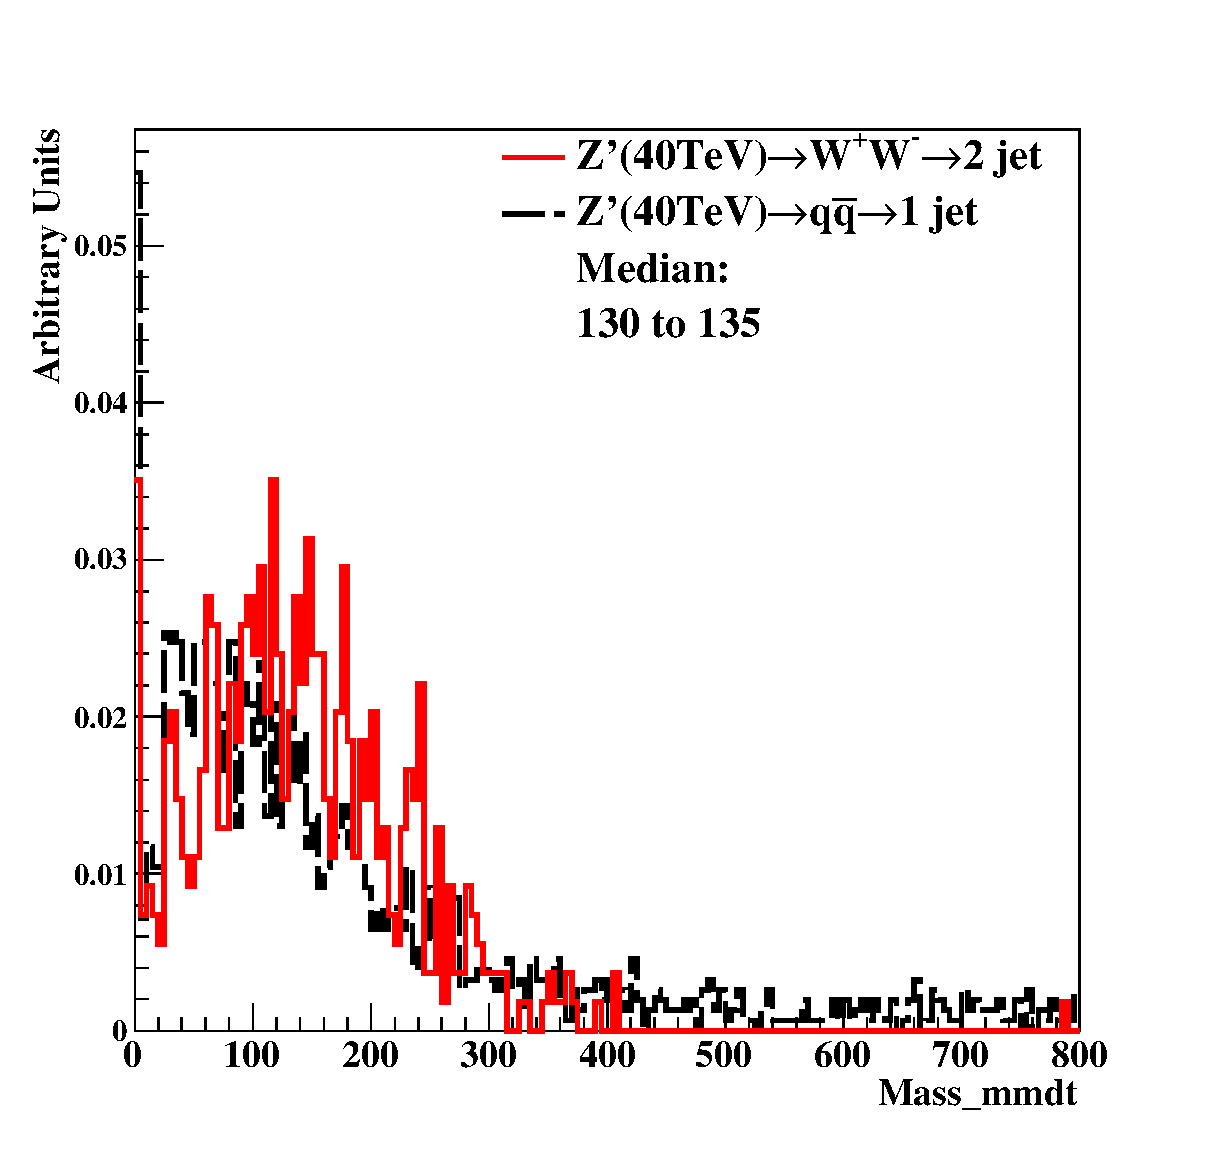
\includegraphics[width=0.43\textwidth]{figs/Dis_cluster_012_mass_mmdt_40tev_04.eps}
   }
\end{center}
\caption{Distributions of mass soft drop at $\beta$=0, signal=ww, in 40TeV energy of collision  in different detector sizes. Cell Size in 20$\times$20, 5$\times$5, and 1$\times$1(cm$\times$cm) are shown here.}
\label{fig:cluster_tau21_tau32}
\end{figure}

\begin{figure}
\begin{center}
   \subfigure[Central at 60TeV change width in cluster ] {
   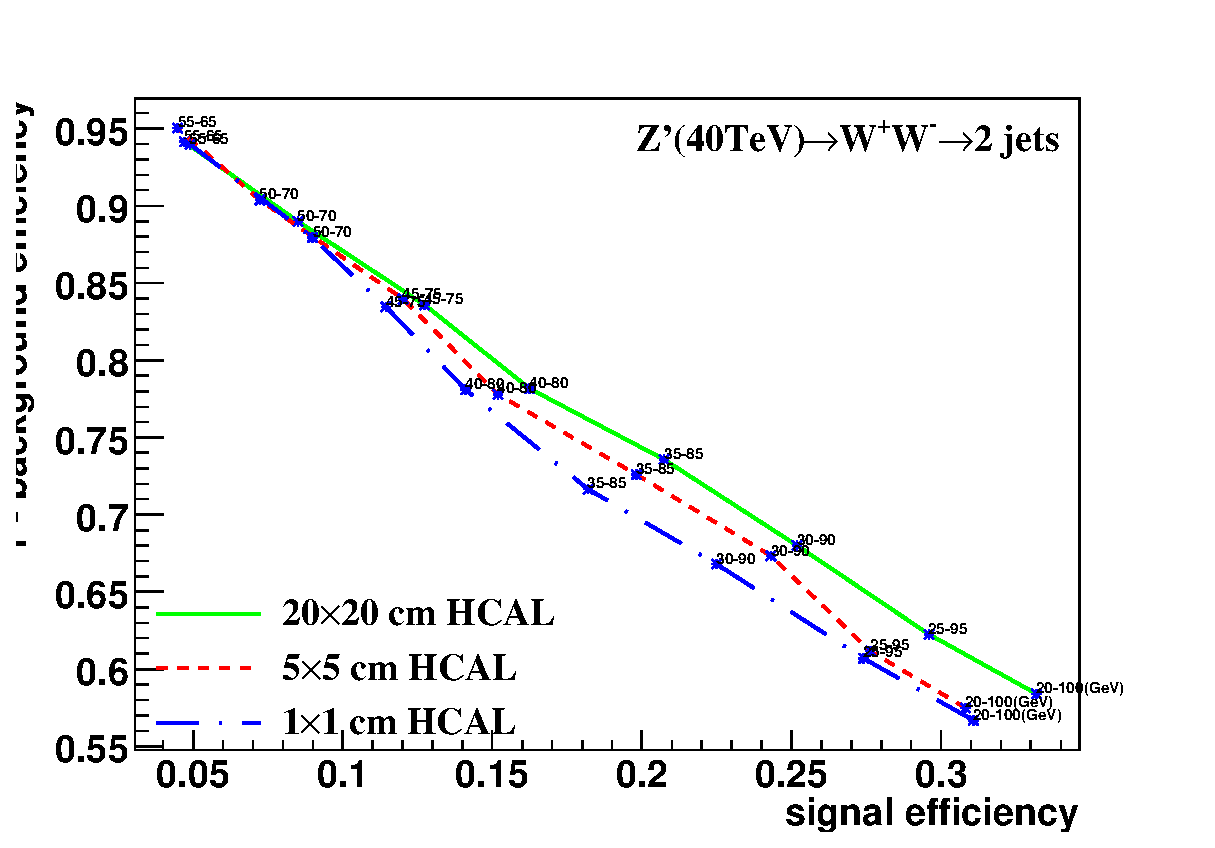
\includegraphics[width=0.43\textwidth]{figs/A_Cluster_mass_mmdt_40tev_eff_1_central_fix_at_60GeV_ww_qq.eps}\hfill
   }
   \subfigure[Central at 65TeV change width in cluster] {
   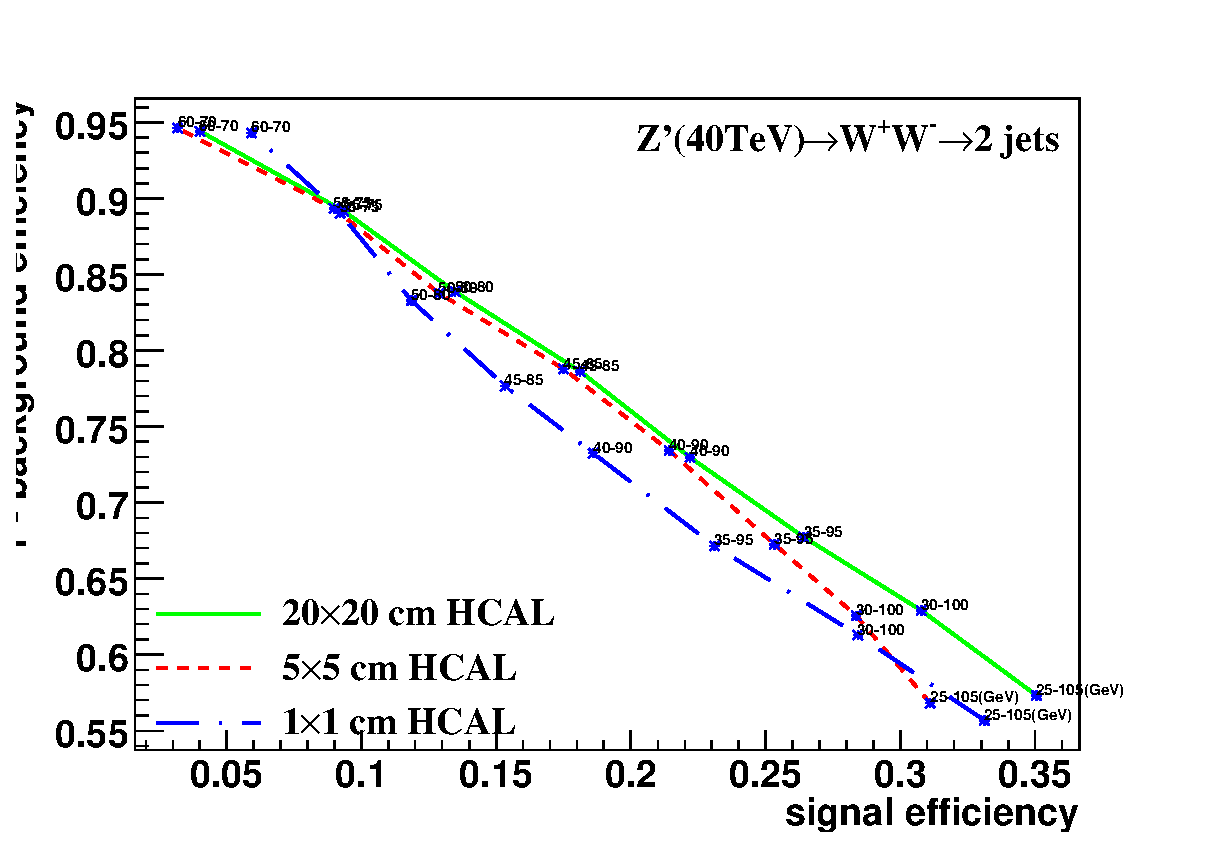
\includegraphics[width=0.43\textwidth]{figs/A_Cluster_mass_mmdt_40tev_eff_1_central_fix_at_65GeV_ww_qq.eps}
   }
   \subfigure[Central at 70TeV change width in cluster] {
   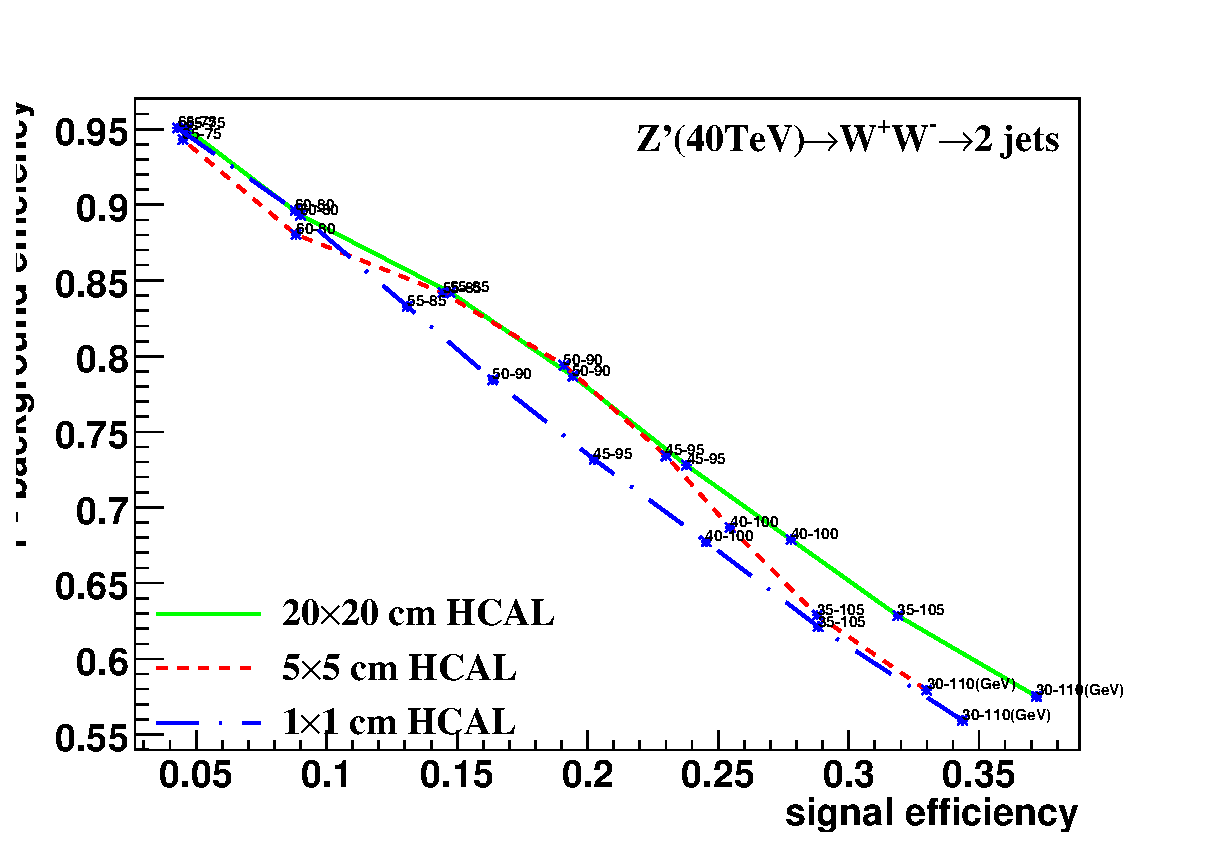
\includegraphics[width=0.43\textwidth]{figs/A_Cluster_mass_mmdt_40tev_eff_1_central_fix_at_70GeV_ww_qq.eps}
   }
   \subfigure[Central at 75TeV change width in cluster] {
   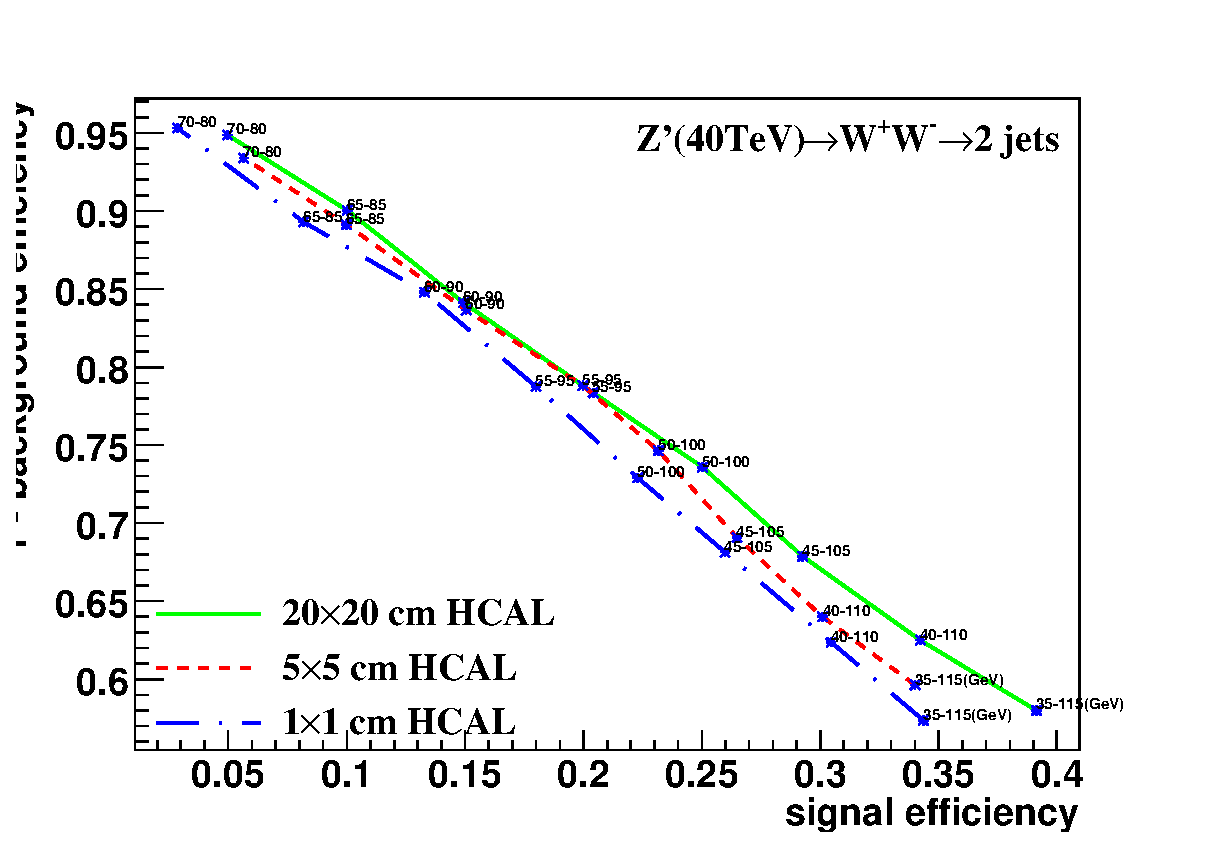
\includegraphics[width=0.43\textwidth]{figs/A_Cluster_mass_mmdt_40tev_eff_1_central_fix_at_75GeV_ww_qq.eps}
   }
   \subfigure[Central at 80TeV change width in cluster] {
   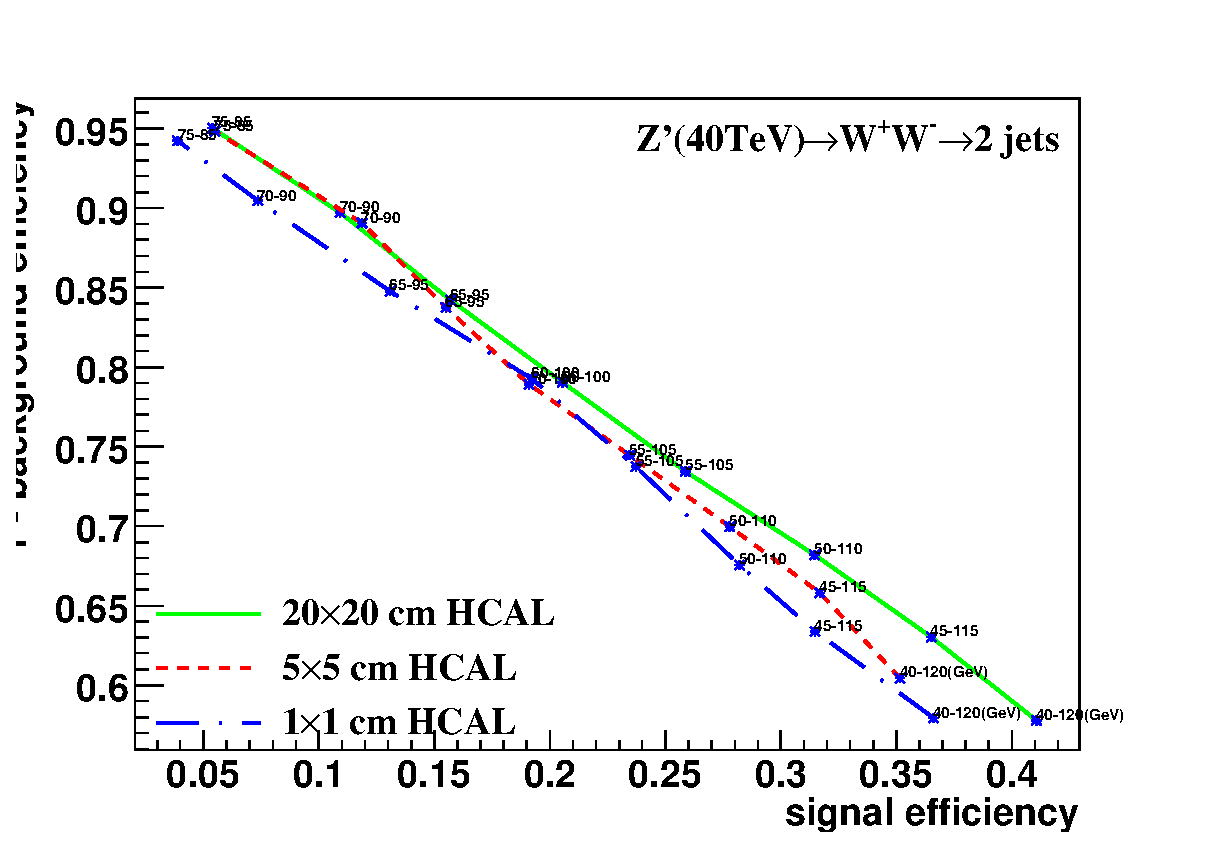
\includegraphics[width=0.43\textwidth]{figs/A_Cluster_mass_mmdt_40tev_eff_1_central_fix_at_80GeV_ww_qq.eps}
   }
   \subfigure[Central at 85TeV change width in cluster] {
   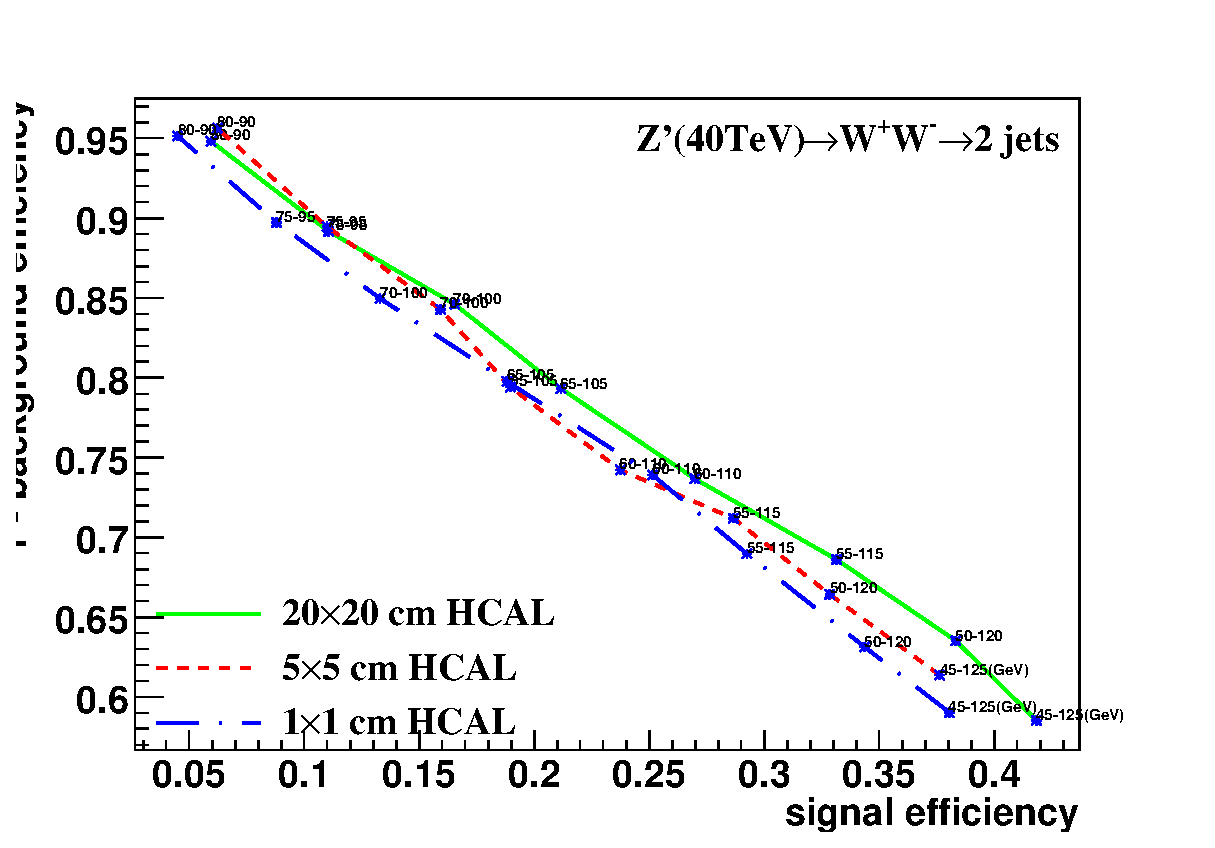
\includegraphics[width=0.43\textwidth]{figs/A_Cluster_mass_mmdt_40tev_eff_1_central_fix_at_85GeV_ww_qq.eps}
   }
   \subfigure[Central at 90TeV change width in cluster] {
   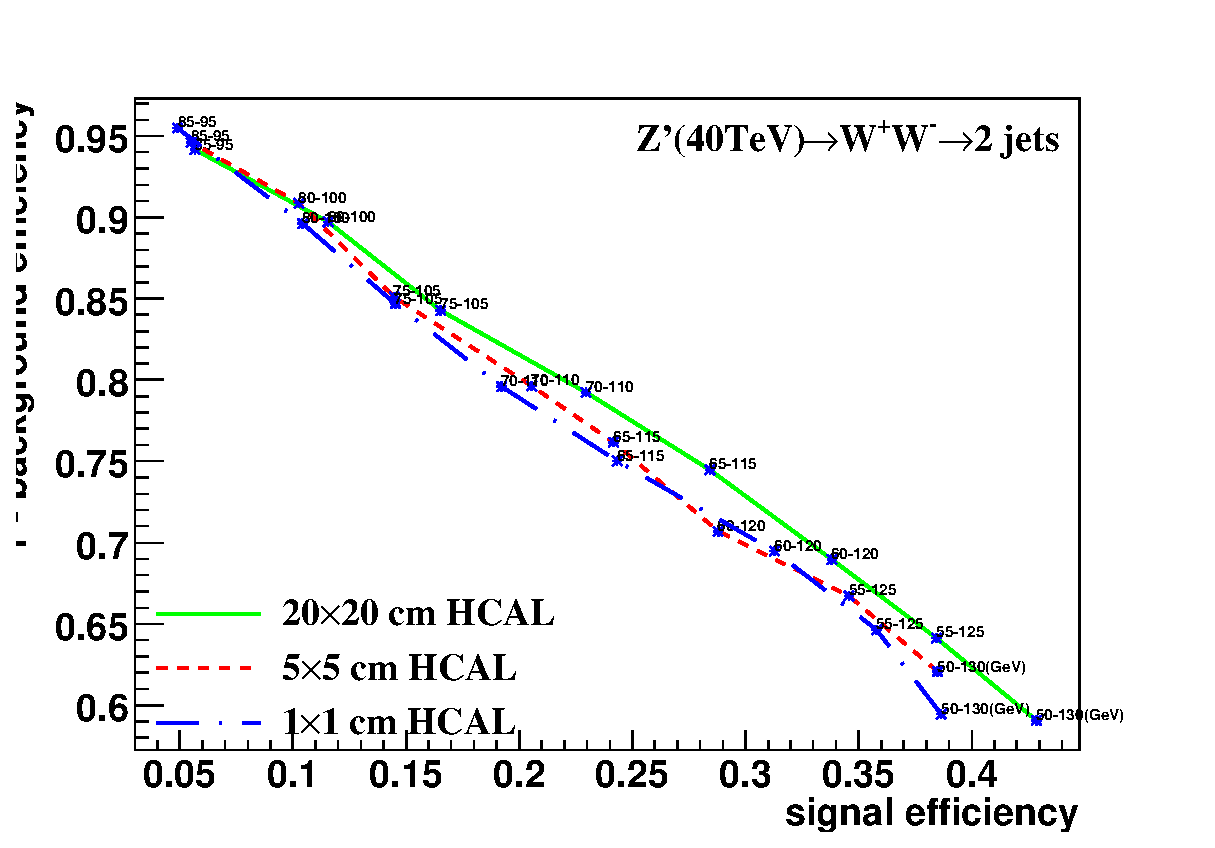
\includegraphics[width=0.43\textwidth]{figs/A_Cluster_mass_mmdt_40tev_eff_1_central_fix_at_90GeV_ww_qq.eps}
   }
   \subfigure[Central at 95TeV change width in cluster] {
   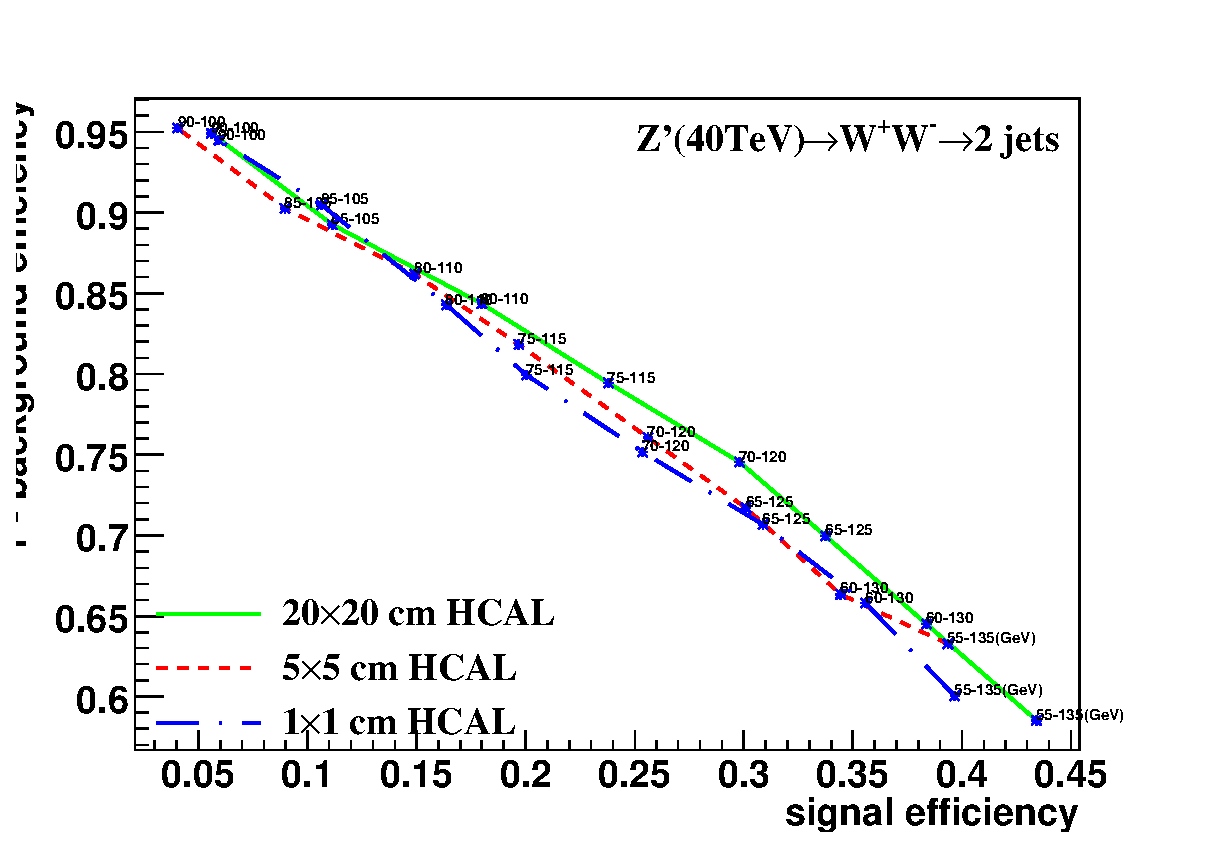
\includegraphics[width=0.43\textwidth]{figs/A_Cluster_mass_mmdt_40tev_eff_1_central_fix_at_95GeV_ww_qq.eps}
   }
   %\subfigure[Central at 100TeV change width in cluster] {
   %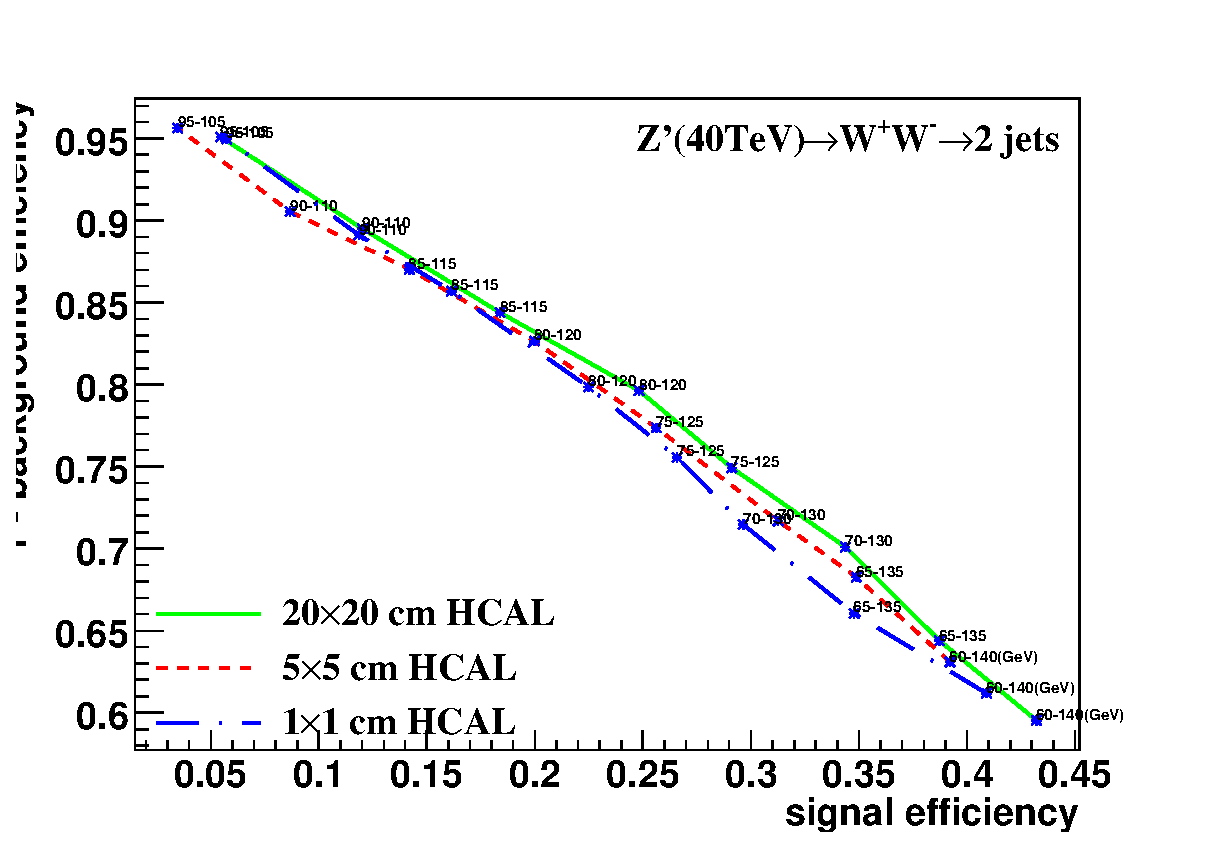
\includegraphics[width=0.43\textwidth]{figs/A_Cluster_mass_mmdt_40tev_eff_1_central_fix_at_100GeV_ww_qq.eps}
   %}
\end{center}
\caption{study of "fix central and change width" in mass soft drop at $\beta$=0, signal=ww, in 40TeV energy of collision  in different detector sizes. Cell Size in 20$\times$20, 5$\times$5, and 1$\times$1(cm$\times$cm) are shown in each picture.}
\label{fig:cluster_tau21_tau32}
\end{figure}

%50bins
\begin{figure}
\begin{center}
   \subfigure[5TeV at 20$\times$20(cm$\times$cm) in cluster] {
   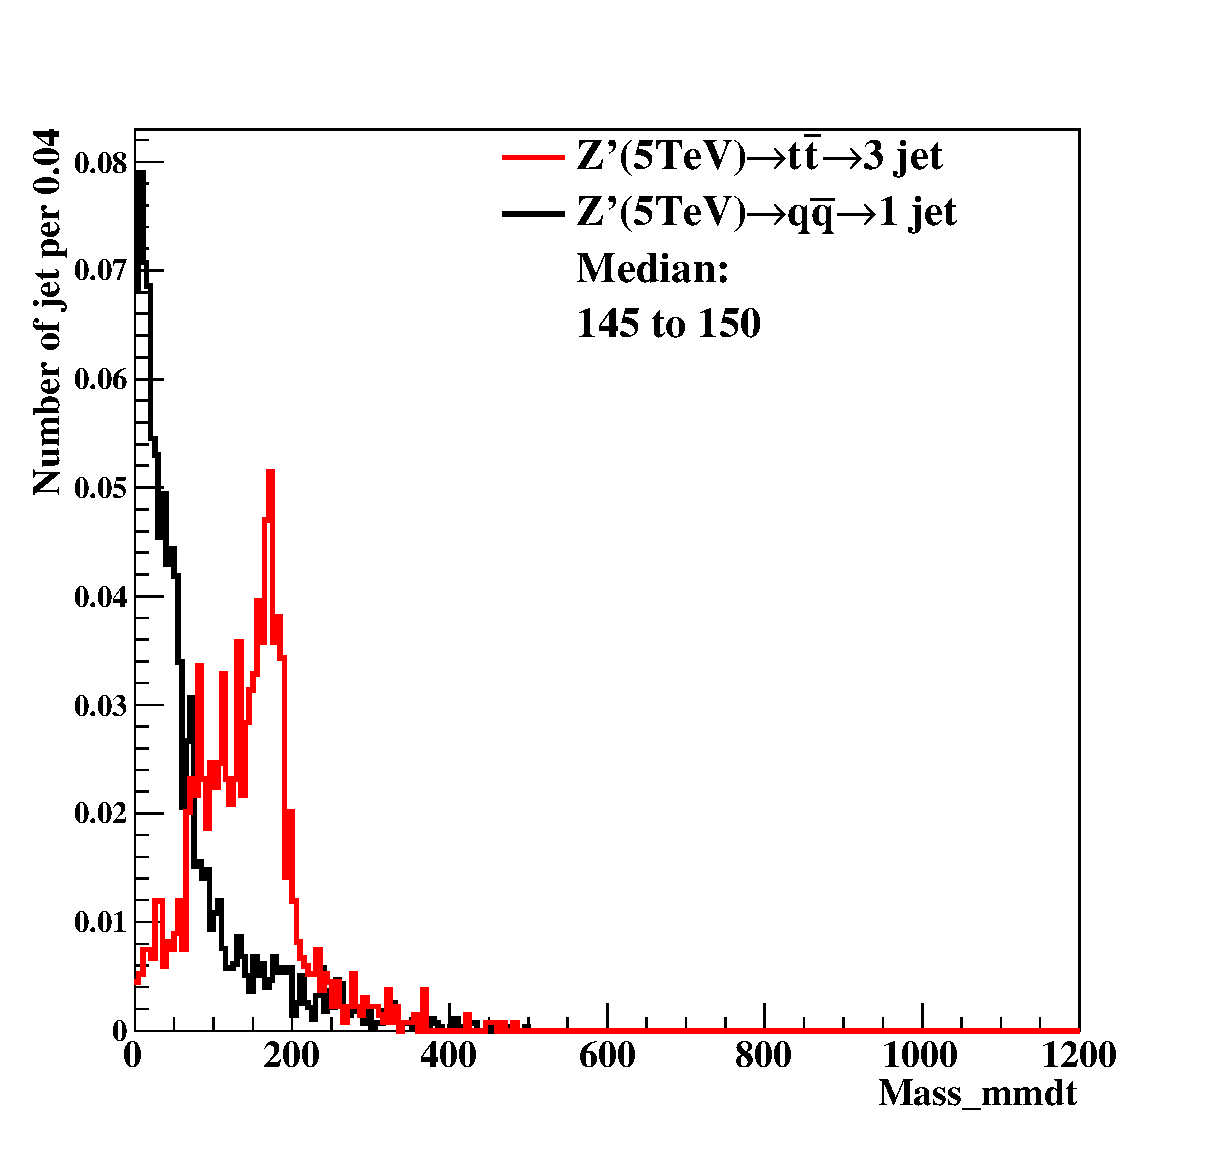
\includegraphics[width=0.43\textwidth]{figs/Dis_cluster_010_mass_mmdt_tt_5tev_04_tt.eps}\hfill
   }
   \subfigure[5TeV at 5$\times$5(cm$\times$cm) in cluster] {
   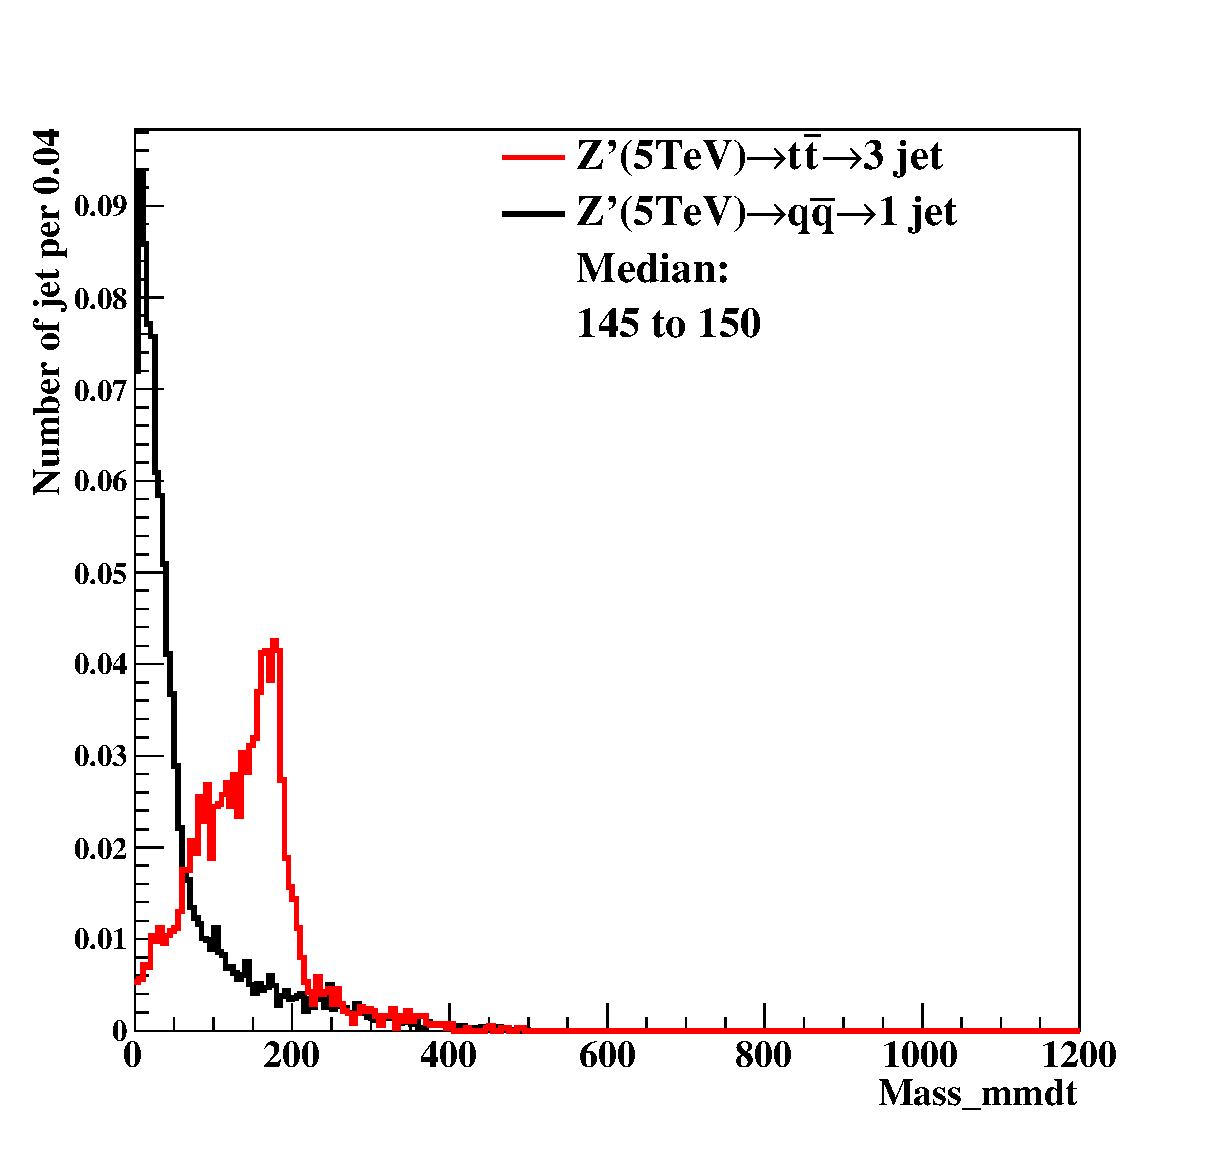
\includegraphics[width=0.43\textwidth]{figs/Dis_cluster_009_mass_mmdt_tt_5tev_04_tt.eps}
   }
   \subfigure[5TeV at 1$\times$1(cm$\times$cm) in cluster] {
   \includegraphics[width=0.43\textwidth]{figs/Dis_cluster_012_mass_mmdt_tt_5tev_04_tt.eps}
   }

\end{center}
\caption{Distributions of mass soft drop at $\beta$=0, signal=tt, in 5TeV energy of collision  in different detector sizes. Cell Size in 20$\times$20, 5$\times$5, and 1$\times$1(cm$\times$cm) are shown here.}
\label{fig:cluster_tau21_tau32}
\end{figure}

\begin{figure}
\begin{center}
   \subfigure[Central at 150TeV change width in cluster ] {
   \includegraphics[width=0.43\textwidth]{figs/A_Cluster_mass_mmdt_5tev_eff_1_central_fix_at_150GeV_tt_qq.eps}\hfill
   }
   \subfigure[Central at 155TeV change width in cluster] {
   \includegraphics[width=0.43\textwidth]{figs/A_Cluster_mass_mmdt_5tev_eff_1_central_fix_at_155GeV_tt_qq.eps}
   }
   \subfigure[Central at 160TeV change width in cluster] {
   \includegraphics[width=0.43\textwidth]{figs/A_Cluster_mass_mmdt_5tev_eff_1_central_fix_at_160GeV_tt_qq.eps}
   }
   \subfigure[Central at 165TeV change width in cluster] {
   \includegraphics[width=0.43\textwidth]{figs/A_Cluster_mass_mmdt_5tev_eff_1_central_fix_at_165GeV_tt_qq.eps}
   }
   \subfigure[Central at 170TeV change width in cluster] {
   \includegraphics[width=0.43\textwidth]{figs/A_Cluster_mass_mmdt_5tev_eff_1_central_fix_at_170GeV_tt_qq.eps}
   }
   \subfigure[Central at 175TeV change width in cluster] {
   \includegraphics[width=0.43\textwidth]{figs/A_Cluster_mass_mmdt_5tev_eff_1_central_fix_at_175GeV_tt_qq.eps}
   }
   \subfigure[Central at 180TeV change width in cluster] {
   \includegraphics[width=0.43\textwidth]{figs/A_Cluster_mass_mmdt_5tev_eff_1_central_fix_at_180GeV_tt_qq.eps}
   }
   \subfigure[Central at 185TeV change width in cluster] {
   \includegraphics[width=0.43\textwidth]{figs/A_Cluster_mass_mmdt_5tev_eff_1_central_fix_at_185GeV_tt_qq.eps}
   }
   %\subfigure[Central at 190TeV change width in cluster] {
   %\includegraphics[width=0.43\textwidth]{figs/A_Cluster_mass_mmdt_5tev_eff_1_central_fix_at_190GeV_tt_qq.eps}
   %}


\end{center}
\caption{study of "fix central and change width" in mass soft drop at $\beta$=0, signal=tt, in 5TeV energy of collision  in different detector sizes. Cell Size in 20$\times$20, 5$\times$5, and 1$\times$1(cm$\times$cm) are shown in each picture.}
\label{fig:cluster_tau21_tau32}
\end{figure}

%50bins
\begin{figure}
\begin{center}
   \subfigure[10TeV at 20$\times$20(cm$\times$cm) in cluster] {
   \includegraphics[width=0.43\textwidth]{figs/Dis_cluster_010_mass_mmdt_tt_10tev_04_tt.eps}\hfill
   }
   \subfigure[10TeV at 5$\times$5(cm$\times$cm) in cluster] {
   \includegraphics[width=0.43\textwidth]{figs/Dis_cluster_009_mass_mmdt_tt_10tev_04_tt.eps}
   }
   \subfigure[10TeV at 1$\times$1(cm$\times$cm) in cluster] {
   \includegraphics[width=0.43\textwidth]{figs/Dis_cluster_012_mass_mmdt_tt_10tev_04_tt.eps}
   }

\end{center}
\caption{Distributions of mass soft drop at $\beta$=0, signal=tt, in 10TeV energy of collision  in different detector sizes. Cell Size in 20$\times$20, 5$\times$5, and 1$\times$1(cm$\times$cm) are shown here.}
\label{fig:cluster_tau21_tau32}
\end{figure}

\begin{figure}
\begin{center}
   \subfigure[Central at 150TeV change width in cluster ] {
   \includegraphics[width=0.43\textwidth]{figs/A_Cluster_mass_mmdt_10tev_eff_1_central_fix_at_150GeV_tt_qq.eps}\hfill
   }
   \subfigure[Central at 155TeV change width in cluster] {
   \includegraphics[width=0.43\textwidth]{figs/A_Cluster_mass_mmdt_10tev_eff_1_central_fix_at_155GeV_tt_qq.eps}
   }
   \subfigure[Central at 160TeV change width in cluster] {
   \includegraphics[width=0.43\textwidth]{figs/A_Cluster_mass_mmdt_10tev_eff_1_central_fix_at_160GeV_tt_qq.eps}
   }
   \subfigure[Central at 165TeV change width in cluster] {
   \includegraphics[width=0.43\textwidth]{figs/A_Cluster_mass_mmdt_10tev_eff_1_central_fix_at_165GeV_tt_qq.eps}
   }
   \subfigure[Central at 170TeV change width in cluster] {
   \includegraphics[width=0.43\textwidth]{figs/A_Cluster_mass_mmdt_10tev_eff_1_central_fix_at_170GeV_tt_qq.eps}
   }
   \subfigure[Central at 175TeV change width in cluster] {
   \includegraphics[width=0.43\textwidth]{figs/A_Cluster_mass_mmdt_10tev_eff_1_central_fix_at_175GeV_tt_qq.eps}
   }
   \subfigure[Central at 180TeV change width in cluster] {
   \includegraphics[width=0.43\textwidth]{figs/A_Cluster_mass_mmdt_10tev_eff_1_central_fix_at_180GeV_tt_qq.eps}
   }
   \subfigure[Central at 185TeV change width in cluster] {
   \includegraphics[width=0.43\textwidth]{figs/A_Cluster_mass_mmdt_10tev_eff_1_central_fix_at_185GeV_tt_qq.eps}
   }
   %\subfigure[Central at 190TeV change width in cluster] {
   %\includegraphics[width=0.43\textwidth]{figs/A_Cluster_mass_mmdt_10tev_eff_1_central_fix_at_190GeV_tt_qq.eps}
   %}


\end{center}
\caption{study of "fix central and change width" in mass soft drop at $\beta$=0, signal=tt, in 10TeV energy of collision  in different detector sizes. Cell Size in 20$\times$20, 5$\times$5, and 1$\times$1(cm$\times$cm) are shown in each picture.}
\label{fig:cluster_tau21_tau32}
\end{figure}

%50bins
\begin{figure}
\begin{center}
   \subfigure[20TeV at 20$\times$20(cm$\times$cm) in cluster] {
   \includegraphics[width=0.43\textwidth]{figs/Dis_cluster_010_mass_mmdt_tt_20tev_04_tt.eps}\hfill
   }
   \subfigure[20TeV at 5$\times$5(cm$\times$cm) in cluster] {
   \includegraphics[width=0.43\textwidth]{figs/Dis_cluster_009_mass_mmdt_tt_20tev_04_tt.eps}
   }
   \subfigure[20TeV at 1$\times$1(cm$\times$cm) in cluster] {
   \includegraphics[width=0.43\textwidth]{figs/Dis_cluster_012_mass_mmdt_tt_20tev_04_tt.eps}
   }

\end{center}
\caption{Distributions of mass soft drop at $\beta$=0, signal=tt, in 20TeV energy of collision  in different detector sizes. Cell Size in 20$\times$20, 5$\times$5, and 1$\times$1(cm$\times$cm) are shown here.}
\label{fig:cluster_tau21_tau32}
\end{figure}

\begin{figure}
\begin{center}
   \subfigure[Central at 150TeV change width in cluster ] {
   \includegraphics[width=0.43\textwidth]{figs/A_Cluster_mass_mmdt_20tev_eff_1_central_fix_at_150GeV_tt_qq.eps}\hfill
   }
   \subfigure[Central at 155TeV change width in cluster] {
   \includegraphics[width=0.43\textwidth]{figs/A_Cluster_mass_mmdt_20tev_eff_1_central_fix_at_155GeV_tt_qq.eps}
   }
   \subfigure[Central at 160TeV change width in cluster] {
   \includegraphics[width=0.43\textwidth]{figs/A_Cluster_mass_mmdt_20tev_eff_1_central_fix_at_160GeV_tt_qq.eps}
   }
   \subfigure[Central at 165TeV change width in cluster] {
   \includegraphics[width=0.43\textwidth]{figs/A_Cluster_mass_mmdt_20tev_eff_1_central_fix_at_165GeV_tt_qq.eps}
   }
   \subfigure[Central at 170TeV change width in cluster] {
   \includegraphics[width=0.43\textwidth]{figs/A_Cluster_mass_mmdt_20tev_eff_1_central_fix_at_170GeV_tt_qq.eps}
   }
   \subfigure[Central at 175TeV change width in cluster] {
   \includegraphics[width=0.43\textwidth]{figs/A_Cluster_mass_mmdt_20tev_eff_1_central_fix_at_175GeV_tt_qq.eps}
   }
   \subfigure[Central at 180TeV change width in cluster] {
   \includegraphics[width=0.43\textwidth]{figs/A_Cluster_mass_mmdt_20tev_eff_1_central_fix_at_180GeV_tt_qq.eps}
   }
   \subfigure[Central at 185TeV change width in cluster] {
   \includegraphics[width=0.43\textwidth]{figs/A_Cluster_mass_mmdt_20tev_eff_1_central_fix_at_185GeV_tt_qq.eps}
   }
   %\subfigure[Central at 190TeV change width in cluster] {
   %\includegraphics[width=0.43\textwidth]{figs/A_Cluster_mass_mmdt_20tev_eff_1_central_fix_at_190GeV_tt_qq.eps}
   %}
\end{center}
\caption{study of "fix central and change width" in mass soft drop at $\beta$=0, signal=tt, in 20TeV energy of collision  in different detector sizes. Cell Size in 20$\times$20, 5$\times$5, and 1$\times$1(cm$\times$cm) are shown in each picture.}
\label{fig:cluster_tau21_tau32}
\end{figure}

%50bins
\begin{figure}
\begin{center}
   \subfigure[40TeV at 20$\times$20(cm$\times$cm) in cluster] {
   \includegraphics[width=0.43\textwidth]{figs/Dis_cluster_010_mass_mmdt_tt_40tev_04_tt.eps}\hfill
   }
   \subfigure[40TeV at 5$\times$5(cm$\times$cm) in cluster] {
   \includegraphics[width=0.43\textwidth]{figs/Dis_cluster_009_mass_mmdt_tt_40tev_04_tt.eps}
   }
   \subfigure[40TeV at 1$\times$1(cm$\times$cm) in cluster] {
   \includegraphics[width=0.43\textwidth]{figs/Dis_cluster_012_mass_mmdt_tt_40tev_04_tt.eps}
   }

\end{center}
\caption{Distributions of mass soft drop at $\beta$=0, signal=tt, in 40TeV energy of collision  in different detector sizes. Cell Size in 20$\times$20, 5$\times$5, and 1$\times$1(cm$\times$cm) are shown here.}
\label{fig:cluster_tau21_tau32}
\end{figure}

\begin{figure}
\begin{center}
   \subfigure[Central at 150TeV change width in cluster ] {
   \includegraphics[width=0.43\textwidth]{figs/A_Cluster_mass_mmdt_40tev_eff_1_central_fix_at_150GeV_tt_qq.eps}\hfill
   }
   \subfigure[Central at 155TeV change width in cluster] {
   \includegraphics[width=0.43\textwidth]{figs/A_Cluster_mass_mmdt_40tev_eff_1_central_fix_at_155GeV_tt_qq.eps}
   }
   \subfigure[Central at 160TeV change width in cluster] {
   \includegraphics[width=0.43\textwidth]{figs/A_Cluster_mass_mmdt_40tev_eff_1_central_fix_at_160GeV_tt_qq.eps}
   }
   \subfigure[Central at 165TeV change width in cluster] {
   \includegraphics[width=0.43\textwidth]{figs/A_Cluster_mass_mmdt_40tev_eff_1_central_fix_at_165GeV_tt_qq.eps}
   }
   \subfigure[Central at 170TeV change width in cluster] {
   \includegraphics[width=0.43\textwidth]{figs/A_Cluster_mass_mmdt_40tev_eff_1_central_fix_at_170GeV_tt_qq.eps}
   }
   \subfigure[Central at 175TeV change width in cluster] {
   \includegraphics[width=0.43\textwidth]{figs/A_Cluster_mass_mmdt_40tev_eff_1_central_fix_at_175GeV_tt_qq.eps}
   }
   \subfigure[Central at 180TeV change width in cluster] {
   \includegraphics[width=0.43\textwidth]{figs/A_Cluster_mass_mmdt_40tev_eff_1_central_fix_at_180GeV_tt_qq.eps}
   }
   \subfigure[Central at 185TeV change width in cluster] {
   \includegraphics[width=0.43\textwidth]{figs/A_Cluster_mass_mmdt_40tev_eff_1_central_fix_at_185GeV_tt_qq.eps}
   }
\end{center}
\caption{study of "fix central and change width" in mass soft drop at $\beta$=0, signal=tt, in 40TeV energy of collision  in different detector sizes. Cell Size in 20$\times$20, 5$\times$5, and 1$\times$1(cm$\times$cm) are shown in each picture.}
\label{fig:cluster_tau21}
\end{figure}

%50bins
\begin{figure}
\begin{center}
   \subfigure[5TeV at 20$\times$20(cm$\times$cm) in cluster] {
   \includegraphics[width=0.43\textwidth]{figs/Dis_cluster_010_mass_sdb2_ww_5tev_04.eps}\hfill
   }
   \subfigure[5TeV at 5$\times$5(cm$\times$cm) in cluster] {
   \includegraphics[width=0.43\textwidth]{figs/Dis_cluster_009_mass_sdb2_ww_5tev_04.eps}
   }
   \subfigure[5TeV at 1$\times$1(cm$\times$cm) in cluster] {
   \includegraphics[width=0.43\textwidth]{figs/Dis_cluster_012_mass_sdb2_ww_5tev_04.eps}
   }
\end{center}
\caption{Distributions of mass soft drop at $\beta$=2, signal=ww, in 5TeV energy of collision  in different detector sizes. Cell Size in 20$\times$20, 5$\times$5, and 1$\times$1(cm$\times$cm) are shown here.}
\label{fig:cluster_tau21_tau32}
\end{figure}


\section{Studies of signal and background separation using Mass soft drop at $\beta=2$ using fix central and change width method}
\begin{figure}
\begin{center}
   \subfigure[Central at 80TeV change width in cluster ] {
   \includegraphics[width=0.43\textwidth]{figs/A_Cluster_mass_sdb2_5tev_eff_1_central_fix_at_80GeV_ww_qq.eps}\hfill
   }
   \subfigure[Central at 85TeV change width in cluster] {
   \includegraphics[width=0.43\textwidth]{figs/A_Cluster_mass_sdb2_5tev_eff_1_central_fix_at_85GeV_ww_qq.eps}
   }
   \subfigure[Central at 90TeV change width in cluster] {
   \includegraphics[width=0.43\textwidth]{figs/A_Cluster_mass_sdb2_5tev_eff_1_central_fix_at_90GeV_ww_qq.eps}
   }
   \subfigure[Central at 95TeV change width in cluster] {
   \includegraphics[width=0.43\textwidth]{figs/A_Cluster_mass_sdb2_5tev_eff_1_central_fix_at_95GeV_ww_qq.eps}
   }
   \subfigure[Central at 100TeV change width in cluster] {
   \includegraphics[width=0.43\textwidth]{figs/A_Cluster_mass_sdb2_5tev_eff_1_central_fix_at_100GeV_ww_qq.eps}
   }
   \subfigure[Central at 105TeV change width in cluster] {
   \includegraphics[width=0.43\textwidth]{figs/A_Cluster_mass_sdb2_5tev_eff_1_central_fix_at_105GeV_ww_qq.eps}
   }
   \subfigure[Central at 110TeV change width in cluster] {
   \includegraphics[width=0.43\textwidth]{figs/A_Cluster_mass_sdb2_5tev_eff_1_central_fix_at_110GeV_ww_qq.eps}
   }
   \subfigure[Central at 115TeV change width in cluster] {
   \includegraphics[width=0.43\textwidth]{figs/A_Cluster_mass_sdb2_5tev_eff_1_central_fix_at_115GeV_ww_qq.eps}
   }
   %\subfigure[Central at 120TeV change width in cluster] {
   %\includegraphics[width=0.43\textwidth]{figs/A_Cluster_mass_sdb2_5tev_eff_1_central_fix_at_120GeV_ww_qq.eps}
   %}
\end{center}
\caption{study of "fix central and change width" in mass soft drop at $\beta$=2, signal=ww, in 5TeV energy of collision  in different detector sizes. Cell Size in 20$\times$20, 5$\times$5, and 1$\times$1(cm$\times$cm) are shown in each picture.}
\label{fig:cluster_tau21_tau32}
\end{figure}

%50bins
\begin{figure}
\begin{center}
   \subfigure[10TeV at 20$\times$20(cm$\times$cm) in cluster] {
   \includegraphics[width=0.43\textwidth]{figs/Dis_cluster_010_mass_sdb2_ww_10tev_04.eps}\hfill
   }
   \subfigure[10TeV at 5$\times$5(cm$\times$cm) in cluster] {
   \includegraphics[width=0.43\textwidth]{figs/Dis_cluster_009_mass_sdb2_ww_10tev_04.eps}
   }
   \subfigure[10TeV at 1$\times$1(cm$\times$cm) in cluster] {
   \includegraphics[width=0.43\textwidth]{figs/Dis_cluster_012_mass_sdb2_ww_10tev_04.eps}
   }

\end{center}
\caption{Distributions of mass soft drop at $\beta$=2, signal=ww, in 10TeV energy of collision  in different detector sizes. Cell Size in 20$\times$20, 5$\times$5, and 1$\times$1(cm$\times$cm) are shown here.}
\label{fig:cluster_tau21_tau32}
\end{figure}

\begin{figure}
\begin{center}
   \subfigure[Central at 105TeV change width in cluster ] {
   \includegraphics[width=0.43\textwidth]{figs/A_Cluster_mass_sdb2_10tev_eff_1_central_fix_at_105GeV_ww_qq.eps}\hfill
   }
   \subfigure[Central at 110TeV change width in cluster] {
   \includegraphics[width=0.43\textwidth]{figs/A_Cluster_mass_sdb2_10tev_eff_1_central_fix_at_110GeV_ww_qq.eps}
   }
   \subfigure[Central at 115TeV change width in cluster] {
   \includegraphics[width=0.43\textwidth]{figs/A_Cluster_mass_sdb2_10tev_eff_1_central_fix_at_115GeV_ww_qq.eps}
   }
   \subfigure[Central at 120TeV change width in cluster] {
   \includegraphics[width=0.43\textwidth]{figs/A_Cluster_mass_sdb2_10tev_eff_1_central_fix_at_120GeV_ww_qq.eps}
   }
   \subfigure[Central at 125TeV change width in cluster] {
   \includegraphics[width=0.43\textwidth]{figs/A_Cluster_mass_sdb2_10tev_eff_1_central_fix_at_125GeV_ww_qq.eps}
   }
   \subfigure[Central at 130TeV change width in cluster] {
   \includegraphics[width=0.43\textwidth]{figs/A_Cluster_mass_sdb2_10tev_eff_1_central_fix_at_130GeV_ww_qq.eps}
   }
   \subfigure[Central at135TeV change width in cluster] {
   \includegraphics[width=0.43\textwidth]{figs/A_Cluster_mass_sdb2_10tev_eff_1_central_fix_at_135GeV_ww_qq.eps}
   }
   \subfigure[Central at 140TeV change width in cluster] {
   \includegraphics[width=0.43\textwidth]{figs/A_Cluster_mass_sdb2_10tev_eff_1_central_fix_at_140GeV_ww_qq.eps}
   }
   %\subfigure[Central at 145TeV change width in cluster] {
   %\includegraphics[width=0.43\textwidth]{figs/A_Cluster_mass_sdb2_10tev_eff_1_central_fix_at_145GeV_ww_qq.eps}
   %}


\end{center}
\caption{study of "fix central and change width" in mass soft drop at $\beta$=2, signal=ww, in 10TeV energy of collision  in different detector sizes. Cell Size in 20$\times$20, 5$\times$5, and 1$\times$1(cm$\times$cm) are shown in each picture.}
\label{fig:cluster_tau21_tau32}
\end{figure}

%50bins
\begin{figure}
\begin{center}
   \subfigure[20TeV at 20$\times$20(cm$\times$cm) in cluster] {
   \includegraphics[width=0.43\textwidth]{figs/Dis_cluster_010_mass_sdb2_ww_20tev_04.eps}\hfill
   }
   \subfigure[20TeV at 5$\times$5(cm$\times$cm) in cluster] {
   \includegraphics[width=0.43\textwidth]{figs/Dis_cluster_009_mass_sdb2_ww_20tev_04.eps}
   }
   \subfigure[20TeV at 1$\times$1(cm$\times$cm) in cluster] {
   \includegraphics[width=0.43\textwidth]{figs/Dis_cluster_012_mass_sdb2_ww_20tev_04.eps}
   }

\end{center}
\caption{Distributions of mass soft drop at $\beta$=2, signal=ww, in 20TeV energy of collision  in different detector sizes. Cell Size in 20$\times$20, 5$\times$5, and 1$\times$1(cm$\times$cm) are shown here.}
\label{fig:cluster_tau21_tau32}
\end{figure}

\begin{figure}
\begin{center}
   \subfigure[Central at 180TeV change width in cluster ] {
   \includegraphics[width=0.43\textwidth]{figs/A_Cluster_mass_sdb2_20tev_eff_1_central_fix_at_180GeV_ww_qq.eps}\hfill
   }
   \subfigure[Central at 185TeV change width in cluster] {
   \includegraphics[width=0.43\textwidth]{figs/A_Cluster_mass_sdb2_20tev_eff_1_central_fix_at_185GeV_ww_qq.eps}
   }
   \subfigure[Central at 190TeV change width in cluster] {
   \includegraphics[width=0.43\textwidth]{figs/A_Cluster_mass_sdb2_20tev_eff_1_central_fix_at_190GeV_ww_qq.eps}
   }
   \subfigure[Central at 195TeV change width in cluster] {
   \includegraphics[width=0.43\textwidth]{figs/A_Cluster_mass_sdb2_20tev_eff_1_central_fix_at_195GeV_ww_qq.eps}
   }
   \subfigure[Central at 200TeV change width in cluster] {
   \includegraphics[width=0.43\textwidth]{figs/A_Cluster_mass_sdb2_20tev_eff_1_central_fix_at_200GeV_ww_qq.eps}
   }
   \subfigure[Central at 205TeV change width in cluster] {
   \includegraphics[width=0.43\textwidth]{figs/A_Cluster_mass_sdb2_20tev_eff_1_central_fix_at_205GeV_ww_qq.eps}
   }
   \subfigure[Central at 210TeV change width in cluster] {
   \includegraphics[width=0.43\textwidth]{figs/A_Cluster_mass_sdb2_20tev_eff_1_central_fix_at_210GeV_ww_qq.eps}
   }
   \subfigure[Central at 215TeV change width in cluster] {
   \includegraphics[width=0.43\textwidth]{figs/A_Cluster_mass_sdb2_20tev_eff_1_central_fix_at_215GeV_ww_qq.eps}
   }
   %\subfigure[Central at 220TeV change width in cluster] {
   %\includegraphics[width=0.43\textwidth]{figs/A_Cluster_mass_sdb2_20tev_eff_1_central_fix_at_220GeV_ww_qq.eps}
   %}


\end{center}
\caption{study of "fix central and change width" in mass soft drop at $\beta$=2, signal=ww, in 20TeV energy of collision  in different detector sizes. Cell Size in 20$\times$20, 5$\times$5, and 1$\times$1(cm$\times$cm) are shown in each picture.}
\label{fig:cluster_tau21_tau32}
\end{figure}

%50bins
\begin{figure}
\begin{center}
   \subfigure[40TeV at 20$\times$20(cm$\times$cm) in cluster] {
   \includegraphics[width=0.43\textwidth]{figs/Dis_cluster_010_mass_sdb2_ww_40tev_04.eps}\hfill
   }
   \subfigure[40TeV at 5$\times$5(cm$\times$cm) in cluster] {
   \includegraphics[width=0.43\textwidth]{figs/Dis_cluster_009_mass_sdb2_ww_40tev_04.eps}
   }
   \subfigure[40TeV at 1$\times$1(cm$\times$cm) in cluster] {
   \includegraphics[width=0.43\textwidth]{figs/Dis_cluster_012_mass_sdb2_ww_40tev_04.eps}
   }

\end{center}
\caption{Distributions of mass soft drop at $\beta$=2, signal=ww, in 40TeV energy of collision  in different detector sizes. Cell Size in 20$\times$20, 5$\times$5, and 1$\times$1(cm$\times$cm) are shown here.}
\label{fig:cluster_tau21_tau32}
\end{figure}

\begin{figure}
\begin{center}
   \subfigure[Central at 180TeV change width in cluster ] {
   \includegraphics[width=0.43\textwidth]{figs/A_Cluster_mass_sdb2_40tev_eff_1_central_fix_at_180GeV_ww_qq.eps}\hfill
   }
   \subfigure[Central at 185TeV change width in cluster] {
   \includegraphics[width=0.43\textwidth]{figs/A_Cluster_mass_sdb2_40tev_eff_1_central_fix_at_185GeV_ww_qq.eps}
   }
   \subfigure[Central at 190TeV change width in cluster] {
   \includegraphics[width=0.43\textwidth]{figs/A_Cluster_mass_sdb2_40tev_eff_1_central_fix_at_190GeV_ww_qq.eps}
   }
   \subfigure[Central at 195TeV change width in cluster] {
   \includegraphics[width=0.43\textwidth]{figs/A_Cluster_mass_sdb2_40tev_eff_1_central_fix_at_195GeV_ww_qq.eps}
   }
   \subfigure[Central at 200TeV change width in cluster] {
   \includegraphics[width=0.43\textwidth]{figs/A_Cluster_mass_sdb2_40tev_eff_1_central_fix_at_200GeV_ww_qq.eps}
   }
   \subfigure[Central at 205TeV change width in cluster] {
   \includegraphics[width=0.43\textwidth]{figs/A_Cluster_mass_sdb2_40tev_eff_1_central_fix_at_205GeV_ww_qq.eps}
   }
   \subfigure[Central at 210TeV change width in cluster] {
   \includegraphics[width=0.43\textwidth]{figs/A_Cluster_mass_sdb2_40tev_eff_1_central_fix_at_210GeV_ww_qq.eps}
   }
   \subfigure[Central at 215TeV change width in cluster] {
   \includegraphics[width=0.43\textwidth]{figs/A_Cluster_mass_sdb2_40tev_eff_1_central_fix_at_215GeV_ww_qq.eps}
   }
   %\subfigure[Central at 220TeV change width in cluster] {
   %\includegraphics[width=0.43\textwidth]{figs/A_Cluster_mass_sdb2_40tev_eff_1_central_fix_at_220GeV_ww_qq.eps}
   %}


\end{center}
\caption{study of "fix central and change width" in mass soft drop at $\beta$=2, signal=ww, in 40TeV energy of collision  in different detector sizes. Cell Size in 20$\times$20, 5$\times$5, and 1$\times$1(cm$\times$cm) are shown in each picture.}
\label{fig:cluster_tau21_tau32}
\end{figure}

%50bins
\begin{figure}
\begin{center}
   \subfigure[5TeV at 20$\times$20(cm$\times$cm) in cluster] {
   \includegraphics[width=0.43\textwidth]{figs/Dis_cluster_010_mass_sdb2_tt_5tev_04.eps}\hfill
   }
   \subfigure[5TeV at 5$\times$5(cm$\times$cm) in cluster] {
   \includegraphics[width=0.43\textwidth]{figs/Dis_cluster_009_mass_sdb2_tt_5tev_04.eps}
   }
   \subfigure[5TeV at 1$\times$1(cm$\times$cm) in cluster] {
   \includegraphics[width=0.43\textwidth]{figs/Dis_cluster_012_mass_sdb2_tt_5tev_04.eps}
   }

\end{center}
\caption{Distributions of mass soft drop at $\beta$=2, signal=tt, in 5TeV energy of collision  in different detector sizes. Cell Size in 20$\times$20, 5$\times$5, and 1$\times$1(cm$\times$cm) are shown here.}
\label{fig:cluster_tau21_tau32}
\end{figure}

\begin{figure}
\begin{center}
   \subfigure[Central at 160TeV change width in cluster ] {
   \includegraphics[width=0.43\textwidth]{figs/A_Cluster_mass_sdb2_5tev_eff_1_central_fix_at_160GeV_tt_qq.eps}\hfill
   }
   \subfigure[Central at 165TeV change width in cluster] {
   \includegraphics[width=0.43\textwidth]{figs/A_Cluster_mass_sdb2_5tev_eff_1_central_fix_at_165GeV_tt_qq.eps}
   }
   \subfigure[Central at 170TeV change width in cluster] {
   \includegraphics[width=0.43\textwidth]{figs/A_Cluster_mass_sdb2_5tev_eff_1_central_fix_at_170GeV_tt_qq.eps}
   }
   \subfigure[Central at 175TeV change width in cluster] {
   \includegraphics[width=0.43\textwidth]{figs/A_Cluster_mass_sdb2_5tev_eff_1_central_fix_at_175GeV_tt_qq.eps}
   }
   \subfigure[Central at 180TeV change width in cluster] {
   \includegraphics[width=0.43\textwidth]{figs/A_Cluster_mass_sdb2_5tev_eff_1_central_fix_at_180GeV_tt_qq.eps}
   }
   \subfigure[Central at 185TeV change width in cluster] {
   \includegraphics[width=0.43\textwidth]{figs/A_Cluster_mass_sdb2_5tev_eff_1_central_fix_at_185GeV_tt_qq.eps}
   }
   \subfigure[Central at 190TeV change width in cluster] {
   \includegraphics[width=0.43\textwidth]{figs/A_Cluster_mass_sdb2_5tev_eff_1_central_fix_at_190GeV_tt_qq.eps}
   }
   \subfigure[Central at 195TeV change width in cluster] {
   \includegraphics[width=0.43\textwidth]{figs/A_Cluster_mass_sdb2_5tev_eff_1_central_fix_at_195GeV_tt_qq.eps}
   }
   %\subfigure[Central at 200TeV change width in cluster] {
   %\includegraphics[width=0.43\textwidth]{figs/A_Cluster_mass_sdb2_5tev_eff_1_central_fix_at_200GeV_tt_qq.eps}
   %}


\end{center}
\caption{study of "fix central and change width" in mass soft drop at $\beta$=2, signal=tt, in 5TeV energy of collision  in different detector sizes. Cell Size in 20$\times$20, 5$\times$5, and 1$\times$1(cm$\times$cm) are shown in each picture.}
\label{fig:cluster_tau21_tau32}
\end{figure}

%50bins
\begin{figure}
\begin{center}
   \subfigure[10TeV at 20$\times$20(cm$\times$cm) in cluster] {
   \includegraphics[width=0.43\textwidth]{figs/Dis_cluster_010_mass_sdb2_tt_10tev_04.eps}\hfill
   }
   \subfigure[10TeV at 5$\times$5(cm$\times$cm) in cluster] {
   \includegraphics[width=0.43\textwidth]{figs/Dis_cluster_009_mass_sdb2_tt_10tev_04.eps}
   }
   \subfigure[10TeV at 1$\times$1(cm$\times$cm) in cluster] {
   \includegraphics[width=0.43\textwidth]{figs/Dis_cluster_012_mass_sdb2_tt_10tev_04.eps}
   }

\end{center}
\caption{Distributions of mass soft drop at $\beta$=2, signal=tt, in 10TeV energy of collision  in different detector sizes. Cell Size in 20$\times$20, 5$\times$5, and 1$\times$1(cm$\times$cm) are shown here.}
\label{fig:cluster_tau21_tau32}
\end{figure}

\begin{figure}
\begin{center}
   \subfigure[Central at 200TeV change width in cluster ] {
   \includegraphics[width=0.43\textwidth]{figs/A_Cluster_mass_sdb2_10tev_eff_1_central_fix_at_200GeV_tt_qq.eps}\hfill
   }
   \subfigure[Central at 205TeV change width in cluster] {
   \includegraphics[width=0.43\textwidth]{figs/A_Cluster_mass_sdb2_10tev_eff_1_central_fix_at_205GeV_tt_qq.eps}
   }
   \subfigure[Central at 210TeV change width in cluster] {
   \includegraphics[width=0.43\textwidth]{figs/A_Cluster_mass_sdb2_10tev_eff_1_central_fix_at_210GeV_tt_qq.eps}
   }
   \subfigure[Central at 215TeV change width in cluster] {
   \includegraphics[width=0.43\textwidth]{figs/A_Cluster_mass_sdb2_10tev_eff_1_central_fix_at_215GeV_tt_qq.eps}
   }
   \subfigure[Central at 220TeV change width in cluster] {
   \includegraphics[width=0.43\textwidth]{figs/A_Cluster_mass_sdb2_10tev_eff_1_central_fix_at_220GeV_tt_qq.eps}
   }
   \subfigure[Central at 225TeV change width in cluster] {
   \includegraphics[width=0.43\textwidth]{figs/A_Cluster_mass_sdb2_10tev_eff_1_central_fix_at_225GeV_tt_qq.eps}
   }
   \subfigure[Central at 230TeV change width in cluster] {
   \includegraphics[width=0.43\textwidth]{figs/A_Cluster_mass_sdb2_10tev_eff_1_central_fix_at_230GeV_tt_qq.eps}
   }
   \subfigure[Central at 235TeV change width in cluster] {
   \includegraphics[width=0.43\textwidth]{figs/A_Cluster_mass_sdb2_10tev_eff_1_central_fix_at_235GeV_tt_qq.eps}
   }
   %\subfigure[Central at 240TeV change width in cluster] {
   %\includegraphics[width=0.43\textwidth]{figs/A_Cluster_mass_sdb2_10tev_eff_1_central_fix_at_240GeV_tt_qq.eps}
   %}


\end{center}
\caption{study of "fix central and change width" in mass soft drop at $\beta$=2, signal=tt, in 10TeV energy of collision  in different detector sizes. Cell Size in 20$\times$20, 5$\times$5, and 1$\times$1(cm$\times$cm) are shown in each picture.}
\label{fig:cluster_tau21_tau32}
\end{figure}

%50bins
\begin{figure}
\begin{center}
   \subfigure[20TeV at 20$\times$20(cm$\times$cm) in cluster] {
   \includegraphics[width=0.43\textwidth]{figs/Dis_cluster_010_mass_sdb2_tt_20tev_04.eps}\hfill
   }
   \subfigure[20TeV at 5$\times$5(cm$\times$cm) in cluster] {
   \includegraphics[width=0.43\textwidth]{figs/Dis_cluster_009_mass_sdb2_tt_20tev_04.eps}
   }
   \subfigure[20TeV at 1$\times$1(cm$\times$cm) in cluster] {
   \includegraphics[width=0.43\textwidth]{figs/Dis_cluster_012_mass_sdb2_tt_20tev_04.eps}
   }

\end{center}
\caption{Distributions of mass soft drop at $\beta$=2, signal=tt, in 20TeV energy of collision  in different detector sizes. Cell Size in 20$\times$20, 5$\times$5, and 1$\times$1(cm$\times$cm) are shown here.}
\label{fig:cluster_tau21_tau32}
\end{figure}

\begin{figure}
\begin{center}
   \subfigure[Central at 280TeV change width in cluster ] {
   \includegraphics[width=0.43\textwidth]{figs/A_Cluster_mass_sdb2_20tev_eff_1_central_fix_at_280GeV_tt_qq.eps}\hfill
   }
   \subfigure[Central at 285TeV change width in cluster] {
   \includegraphics[width=0.43\textwidth]{figs/A_Cluster_mass_sdb2_20tev_eff_1_central_fix_at_285GeV_tt_qq.eps}
   }
   \subfigure[Central at 290TeV change width in cluster] {
   \includegraphics[width=0.43\textwidth]{figs/A_Cluster_mass_sdb2_20tev_eff_1_central_fix_at_290GeV_tt_qq.eps}
   }
   \subfigure[Central at 295TeV change width in cluster] {
   \includegraphics[width=0.43\textwidth]{figs/A_Cluster_mass_sdb2_20tev_eff_1_central_fix_at_295GeV_tt_qq.eps}
   }
   \subfigure[Central at 300TeV change width in cluster] {
   \includegraphics[width=0.43\textwidth]{figs/A_Cluster_mass_sdb2_20tev_eff_1_central_fix_at_300GeV_tt_qq.eps}
   }
   \subfigure[Central at 305TeV change width in cluster] {
   \includegraphics[width=0.43\textwidth]{figs/A_Cluster_mass_sdb2_20tev_eff_1_central_fix_at_305GeV_tt_qq.eps}
   }
   \subfigure[Central at 310TeV change width in cluster] {
   \includegraphics[width=0.43\textwidth]{figs/A_Cluster_mass_sdb2_20tev_eff_1_central_fix_at_310GeV_tt_qq.eps}
   }
   \subfigure[Central at 315TeV change width in cluster] {
   \includegraphics[width=0.43\textwidth]{figs/A_Cluster_mass_sdb2_20tev_eff_1_central_fix_at_315GeV_tt_qq.eps}
   }
   %\subfigure[Central at 320TeV change width in cluster] {
   %\includegraphics[width=0.43\textwidth]{figs/A_Cluster_mass_sdb2_20tev_eff_1_central_fix_at_320GeV_tt_qq.eps}
   %}
\end{center}
\caption{study of "fix central and change width" in mass soft drop at $\beta$=2, signal=tt, in 20TeV energy of collision  in different detector sizes. Cell Size in 20$\times$20, 5$\times$5, and 1$\times$1(cm$\times$cm) are shown in each picture.}
\label{fig:cluster_tau21_tau32}
\end{figure}

%50bins
\begin{figure}
\begin{center}
   \subfigure[40TeV at 20$\times$20(cm$\times$cm) in cluster] {
   \includegraphics[width=0.43\textwidth]{figs/Dis_cluster_010_mass_sdb2_tt_40tev_04.eps}\hfill
   }
   \subfigure[40TeV at 5$\times$5(cm$\times$cm) in cluster] {
   \includegraphics[width=0.43\textwidth]{figs/Dis_cluster_009_mass_sdb2_tt_40tev_04.eps}
   }
   \subfigure[40TeV at 1$\times$1(cm$\times$cm) in cluster] {
   \includegraphics[width=0.43\textwidth]{figs/Dis_cluster_012_mass_sdb2_tt_40tev_04.eps}
   }

\end{center}
\caption{Distributions of mass soft drop at $\beta$=2, signal=tt, in 40TeV energy of collision  in different detector sizes. Cell Size in 20$\times$20, 5$\times$5, and 1$\times$1(cm$\times$cm) are shown here.}
\label{fig:cluster_tau21_tau32}
\end{figure}

\begin{figure}
\begin{center}
   \subfigure[Central at 310TeV change width in cluster ] {
   \includegraphics[width=0.43\textwidth]{figs/A_Cluster_mass_sdb2_40tev_eff_1_central_fix_at_310GeV_tt_qq.eps}\hfill
   }
   \subfigure[Central at 315TeV change width in cluster] {
   \includegraphics[width=0.43\textwidth]{figs/A_Cluster_mass_sdb2_40tev_eff_1_central_fix_at_315GeV_tt_qq.eps}
   }
   \subfigure[Central at 320TeV change width in cluster] {
   \includegraphics[width=0.43\textwidth]{figs/A_Cluster_mass_sdb2_40tev_eff_1_central_fix_at_320GeV_tt_qq.eps}
   }
   \subfigure[Central at 325TeV change width in cluster] {
   \includegraphics[width=0.43\textwidth]{figs/A_Cluster_mass_sdb2_40tev_eff_1_central_fix_at_325GeV_tt_qq.eps}
   }
   \subfigure[Central at 330TeV change width in cluster] {
   \includegraphics[width=0.43\textwidth]{figs/A_Cluster_mass_sdb2_40tev_eff_1_central_fix_at_330GeV_tt_qq.eps}
   }
   \subfigure[Central at 335TeV change width in cluster] {
   \includegraphics[width=0.43\textwidth]{figs/A_Cluster_mass_sdb2_40tev_eff_1_central_fix_at_335GeV_tt_qq.eps}
   }
   \subfigure[Central at 340TeV change width in cluster] {
   \includegraphics[width=0.43\textwidth]{figs/A_Cluster_mass_sdb2_40tev_eff_1_central_fix_at_340GeV_tt_qq.eps}
   }
   \subfigure[Central at 345TeV change width in cluster] {
   \includegraphics[width=0.43\textwidth]{figs/A_Cluster_mass_sdb2_40tev_eff_1_central_fix_at_345GeV_tt_qq.eps}
   }
   %\subfigure[Central at 350TeV change width in cluster] {
   %\includegraphics[width=0.43\textwidth]{figs/A_Cluster_mass_sdb2_40tev_eff_1_central_fix_at_350GeV_tt_qq.eps}
   %}
\end{center}
\caption{study of "fix central and change width" in mass soft drop at $\beta$=2, signal=tt, in 40TeV energy of collision  in different detector sizes. Cell Size in 20$\times$20, 5$\times$5, and 1$\times$1(cm$\times$cm) are shown in each picture.}
\label{fig:cluster_tau21_tau32}
\end{figure}

\newpage

\section{Studies of signal and background separation using Mass soft drop at $\beta=0$ using fix width to 40GeV and change central method}
\begin{figure}
\begin{center}
   \subfigure[Change width to 40GeV at 5TeV in cluster ] {
   \includegraphics[width=0.43\textwidth]{figs/A_Cluster_mass_mmdt_5tev_eff_1_width_fix_at_40GeV_ww_qq.eps}\hfill
   }
   \subfigure[Change width to 40GeV at 10TeV in cluster ] {
   \includegraphics[width=0.43\textwidth]{figs/A_Cluster_mass_mmdt_10tev_eff_1_width_fix_at_40GeV_ww_qq.eps}
   }
   \subfigure[Change width to 40GeV at 20TeV in cluster ] {
   \includegraphics[width=0.43\textwidth]{figs/A_Cluster_mass_mmdt_20tev_eff_1_width_fix_at_40GeV_ww_qq.eps}
   }
   \subfigure[Change width to 40GeV at 40TeV in cluster] {
   \includegraphics[width=0.43\textwidth]{figs/A_Cluster_mass_mmdt_40tev_eff_1_width_fix_at_40GeV_ww_qq.eps}
   }
\end{center}
\caption{study of "fix width and change central" in mass soft drop at $\beta$=0, signal=ww, 5-40TeV energy of collision in different detector sizes. Cell Size in 20$\times$20, 5$\times$5, and 1$\times$1(cm$\times$cm) are shown in each picture.}
\label{fig:cluster_tau21_tau32}
\end{figure}

\begin{figure}
\begin{center}
   \subfigure[Change width to 40GeV at 5TeV in cluster ] {
   \includegraphics[width=0.43\textwidth]{figs/A_Cluster_mass_mmdt_5tev_eff_1_width_fix_at_40GeV_tt_qq.eps}\hfill
   }
   \subfigure[Change width to 40GeV at 10TeV in cluster ] {
   \includegraphics[width=0.43\textwidth]{figs/A_Cluster_mass_mmdt_10tev_eff_1_width_fix_at_40GeV_tt_qq.eps}
   }
   \subfigure[Change width to 40GeV at 20TeV in cluster ] {
   \includegraphics[width=0.43\textwidth]{figs/A_Cluster_mass_mmdt_20tev_eff_1_width_fix_at_40GeV_tt_qq.eps}
   }
   \subfigure[Change width to 40GeV at 40TeV in cluster] {
   \includegraphics[width=0.43\textwidth]{figs/A_Cluster_mass_mmdt_40tev_eff_1_width_fix_at_40GeV_tt_qq.eps}
   }
\end{center}
\caption{study of "fix width and change central" in mass soft drop at $\beta$=0, signal=tt, 5-40TeV energy of collision  in different detector sizes. Cell Size in 20$\times$20, 5$\times$5, and 1$\times$1(cm$\times$cm) are shown in each picture.}
\label{fig:cluster_tau21_tau32}
\end{figure}

\section{Studies of signal and background separation using Mass soft drop at $\beta=2$ using fix width to 40GeV and change central method}
\begin{figure}
\begin{center}
   \subfigure[Change width to 40GeV at 5TeV in cluster ] {
   \includegraphics[width=0.43\textwidth]{figs/A_Cluster_mass_sdb2_5tev_eff_1_width_fix_at_40GeV_ww_qq.eps}\hfill
   }
   \subfigure[Change width to 40GeV at 10TeV in cluster ] {
   \includegraphics[width=0.43\textwidth]{figs/A_Cluster_mass_sdb2_10tev_eff_1_width_fix_at_40GeV_ww_qq.eps}
   }
   \subfigure[Change width to 40GeV at 20TeV in cluster ] {
   \includegraphics[width=0.43\textwidth]{figs/A_Cluster_mass_sdb2_20tev_eff_1_width_fix_at_40GeV_ww_qq.eps}
   }
   \subfigure[Change width to 40GeV at 40TeV in cluster] {
   \includegraphics[width=0.43\textwidth]{figs/A_Cluster_mass_sdb2_40tev_eff_1_width_fix_at_40GeV_ww_qq.eps}
   }
\end{center}
\caption{study of "fix width and change central" in mass soft drop at $\beta$=2, signal=ww, 5-40TeV energy of collision  in different detector sizes. Cell Size in 20$\times$20, 5$\times$5, and 1$\times$1(cm$\times$cm) are shown in each picture.}
\label{fig:cluster_tau21_tau32}
\end{figure}

\begin{figure}
\begin{center}
   \subfigure[Change width to 40GeV at 5TeV in cluster ] {
   \includegraphics[width=0.43\textwidth]{figs/A_Cluster_mass_sdb2_5tev_eff_1_width_fix_at_40GeV_tt_qq.eps}\hfill
   }
   \subfigure[Change width to 40GeV at 10TeV in cluster ] {
   \includegraphics[width=0.43\textwidth]{figs/A_Cluster_mass_sdb2_10tev_eff_1_width_fix_at_40GeV_tt_qq.eps}
   }
   \subfigure[Change width to 40GeV at 20TeV in cluster ] {
   \includegraphics[width=0.43\textwidth]{figs/A_Cluster_mass_sdb2_20tev_eff_1_width_fix_at_40GeV_tt_qq.eps}
   }
   \subfigure[Change width to 40GeV at 40TeV in cluster] {
   \includegraphics[width=0.43\textwidth]{figs/A_Cluster_mass_sdb2_40tev_eff_1_width_fix_at_40GeV_tt_qq.eps}
   }
\end{center}
\caption{study of "fix width and change central" in mass soft drop at $\beta$=2, signal=tt, 5-40TeV energy of collision  in different detector sizes. Cell Size in 20$\times$20, 5$\times$5, and 1$\times$1(cm$\times$cm) are shown in each picture.}
\label{fig:cluster_tau21_tau32}
\end{figure}


\section{Studies of signal and background separation using Mass soft drop at $\beta=0$ using fix width from 40 to 100GeV and change central method}
\begin{figure}
\begin{center}
   \subfigure[Change width to 40GeV at 5TeV in cluster ] {
   \includegraphics[width=0.43\textwidth]{figs/A_Cluster_mass_mmdt_5tev_eff_1_width_fix_at_40GeV_ww_qq.eps}\hfill
   }
   \subfigure[Change width to 60GeV at 10TeV in cluster ] {
   \includegraphics[width=0.43\textwidth]{figs/A_Cluster_mass_mmdt_10tev_eff_1_width_fix_at_60GeV_ww_qq.eps}
   }
   \subfigure[Change width to 80GeV at 20TeV in cluster ] {
   \includegraphics[width=0.43\textwidth]{figs/A_Cluster_mass_mmdt_20tev_eff_1_width_fix_at_80GeV_ww_qq.eps}
   }
   \subfigure[Change width to 100GeV at 40TeV in cluster] {
   \includegraphics[width=0.43\textwidth]{figs/A_Cluster_mass_mmdt_40tev_eff_1_width_fix_at_100GeV_ww_qq.eps}
   }
\end{center}
\caption{study of "fix width and change central" in mass soft drop at $\beta$=0, signal=ww, 5-40TeV energy of collision in different detector sizes. Cell Size in 20$\times$20, 5$\times$5, and 1$\times$1(cm$\times$cm) are shown in each picture.}
\label{fig:cluster_tau21_tau32}
\end{figure}

\begin{figure}
\begin{center}
   \subfigure[Change width to 40GeV at 5TeV in cluster ] {
   \includegraphics[width=0.43\textwidth]{figs/A_Cluster_mass_mmdt_5tev_eff_1_width_fix_at_40GeV_tt_qq.eps}\hfill
   }
   \subfigure[Change width to 60GeV at 10TeV in cluster ] {
   \includegraphics[width=0.43\textwidth]{figs/A_Cluster_mass_mmdt_10tev_eff_1_width_fix_at_60GeV_tt_qq.eps}
   }
   \subfigure[Change width to 80GeV at 20TeV in cluster ] {
   \includegraphics[width=0.43\textwidth]{figs/A_Cluster_mass_mmdt_20tev_eff_1_width_fix_at_80GeV_tt_qq.eps}
   }
   \subfigure[Change width to 100GeV at 40TeV in cluster] {
   \includegraphics[width=0.43\textwidth]{figs/A_Cluster_mass_mmdt_40tev_eff_1_width_fix_at_100GeV_tt_qq.eps}
   }
\end{center}
\caption{study of "fix width and change central" in mass soft drop at $\beta$=0, signal=tt, 5-40TeV energy of collision  in different detector sizes. Cell Size in 20$\times$20, 5$\times$5, and 1$\times$1(cm$\times$cm) are shown in each picture.}
\label{fig:cluster_tau21_tau32}
\end{figure}

\section{Studies of signal and background separation using Mass soft drop at $\beta=2$ using fix width from 40 to 100GeV and change central method}
\begin{figure}
\begin{center}
   \subfigure[Change width to 40GeV at 5TeV in cluster ] {
   \includegraphics[width=0.43\textwidth]{figs/A_Cluster_mass_sdb2_5tev_eff_1_width_fix_at_40GeV_ww_qq.eps}\hfill
   }
   \subfigure[Change width to 60GeV at 10TeV in cluster ] {
   \includegraphics[width=0.43\textwidth]{figs/A_Cluster_mass_sdb2_10tev_eff_1_width_fix_at_60GeV_ww_qq.eps}
   }
   \subfigure[Change width to 80GeV at 20TeV in cluster ] {
   \includegraphics[width=0.43\textwidth]{figs/A_Cluster_mass_sdb2_20tev_eff_1_width_fix_at_80GeV_ww_qq.eps}
   }
   \subfigure[Change width to 100GeV at 40TeV in cluster] {
   \includegraphics[width=0.43\textwidth]{figs/A_Cluster_mass_sdb2_40tev_eff_1_width_fix_at_100GeV_ww_qq.eps}
   }
\end{center}
\caption{study of "fix width and change central" in mass soft drop at $\beta$=2, signal=ww, 5-40TeV energy of collision  in different detector sizes. Cell Size in 20$\times$20, 5$\times$5, and 1$\times$1(cm$\times$cm) are shown in each picture.}
\label{fig:cluster_tau21_tau32}
\end{figure}

\begin{figure}
\begin{center}
   \subfigure[Change width to 40GeV at 5TeV in cluster ] {
   \includegraphics[width=0.43\textwidth]{figs/A_Cluster_mass_sdb2_5tev_eff_1_width_fix_at_40GeV_tt_qq.eps}\hfill
   }
   \subfigure[Change width to 60GeV at 10TeV in cluster ] {
   \includegraphics[width=0.43\textwidth]{figs/A_Cluster_mass_sdb2_10tev_eff_1_width_fix_at_60GeV_tt_qq.eps}
   }
   \subfigure[Change width to 80GeV at 20TeV in cluster ] {
   \includegraphics[width=0.43\textwidth]{figs/A_Cluster_mass_sdb2_20tev_eff_1_width_fix_at_80GeV_tt_qq.eps}
   }
   \subfigure[Change width to 100GeV at 40TeV in cluster] {
   \includegraphics[width=0.43\textwidth]{figs/A_Cluster_mass_sdb2_40tev_eff_1_width_fix_at_100GeV_tt_qq.eps}
   }
\end{center}
\caption{study of "fix width and change central" in mass soft drop at $\beta$=2, signal=tt, 5-40TeV energy of collision  in different detector sizes. Cell Size in 20$\times$20, 5$\times$5, and 1$\times$1(cm$\times$cm) are shown in each picture.}
\label{fig:cluster_tau21_tau32}
\end{figure}

\end{document}



